\immediate\write18{makeindex -s nomencl.ist -o "\jobname.nls" "\jobname.nlo"}


% Exemplo de documento do PPGTGS com texto em português formatado com LaTeX
\documentclass[dissertacao]{formatacao/classe-ifg}
% Opções da classe-ifg (ao usar mais de uma, separe por vírgulas): 
%   [tese]  	              	-> Tese de doutorado.
%   [dissertacao]     	-> Dissertação de mestrado (padrão).
%   [monografia]     	-> Monografia de especialização.
%   [tcc]   	              	-> Trabalho de conclusão de curso (graduação).
%   [qualificacaom]  	-> Qualificação de mestrado.
%   [qualificacaoe]   	-> Qualificação de especialização.
%   [qualificacaot]   	-> Qualificação de TCC.
%   [preprojetom]   	-> Pré-projeto de mestrado.
%   [preprojetoe]    	-> Pré-projeto de mestrado.
%   [preprojetot]    	-> Pré-projeto de mestrado.
%   [nocolorlinks] 	  	-> Os links de navegação no texto ficam na cor 
%                          	     preta. Use esta opção para gerar o arquivo 
%                                  para impressão da versão final do seu texto!!!
%   [fancy] 	  		   	-> Coloca os títulos e cabeçalhos com formatação estilizada
%   [online}			   	-> No caso de defesa final realizada virtualmente.
 
% Caso precise, corrija hifenização aqui
\hyphenation{mo-no-gra-fi-a pro-ces-so}

%INICIO DO DOCUMENTO ---------------------------------------------- %
\begin{document}



% EDITAR - Todos os cursos  ------------------------------------------- %
% -------- Autor(es)
\autor{Fulano de Tal} % (Ex.: José da Silva)
% Se houver segundo autor descomente e preencha o comando abaixo
%\sautor{Fulano de Tal} % (Ex.: José da Silva)
% Se houver terceiro autor descomente e preencha o comando abaixo
%\tautor{Fulano de Tal} % (Ex.: José da Silva)
% -------- Título e subtitulo
\titulo{Título do Trabalho}
\subtitulo{Subtítulo quando houver}
% -------- Curso
% Bacharelado, Licenciatura, Mestrado Profissional
\tipocurso{Mestrado Profissional} 
\curso{Tecnologia, Gestão e Sustentabilidade}
% -------- Local e data
\campus{Goiânia} % Câmpus em foi desenvolvido o trabalho
\dia{18} % Data da apresentação/defesa do trabalho
\mes{07} % Formato numérico: \dia{01}, \mes{01} e \ano{2007}
\ano{2020} % 
% -------- Orientador(a)
\orientador{Dr. Fulano de Tal}
% Unidade do(a) orientador(a) dentro da instituição. No caso de haver
% mais de um departamento inclua o departamento, a sigla da 
% instituição e o câmpus, como no modelo. Em câmpus com um único 
% departamento inclua somente a sigla da instituição e o câmpus.
\unidade{Departamento IV - IFG / Câmpus Goiânia} 
% Use o comandos a seguir se for Orientadora e não Orientador. 
% Neste caso comente o comando acima inserindo % no início
%\orientadora{\textless Nome da Orientadora\textgreater}
% -------- Co-orientador(a)
% Se não houver co-orientador comende os dois comandos abaixo
\coorientador{Dr. Fulano de Tal}
% Unidade do(a) orientador(a) dentro da instituição. No caso de haver
% mais de um departamento inclua o departamento, a sigla da 
% instituição e o câmpus, como no modelo. Em câmpus com um único 
% departamento inclua somente a sigla da instituição e o câmpus.
\unidadeco{Departamento IV - IFG / Câmpus Goiânia} 
% Use o comando a seguir se for Coorientadora e não Co-orientador. 
% Neste caso comente o primeiro comandos acima inserindo % no início 
%\coorientadora{\textless Nome da Coorientadora\textgreater}



% EDITAR - Apenas mestrado  --------------------------------------- %
% Programa de Pós-Graduação
\programa{Programa de Pós-Graduação \textit{Stricto Sensu} em Tecnologia, Gestão e Sustentabilidade}
% Área de concentração
\concentracao{Tecnologia de Sistemas de Produção Limpa}
% Linha de pesquisa 
\linha{Energias Renováveis}



% NÃO EDITAR. Se necessário edite apenas os arquivos na pasta "pre" %
\capa % Capa
\rosto % Primeira folha interna do trabalho
\ficha
% Inclui o termo de autorização para disponibilização no repositório digital do IFG. 
% O arquivo editável para gerar o termo pode ser obtido em https://www.ifg.edu.br/attachments/article/132/termo_autorizacao_rd_ifg.doc
\termo
\aprovacao
\cdedicatoria
\cagradecimentos
\cepigrafe
\cresumo
\cabstract


% EDITAR - Todos os cursos  --------------------------------------- % 
% Define os índices a serem gerados. Coloque a opção de acordo com o
% texto. Índices incluídos sem nenhum caso no texto serão 
% apresentados vazios
\tabelas[fig,tab,qua,alg,cod,sig,sim]
%Opções:
% nada [] -> Gera apenas o sumário
% fig     -> Gera o sumário e a lista de figuras
% tab     -> Sumário e lista de tabelas
% qua     -> Sumário e lista de quadros
% alg     -> Sumário e lista de algoritmos
% cod     -> Sumário e lista de códigos de programas
% sig     -> Sumário e lista de abreviaturas e siglas
% sim     -> Sumário e lista de símbolos
%
% Pode-se usar qualquer combinação dessas opções.
% Por exemplo:
%  fig,tab                              	-> Sumário e listas de figuras e 
%                                                   tabelas
%  fig,tab,qua                        	-> Sumário e listas de figuras, 
%                                                   tabelas e quadros
%  fig,tab,qua,alg                   	-> Sumário e listas de figuras, 
%                                                  tabelas, quadros e algoritmos
%  fig,tab,qua,alg,cod             	-> Sumário e listas de figuras, 
%                                                  quadros, algoritmos e códigos de 
%                                                  programas
%  fig,tab,qua,alg,cod,sig        	-> Sumário e listas de figuras, 
%                                                   tabelas, quadros, algoritmos, 
%                                                   códigos de programas e 
%                                                   abreviaturas e siglas
%  fig,tab,qua,alg,cod,sig,sim   -> Sumário e listas de figuras, 
%                                                   tabelas, quadros, algoritmos, 
%                                                   códigos de programas e 
%                                                   abreviaturas, siglas e símbolos



% EDITAR - Todos os cursos --------------------------------------- % 
% Arquivos com o texto do documento. Para facilitar a organização é 
% recomendado criar um arquivo para cada capítulo. O nome do arquivo
% pode ser qualquer um, desde que contenha apenas letras e números.
% Certifique-se de que os nomes coincidem com o que foi incluído 

\chapter{Introdução}
\label{cap:intro}

Este documento mostra como usar o \LaTeX\ \cite{mittelbach2004latex} com a classe \textsf{classe-ifg} para formatar \sigla{TCC}{Trabalhos de Conclusão de Curso}, monografias, dissertações e teses, assim como exames de qualificação, segundo o padrão adotado pelo Programa de \sigla{PPGTPS}{Pós-Graduação Stricto Sensu em Tecnologia de Processos Sustentáveis} e pela coordenação de Informática do \sigla{IFG}{Instituto Federal de Educação, Ciência e Tecnologia de Goiás} - Câmpus Goiânia. Este documento e a classe \textsf{classe-ifg} foram, em grande parte, adaptados da classe \textsf{inf-ufg} e do texto de \citeonline{infufg} que descreve a sua utilização, ambos vinculados ao Instituto de Informática da Universidade Federal de Goiás. Também foram usadas como referência o Modelo de Teses e Dissertações do \sigla{ICMC}{Instituto de Ciências Matemáticas e de Computação} da \sigla{USP}{Universidade de São Paulo} \cite{icmc-usp} e o Modelo de Teses e Dissertações do \sigla{INPE}{Instituto Nacional de Pesquisas Espaciais} \cite{inpe}.

\LaTeX\ é um sistema de editoração eletrônica muito usado para produzir documentos científicos de alta qualidade tipográfica. O sistema também é útil para produzir todos os tipos de outros documentos, desde simples cartas até livros completos.

Se for necessário algum material de apoio referente ao \LaTeX, consulte o site do \sigla{CTAN}{Comprehensive TEX Archive Network} no endereço \url{http://www.ctan.org/}. Todos os pacotes podem ser obtidos via \siglaestrangeira{FTP}{File Transfer Protocol} \url{ftp://www.ctan.org/} e existem vários servidores em todo o mundo. Eles podem ser encontrados, por exemplo, em \url{ftp://ctan.tug.org/} (EUA), \url{ftp://ftp.dante.de/} (Alemanha), \url{ftp://ftp.tex.ac.uk/} (Reino Unido).

É possível encontrar uma grande quantidade de informações e dicas na página dos usuários brasileiros de \LaTeX\ (\TeX-BR). O endereço é \url{http://biquinho.furg.br/tex-br/}. Tanto no CTAN quanto no \TeX-BR estão disponíveis bons documentos em português sobre o \LaTeX. Em particular no CTAN, está disponível uma introdução bastante completa em português: \url{http://www.ctan.org/tex-archive/info/lshort/portuguese-BR/lshortBR.pdf}. No \TeX-BR também existe um documento com exemplos de uso de \LaTeX\ e de vários pacotes: \url{http://biquinho.furg.br/tex-br/doc/LaTeX-demo/}. O objetivo é ser, através de exemplos, um guia para o usuário de \LaTeX\ iniciante e intermediário, podendo, ainda, servir como um guia de referência rápida para usuários avançados.

Se desejar usar o \LaTeX\ instalado no computador, verifique em quais sistemas ele está disponível em \url{http://www.ctan.org/tex-archive/systems/}. Em particular para \textsf{MS Windows}, o sistema gratuito \href{http://www.miktex.org/}{MikTeX}, disponível no CTAN e no site \url{http://www.miktex.org/} é completo e atualizado.

O estilo \textsf{classe-ifg} se integra completamente ao \LaTeXe. Uma dissertação ou monografia escrita no estilo padrão do \LaTeX\ para teses (estilo \verb|report|) pode ser formatada em 15 minutos para se adaptar às normas do IFG.

O estilo \textsf{classe-ifg} foi desenhado para minimizar a quantidade de texto e de comandos necessários para escrever seu documento. Só é preciso inserir algumas macros no início do seu arquivo \LaTeX, precisando os dados bibliográficos da sua dissertação (por exemplo o seu nome, o titulo da dissertação\ldots). Em seguida, cada página dos elementos pré-textuais será formatada usando macros ou ambientes específicos. O corpo do texto é editado normalmente. Finalmente, as referências bibliográficas podem ser entradas manualmente (via o comando \verb|\bibitem| do \LaTeX\ padrão) ou usando o sistema BiBTeX (muito mais recomendável). Neste caso, os arquivos \verb|abnt-alf.bst| e \verb|abnt-num.bst| permitem a formatação das referências bibliográficas segundo as normas da \citeonline{abnt}.


\chapter{Instalação do \LaTeX}
\label{cap:instalacao}

Caso tenha optado por instalar o \LaTeX\ em seu computador, você precisa seguir as instruções dessa seção. Note que, por questões históricas, o \LaTeX é diferente da maioria dos programas Windows. O \LaTeX\ foi criado em 1983 e é baseado no \TeX\ que foi criado em 1978, enquanto o Windows 95 só foi lançado em 1995. Dessa forma o LaTeX é muito anterior a definição dos padrões que os programas Windows seguem atualmente. A principal consequência disso é que o \LaTeX não possui uma interface gráfica. Dessa forma, para usarmos o \LaTeX no Windows, precisamos instalar dois programas:

\begin{itemize}
    \item o MiKTeX que fornece o LaTeX propriamente dito e
\item uma interface gráfica para usá-lo.
\end{itemize}

Por comodidade podemos também instalar um programa para gerenciar a bibliografia. A seguir explicamos passo a passo como instalar cada um desses programas.

Existem diversas interfaces gráficas para o \LaTeX\ disponíveis, cada um pode usar a que preferir uma vez que essa escolha não influencia no resultado gerado. O único cuidado é escolher uma interface que realmente use o \LaTeX\ e não alguma das suas variações. Caso alguém tenha curiosidade, essa página da Wikipédia lista os editores para \LaTeX mais comuns: \url{https://en.wikipedia.org/wiki/Comparison\_of\_TeX\_editors}.

Qualquer editor que edite o código (\textit{source}) e tenha suporte para unicode (utf8) pode ser usado. Aqui mostro como instalar o TeXmaker, pois ele é gratuito, é multiplataforma e tem disponíveis as funcionalidades mais importantes.

\section{Instalando o MiKTeX}

MikTeX é o pacote que contem o \LaTeX\ e vários outros programas auxiliares necessários. Como o conjunto completo de todas as funcionalidades do \LaTeX\ é grande, o site oferece duas opções de instalação, a básica e a completa. A seguir mostramos passo a passo as duas formas de instalar o MikTeX.

A instalação completa é demorada e ocupa mais espaço em disco, pois precisa baixar muitos arquivos, mas fornece todas as funcionalidades do \LaTeX, sem restrições. A instalação básica é mais simples e rápida, mas vamos precisar instalar posteriormente alguns pacotes extras necessários. Cada um pode escolher a forma que preferir, mas prestem muita atenção aos detalhes.

No momento em que esse documento foi escrito a versão mais atualizada do MiKTeX era a versão 20.11. Quando for instalar sempre escolha a última versão disponível.

\subsection{Instalação Básica do MikTeX}

A instalação básica do MikTeX é inicialmente mais simples, porém no futuro será necessário instalar cada pacote faltante quando for necessário utilizá-los.

\begin{enumerate}
\item Entre na página de downloads do MiKTeX: \url{http://miktex.org/download};
\item Clique em download para baixar o arquivo de instalação;
\begin{figure}[!ht]
  \centering
  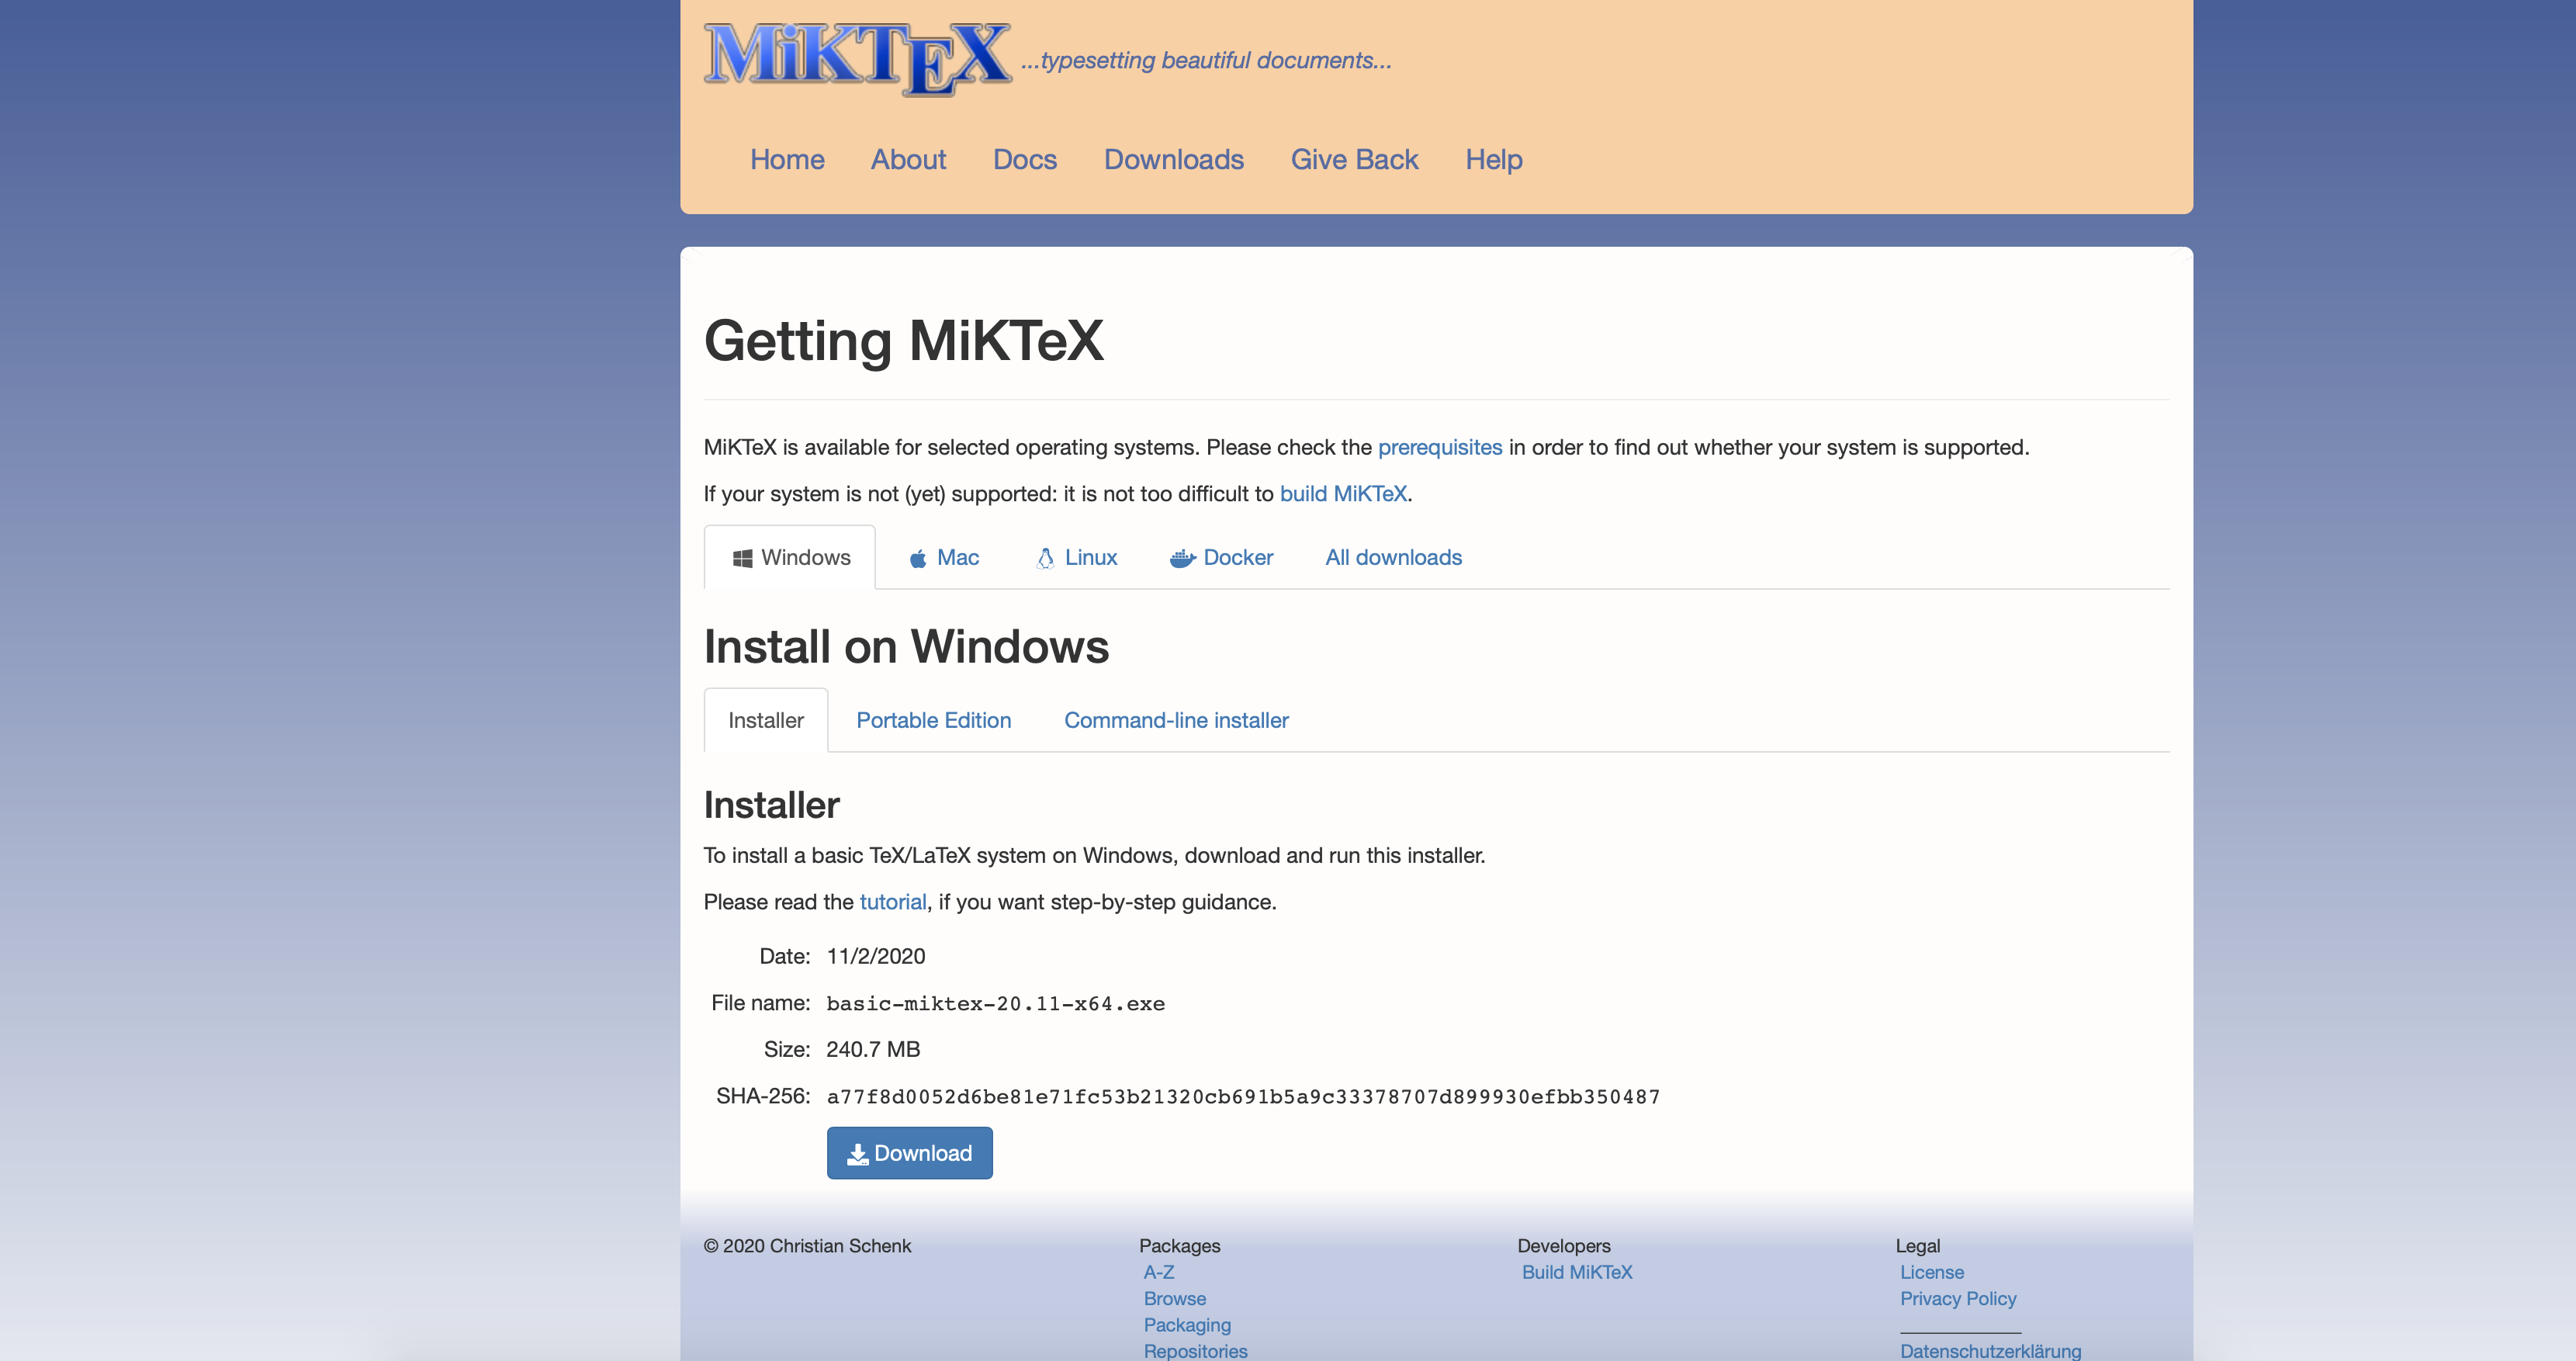
\includegraphics[width=1.0\textwidth]{./fig/miktex01}
  \caption{Site para download do MikTex.}
  \label{fig:miktex01}
  \fontefig{Elaborada pelo autor.}
\end{figure}
\item Rode o programa baixado;
\item Aceite os termos da \textit{copying conditions};
\begin{figure}[H]
  \centering
  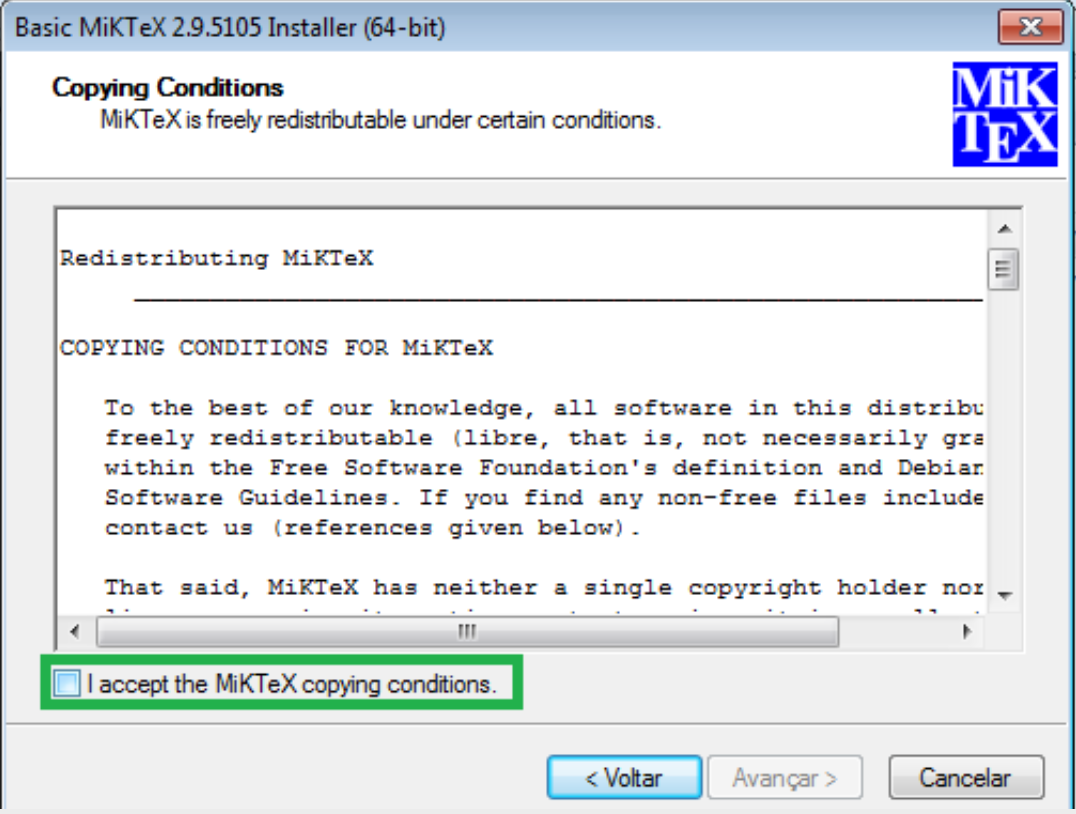
\includegraphics[width=0.6\textwidth]{./fig/miktex02}
  \caption{Instalação do MikTex - Aceitação dos termos.}
  \fontefig{Elaborada pelo autor.}
\end{figure}
\item Selecione instalar para todos os usuários do sistema;
\begin{figure}[H]
  \centering
  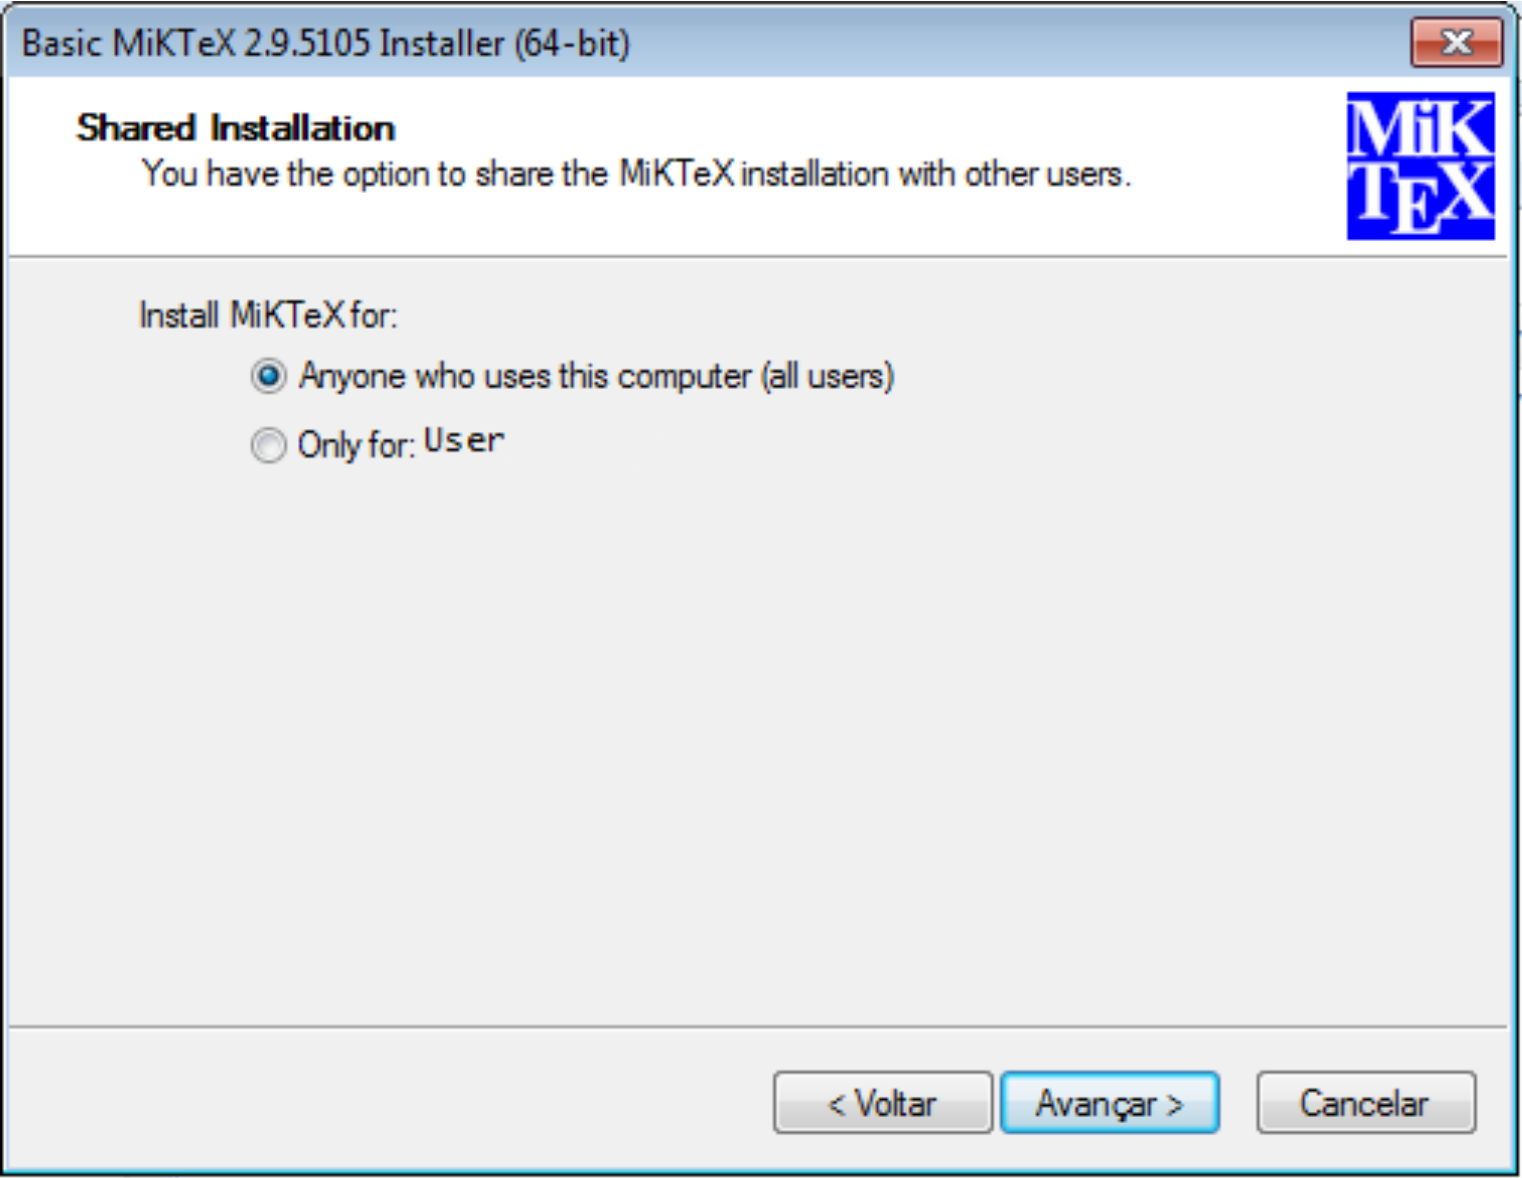
\includegraphics[width=0.6\textwidth]{./fig/miktex03}
  \caption{Instalação do MikTex - Seleção de usuários.}
  \fontefig{Elaborada pelo autor.}
\end{figure}
\item Escolha onde instalar o MiKTeX. É recomendado manter o local sugerido;
\begin{figure}[H]
  \centering
  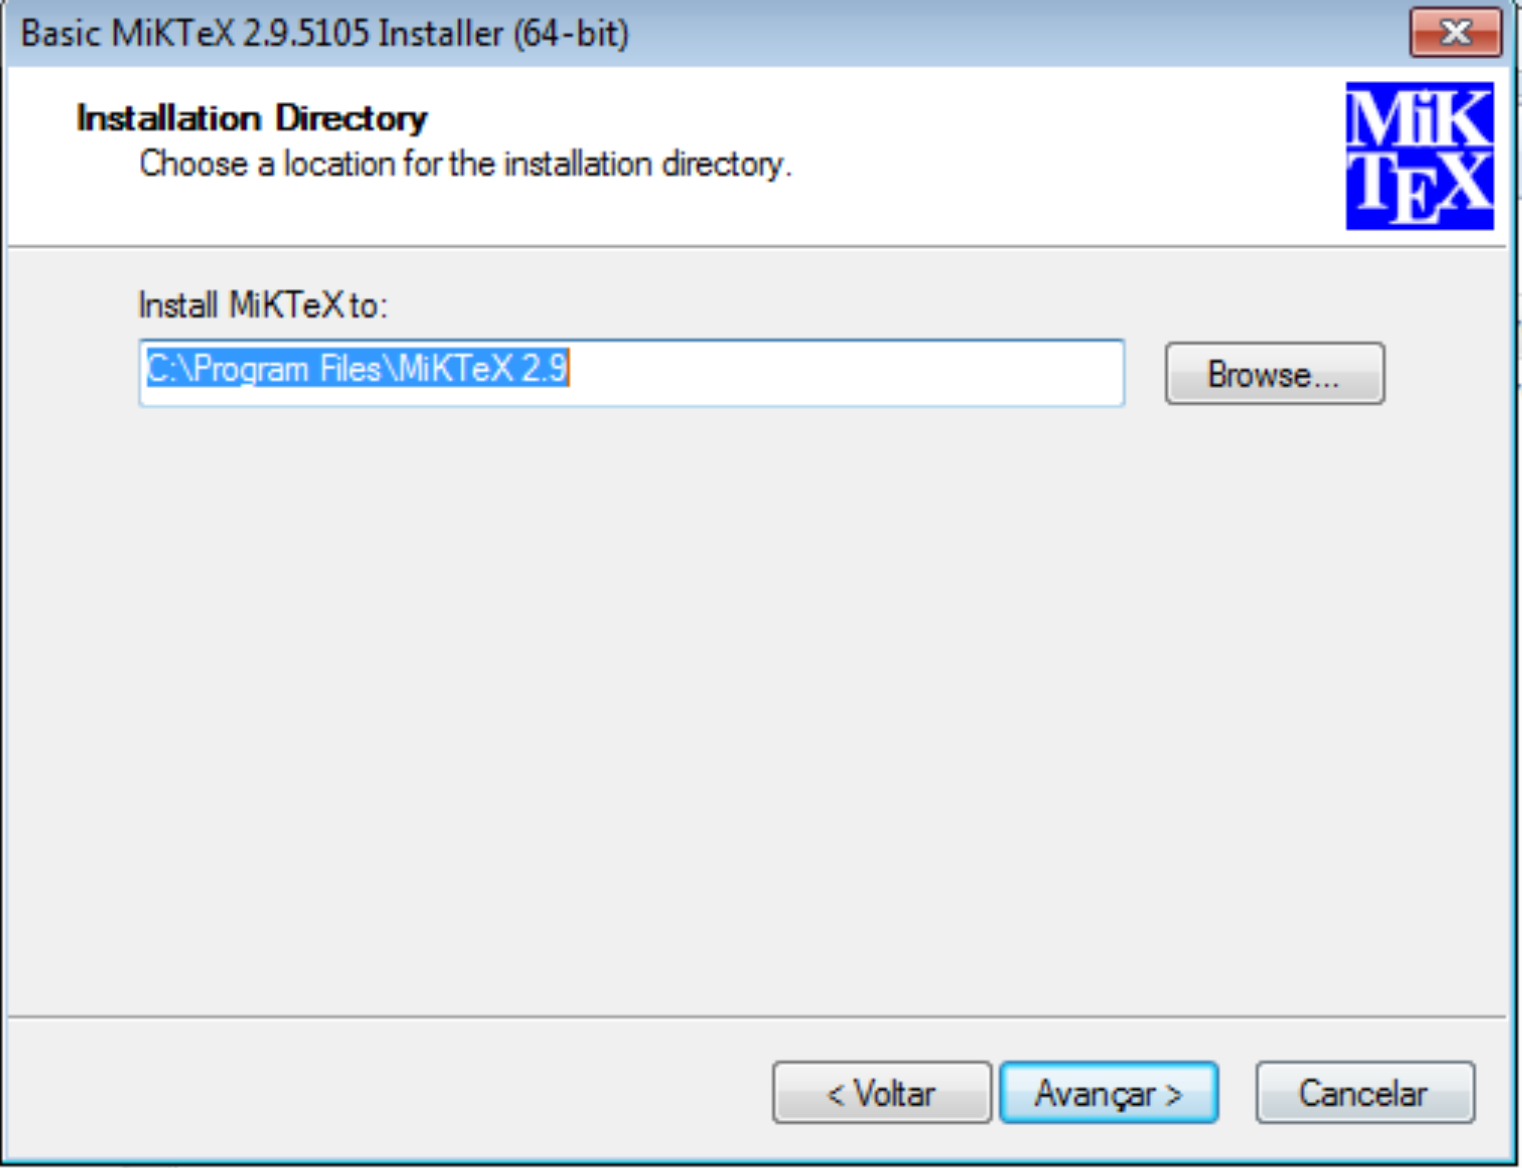
\includegraphics[width=0.6\textwidth]{./fig/miktex04}
  \caption{Instalação do MikTex - Local de instalação.}
  \fontefig{Elaborada pelo autor.}
\end{figure}
\item Escolha as opções solicitadas, é recomendado manter as sugestões A4 para o tipo de papel e \textbf{Ask me First} para instalar os pacotes faltantes;
\begin{figure}[H]
  \centering
  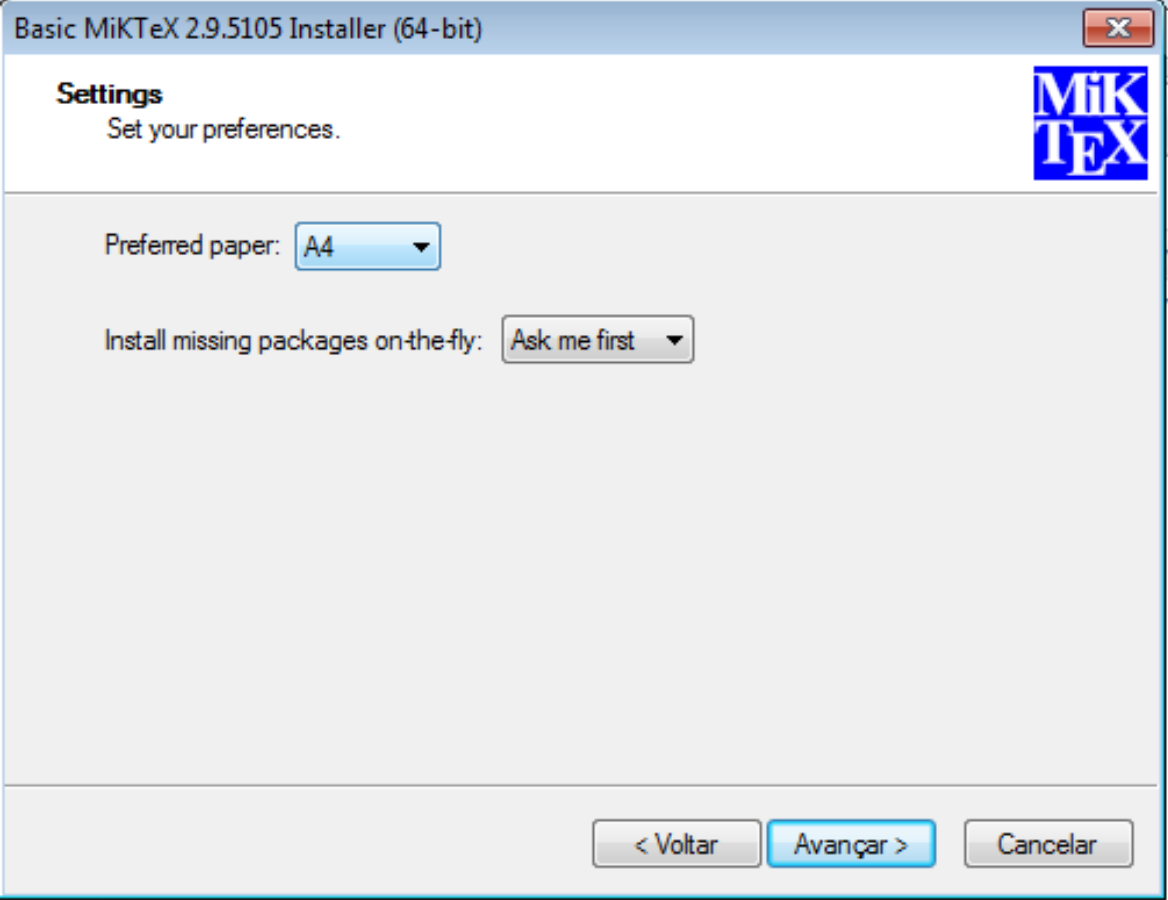
\includegraphics[width=0.6\textwidth]{./fig/miktex05}
  \caption{Instalação do MikTex - Seleção de opções.}
  \fontefig{Elaborada pelo autor.}
\end{figure}
\item Clique em \textbf{Start} para iniciar a instalação;
\begin{figure}[H]
  \centering
  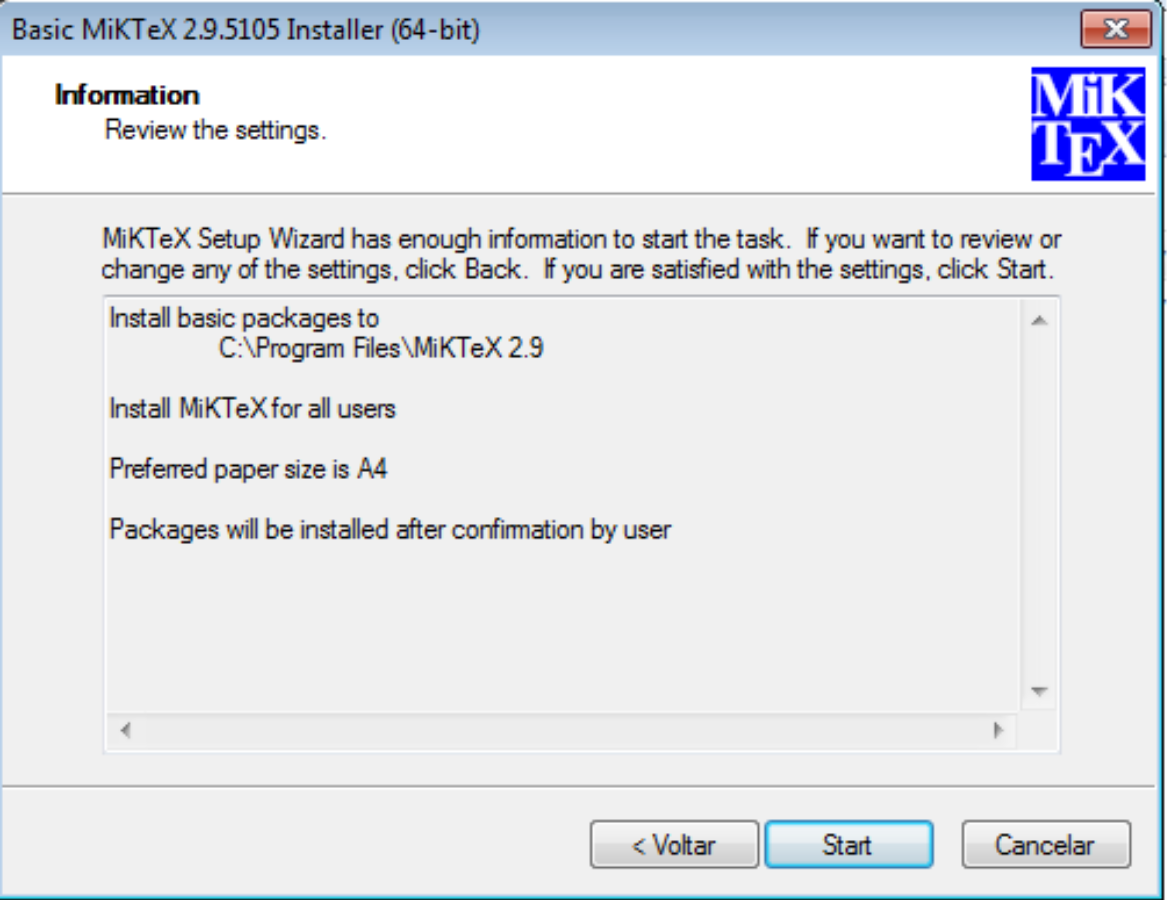
\includegraphics[width=0.6\textwidth]{./fig/miktex06}
  \caption{Instalação do MikTex - Início da instalação.}
  \fontefig{Elaborada pelo autor.}
\end{figure}
\item Autorize que o programa faça alterações no sistema;
\item Aguarde o final da instalação;
\begin{figure}[H]
  \centering
  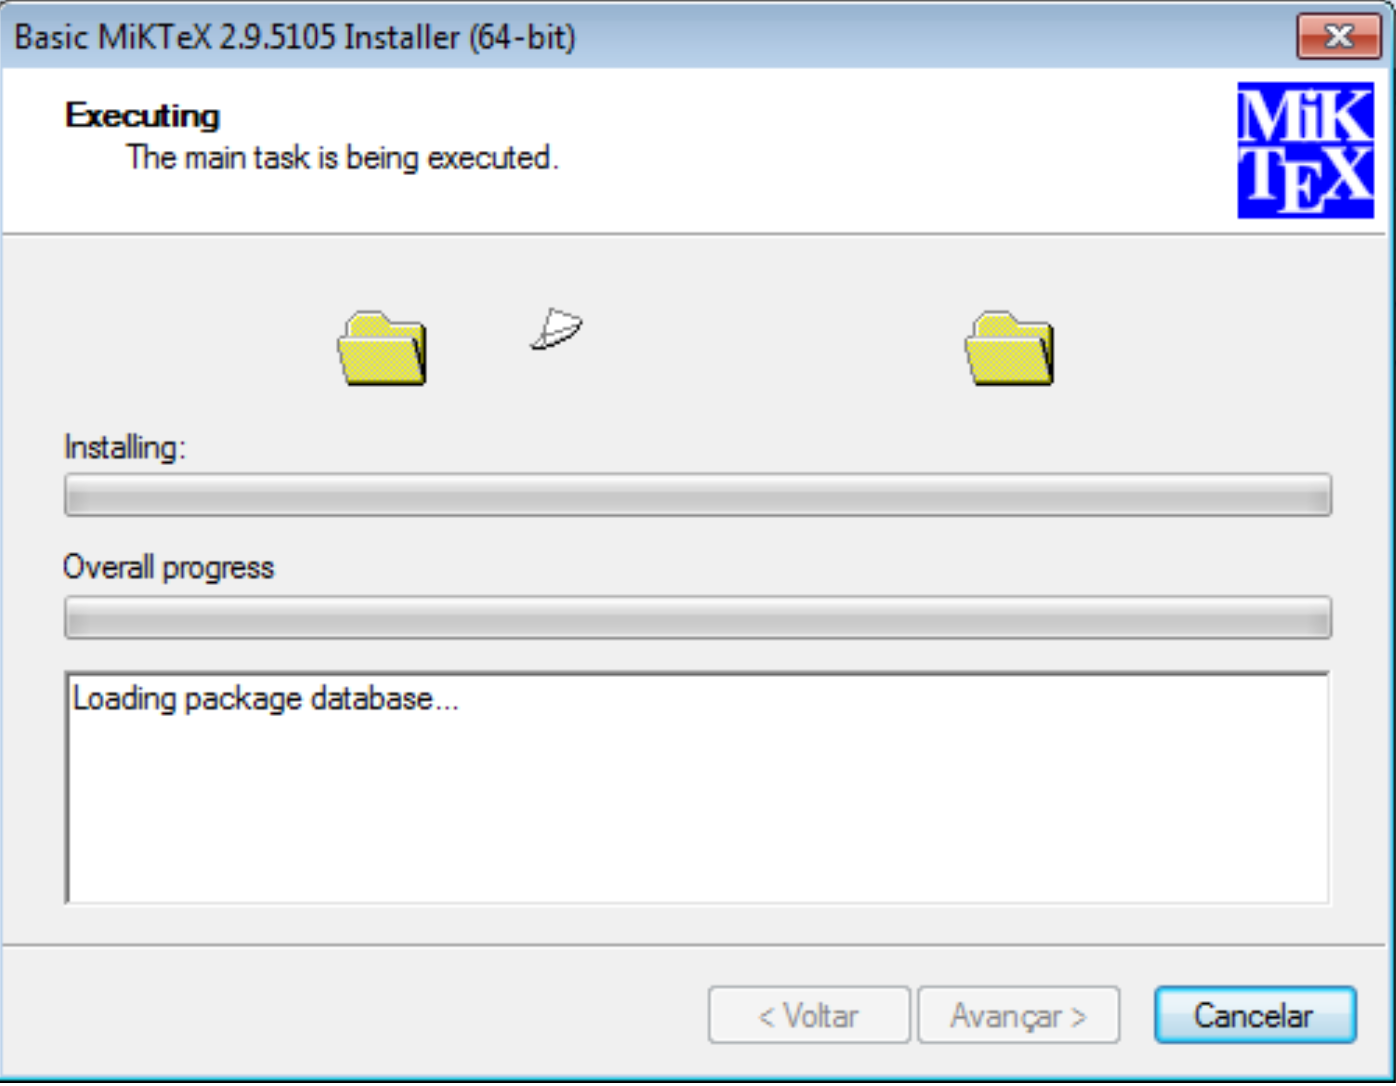
\includegraphics[width=0.6\textwidth]{./fig/miktex07}
  \caption{Instalação do MikTex - Execução da instalação.}
  \fontefig{Elaborada pelo autor.}
\end{figure}
\item Permita que o MikTeX busque por atualizações na internet;
\item Se desejar, desabilite a opção \textbf{Tell me more};
\item Conclua a instalação clicando em \textbf{Close}.
\begin{figure}[H]
  \centering
  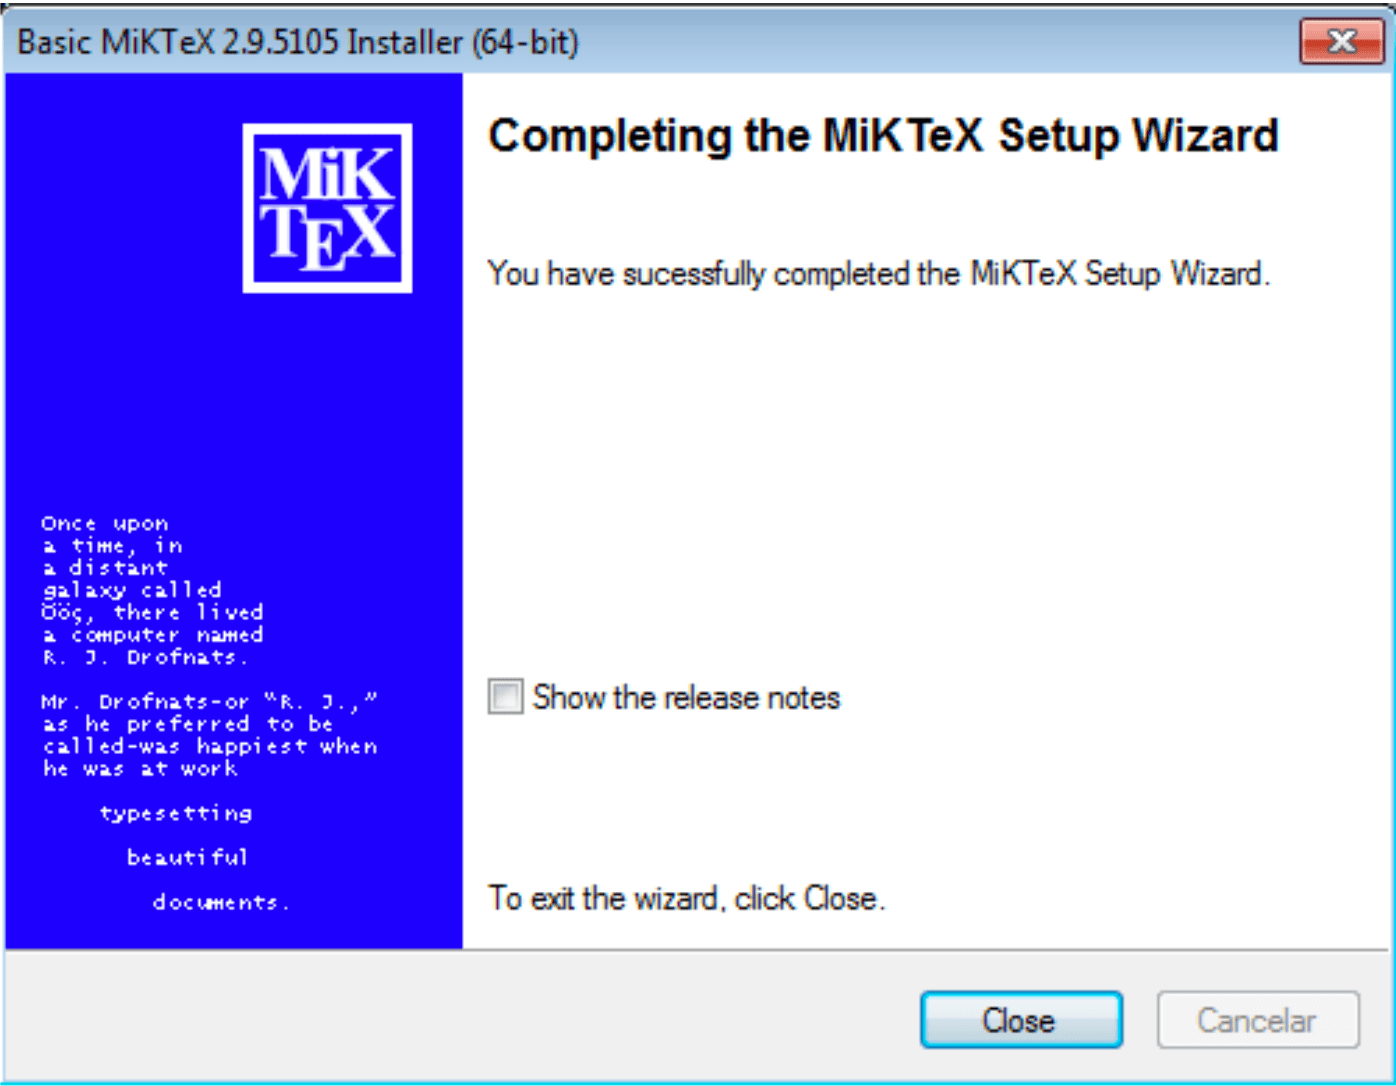
\includegraphics[width=0.6\textwidth]{./fig/miktex08}
  \caption{Instalação do MikTex - Fim da instalação.}
  \fontefig{Elaborada pelo autor.}
\end{figure}
\end{enumerate}

\subsection{Instalação Completa do MikTeX}

\textbf{ATENÇÃO:} A versão completa do MiKTeX é chamada Net \textbf{Installer} e não está na página inicial de download da página do MikTeX.

O processo de instalação da versão básica é simples, sendo exatamente igual ao processo de instalação de qualquer outro programa. Já a versão completa, é necessário abrir o instalador duas vezes. A primeira tem o objetivo de baixar e escolher uma pasta para armazenar os arquivos necessários. Uma vez baixado todos os arquivos, é necessário abrir o instalador novamente e indicar a pasta onde os arquivos foram baixados. Em seguida, o MikTeX será instalado.
 
O passo a passo para a instalação do MikTeX completo pode ser visto a seguir \cite{miktexfull}.

\begin{enumerate}
\item Entre na página de downloads do MiKTeX: \url{http://miktex.org/download} (\autoref{fig:miktex01});
\item \textbf{NÃO} clique no botão de download;
\item Selecione a aba \textbf{All Downloads};
\begin{figure}[H]
  \centering
  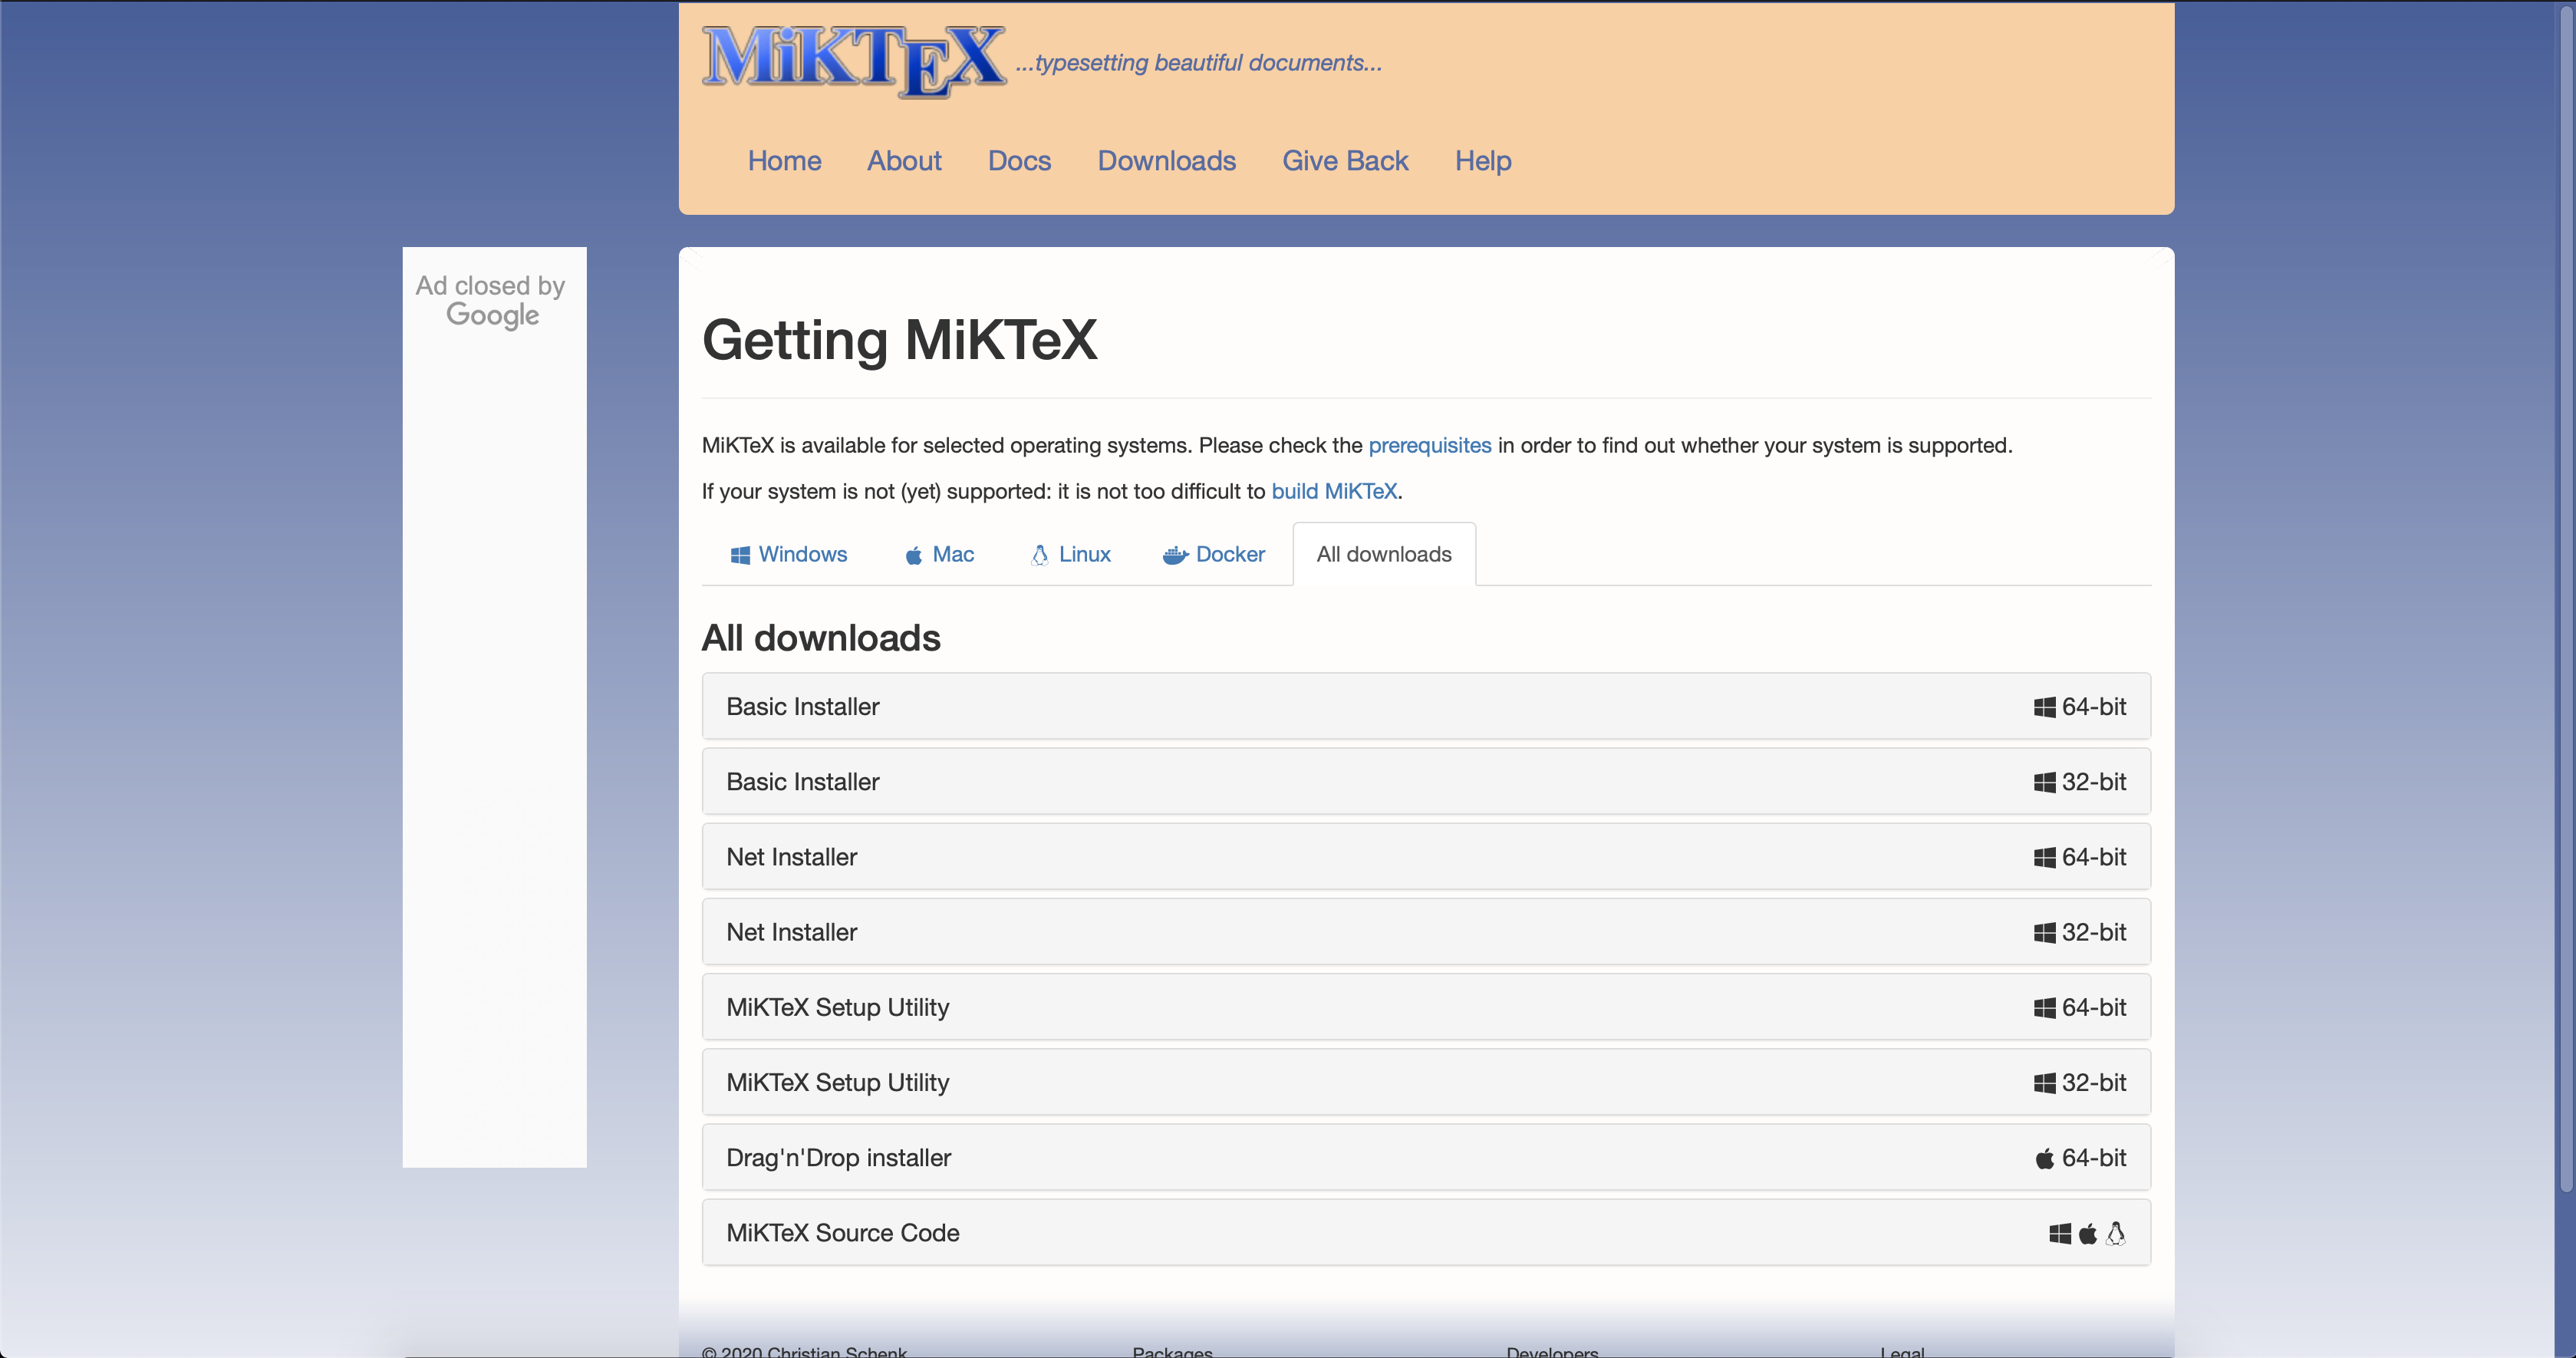
\includegraphics[width=1.0\textwidth]{./fig/miktex09}
  \caption{Instalação completa do MikTex - Página com todos os downloads.}
  \fontefig{Elaborada pelo autor}
\end{figure}
\item Selecione a opção \textbf{Net Installer}, escolha 32 ou 64 bits de acordo com seu computador;
\begin{figure}[H]
  \centering
  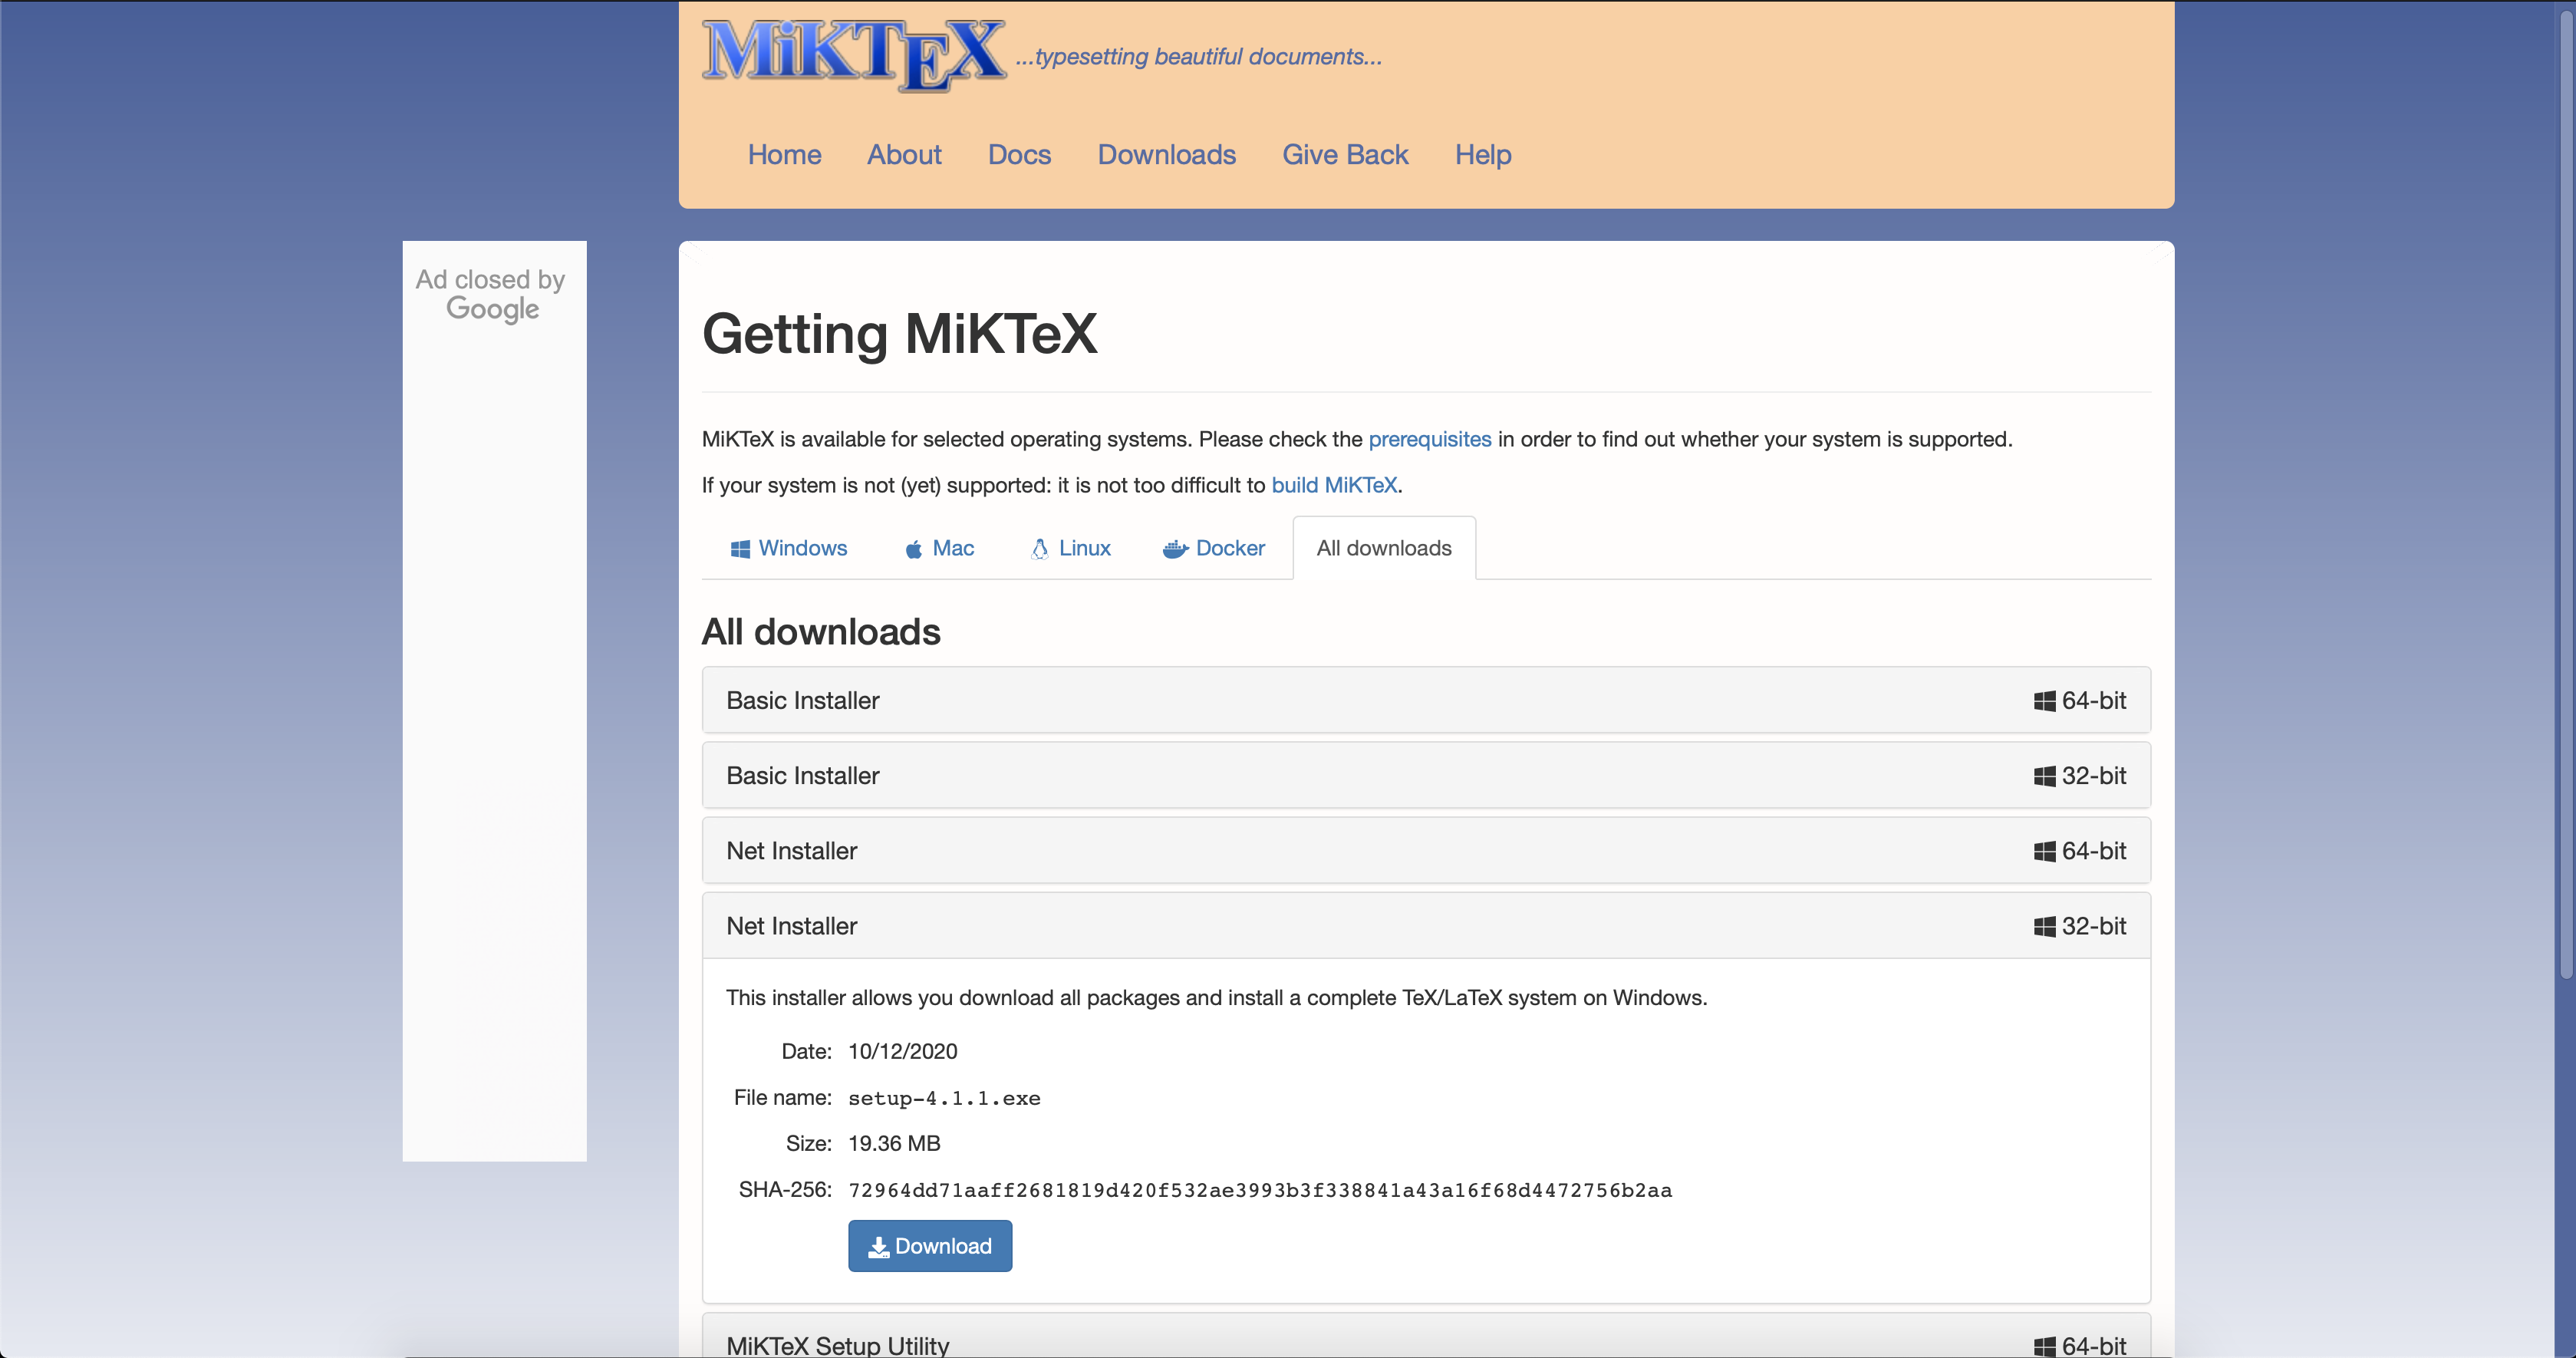
\includegraphics[width=1.0\textwidth]{./fig/miktex10}
  \caption{Instalação  completa do MikTex - Página com net installer.}
  \fontefig{Elaborada pelo autor}
\end{figure}
\item Clique em download para baixar o arquivo de instalação;
\item Abra o instalador e aceite as condições de uso para continuar;
\begin{figure}[H]
  \centering
  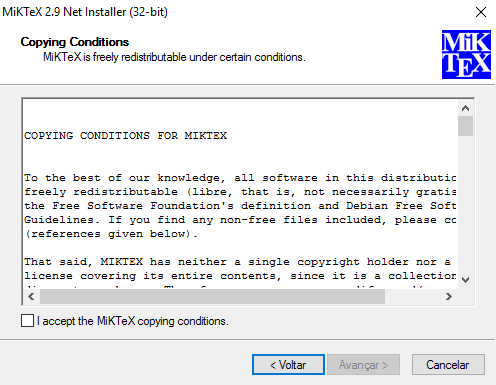
\includegraphics[width=0.6\textwidth]{./fig/miktex11}
  \caption{Instalação completa do MikTex - Primeira página do instalador MikTeX.}
  \fontefig{\cite{miktexfull}}
\end{figure}
\item Baixar o MikTeX;
Agora é possível escolher baixar ou instalar o MikTeX. Escolha a opção de baixar e clique em avançar.
\begin{figure}[H]
  \centering
  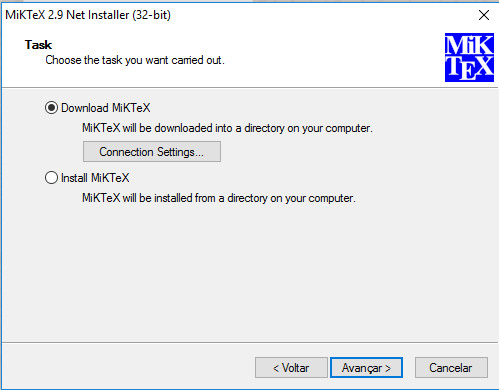
\includegraphics[width=0.6\textwidth]{./fig/miktex12}
  \caption{Instalação completa do MikTex - Segunda tela do instalador do MikTeX.}
  \fontefig{\cite{miktexfull}}
\end{figure}
\item Escolha o tipo de download que deve ser feito.
Escolha qual versão do MikTeX você deseja instalar. O ideal é a instalação completa, que ocupa mais espaço em disco. Se preferir, pode escolher a versão básica para economizar espaço em disco e baixar pacotes adicionais conforme for precisando deles (como na seção anterior). Após escolher uma opção, clique em Avançar.
\begin{figure}[H]
  \centering
  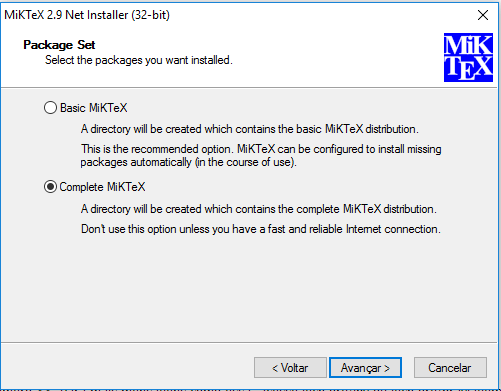
\includegraphics[width=0.6\textwidth]{./fig/miktex13}
  \caption{Instalação completa do MikTex - Tipo de distribuição: básica ou completa.}
  \fontefig{\cite{miktexfull}}
\end{figure}
\item Escolha de onde você deseja baixar.
Nesse passo, é necessário escolher de qual servidor você deseja baixar o MikTeX. É recomendado que você escolha o servidor que estiver mais próximo de onde você estiver acessando a internet. Uma vez escolhido o servidor, o botão Avançar será habilitado e você poderá prosseguir com a instalação.
\begin{figure}[H]
  \centering
  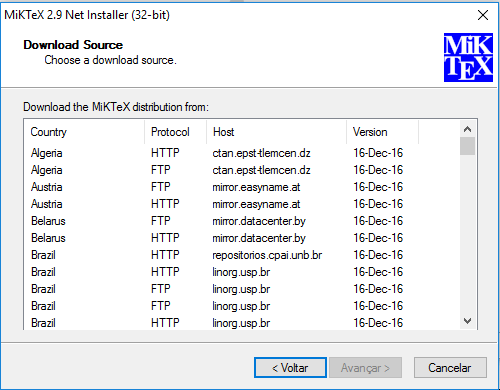
\includegraphics[width=0.6\textwidth]{./fig/miktex14}
  \caption{Instalação completa do MikTex - Lista de servidores que permitem o download do MikTeX.}
  \fontefig{\cite{miktexfull}}
\end{figure}
\item Escolha o local do seu computador onde os arquivos devem ser salvos.
Agora é necessário que você determine uma pasta do seu computador para que os arquivos sejam baixados. É importante que seja um local fácil, já que posteriormente será necessário indicar para o instalador do MikTeX essa mesma pasta para que a instalação seja iniciada. Uma vez escolhida uma pasta, basta continuar.
\begin{figure}[H]
  \centering
  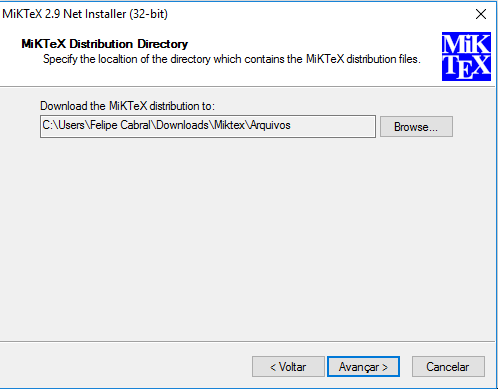
\includegraphics[width=0.6\textwidth]{./fig/miktex15}
  \caption{Instalação completa do MikTex - Determine o local onde os arquivos devem ser salvos em seu computador.}
  \fontefig{\cite{miktexfull}}
\end{figure}
\item Revise suas opções e inicie o download.
Se estiver tudo certo, clique em \textbf{Start} e o download será iniciado. Assim que terminar o download, você poderá finalizar o instalador.
\begin{figure}[H]
  \centering
  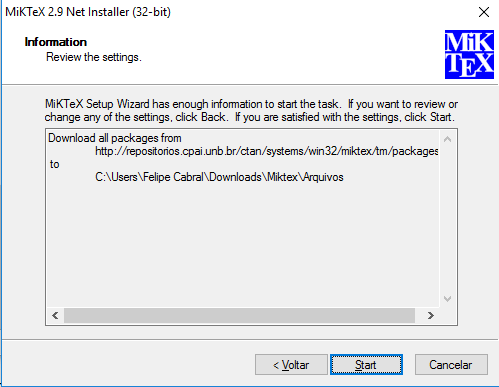
\includegraphics[width=0.6\textwidth]{./fig/miktex16}
  \caption{Instalação completa do MikTex - Resumo das opções escolhidas para iniciar o download.}
  \fontefig{\cite{miktexfull}}
\end{figure}
\item Instalação do MikTeX.
Uma vez terminado o download, é necessário dar início ao processo de instalação do MikTeX. Para isso, abra novamente o instalador e escolha a opção \textbf{Install MikTeX} para que o processo de instalação se inicie.
\begin{figure}[H]
  \centering
  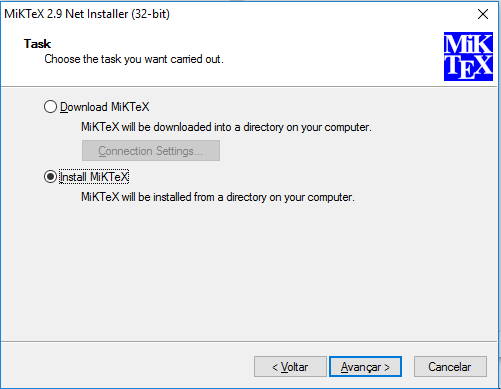
\includegraphics[width=0.6\textwidth]{./fig/miktex17}
  \caption{Instalação completa do MikTex - Instalação do MikTeX após o download concluído.}
  \fontefig{\cite{miktexfull}}
\end{figure}
\item Escolha o tipo de distribuição.
\begin{figure}[H]
  \centering
  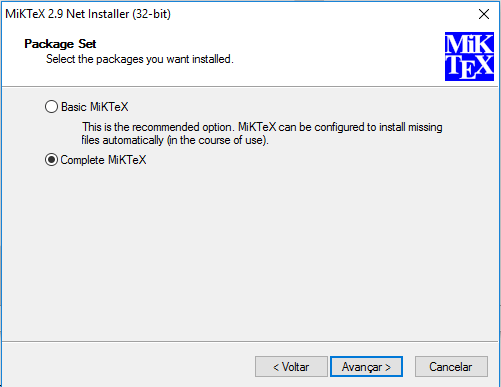
\includegraphics[width=0.6\textwidth]{./fig/miktex18}
  \caption{Instalação completa do MikTex - Escolha entre a versão básica e a completa. Basta escolher a que você baixou.}
  \fontefig{\cite{miktexfull}}
\end{figure}
\item Escolha a pasta onde o download do MikTeX foi realizado.
Nesse momento, é necessário escolher a pasta onde o download do MikTeX foi realizado. Geralmente, o instalador preenche o caminho para a pasta escolhida automaticamente, mas você pode alterar a pasta clicando em \textbf{Browse} caso o caminho esteja errado.
\begin{figure}[H]
  \centering
  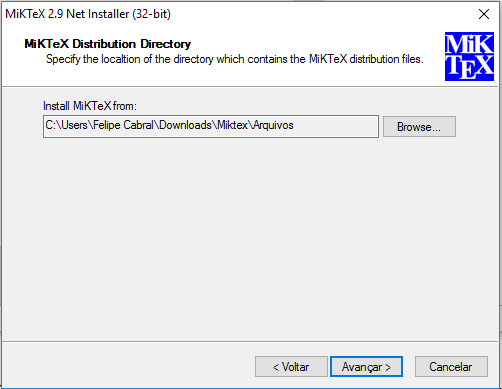
\includegraphics[width=0.6\textwidth]{./fig/miktex19}
  \caption{Instalação completa do MikTex - Escolha a pasta onde o MikTeX foi baixado.}
  \fontefig{\cite{miktexfull}}
\end{figure}
\item Escolha o local de instalação.
Finalmente, escolha o local onde o MikTeX deve ser instalado em seu computador e prossiga com a instalação. 
\begin{figure}[H]
  \centering
  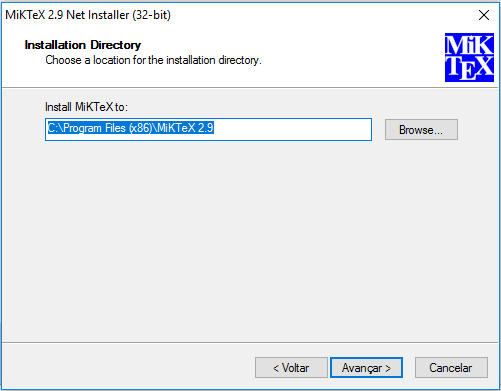
\includegraphics[width=0.6\textwidth]{./fig/miktex20}
  \caption{Instalação completa do MikTex - Local onde o MikTeX será instalado em seu computador.}
  \fontefig{\cite{miktexfull}}
\end{figure}
\end{enumerate}

\section{Instalando o editor}

Para realizar a edição de documentos \LaTeX\ no computador, além do compilador MikTex é necessário instalar o editor. Neste documento, para o sistema operacional Windows é sugerido o uso do TeXnicCenter, cuja instalação é detalhada a seguir \cite{texnic}.

\begin{enumerate}
\item Faça o download do arquivo de instalação disponível em \url{https://www.texniccenter.org/download/}. Selecione a opção de acordo com a versão do seu sistema operacional. 
\item Abra o arquivo baixado.
\item Se uma janela de aviso de segurança for aberta apenas clique na opção \aspas{Executar} para prosseguir a instalação, caso contrário vá para o passo seguinte.
\begin{figure}[H]
  \centering
  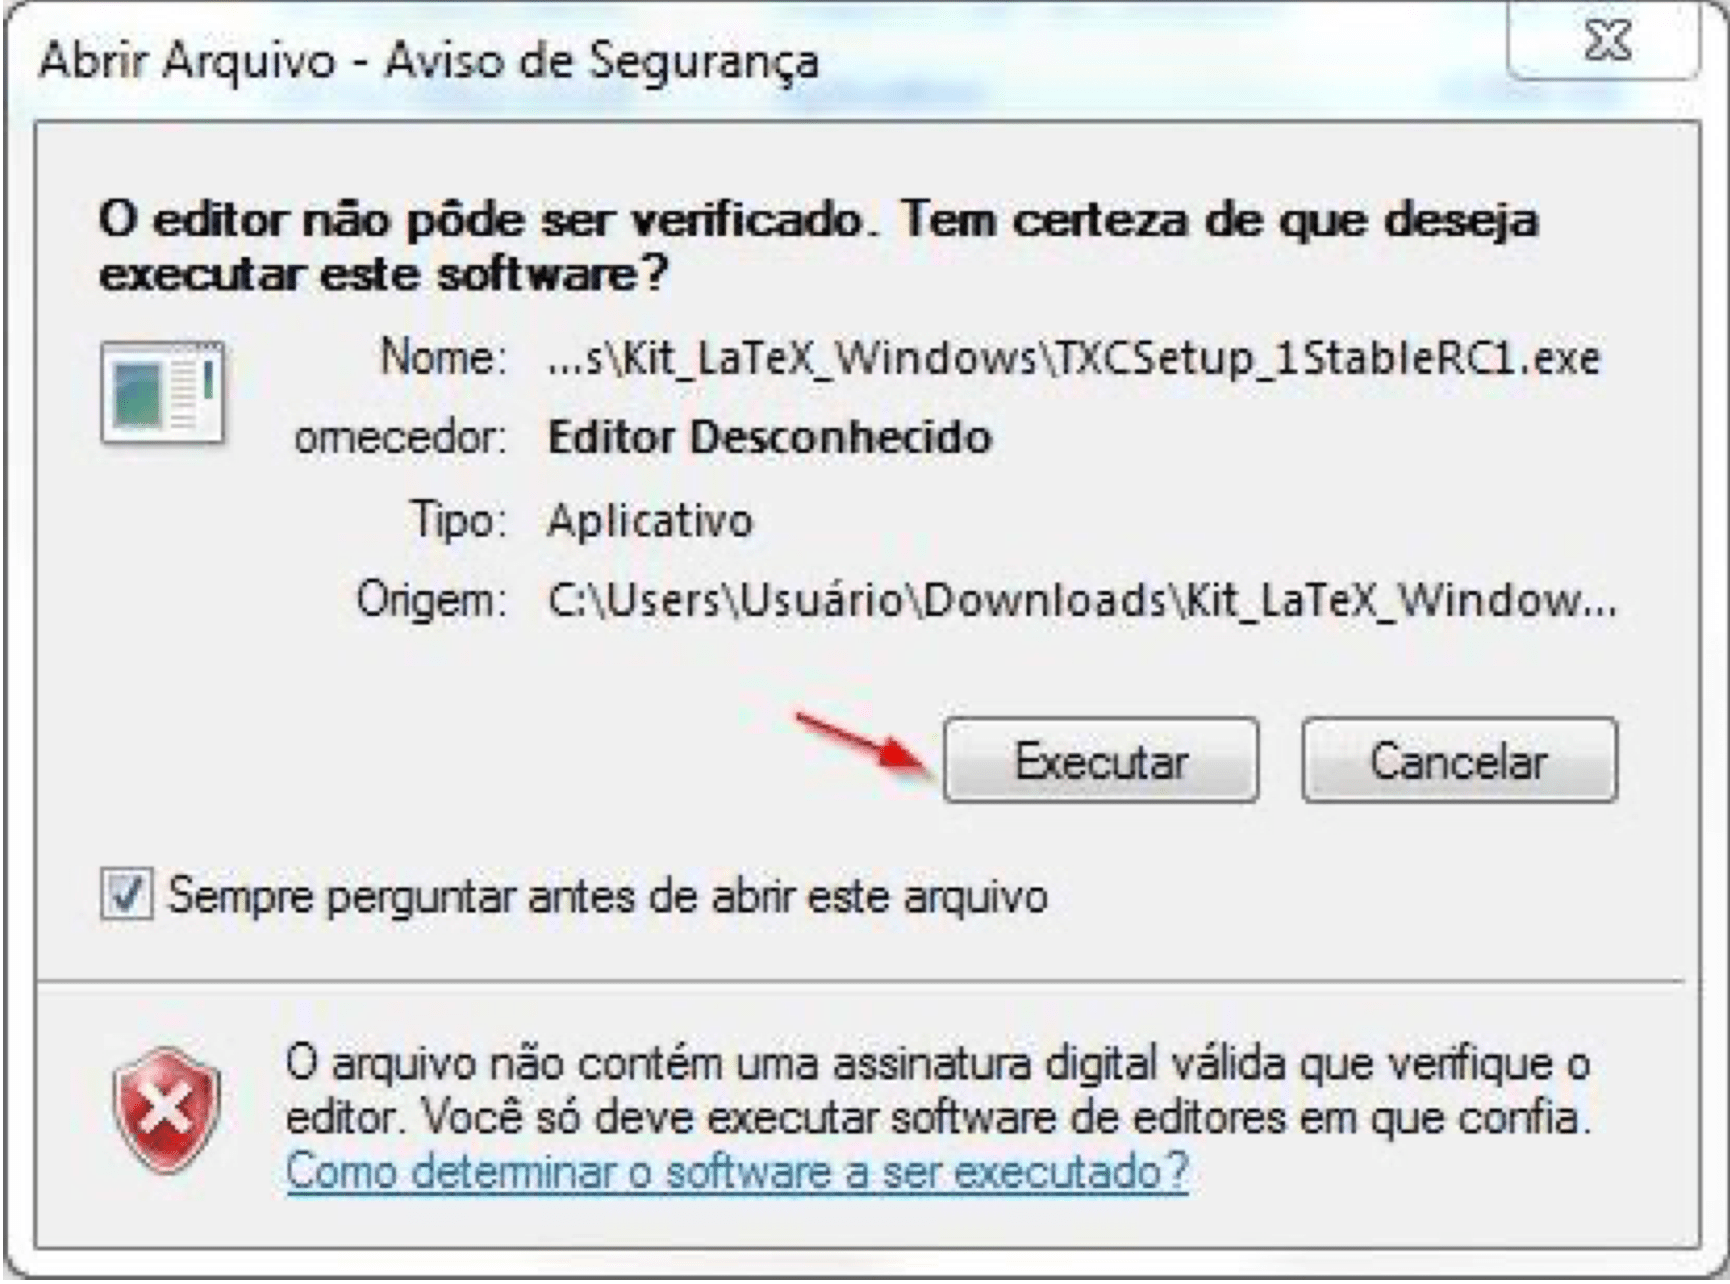
\includegraphics[width=0.6\textwidth]{./fig/texniccenter01}
  \caption{Instalação do TeXnicCenter - Aviso de segurança.}
  \fontefig{\cite{texnic}}
\end{figure}
\item Para iniciar o processo de instalação na tela exibida clique no botão \textbf{Next}.
\begin{figure}[H]
  \centering
  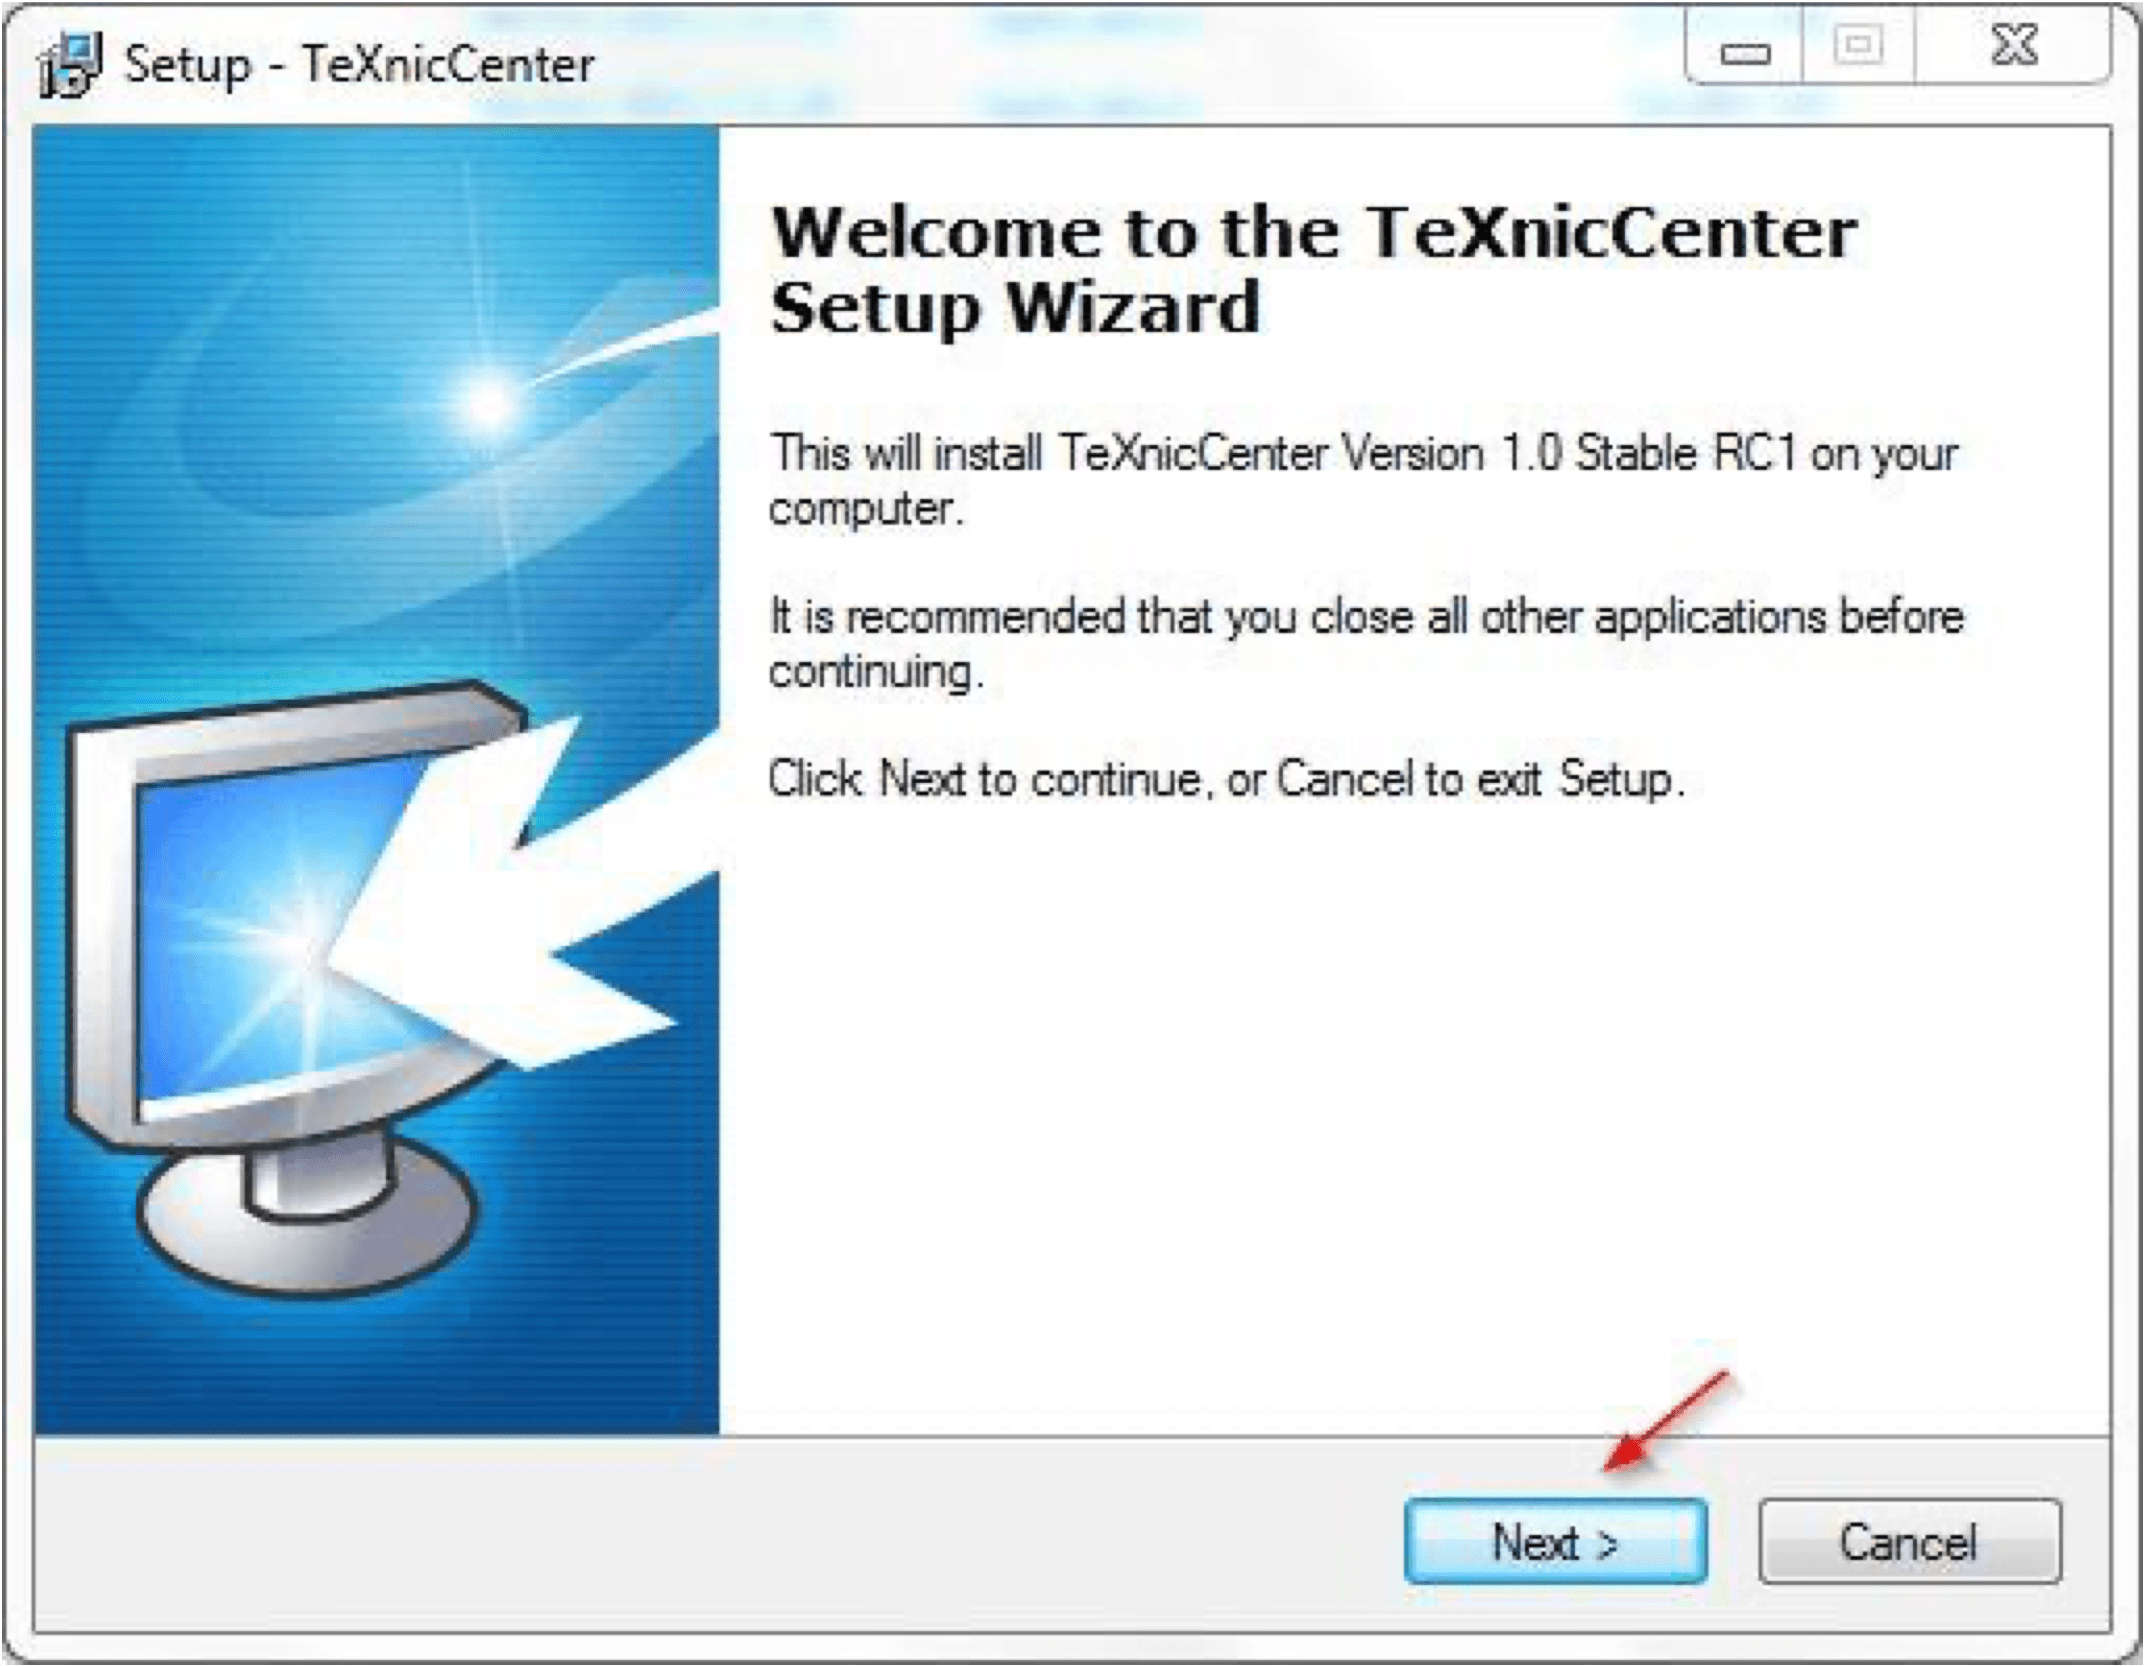
\includegraphics[width=0.6\textwidth]{./fig/texniccenter02}
  \caption{Instalação do TeXnicCenter - Primeira tela.}
  \fontefig{\cite{texnic}}
\end{figure}
\item É necessário aceitar a licença de uso do software selecionando a opção \textbf{I accept the agreement}.
\begin{figure}[H]
  \centering
  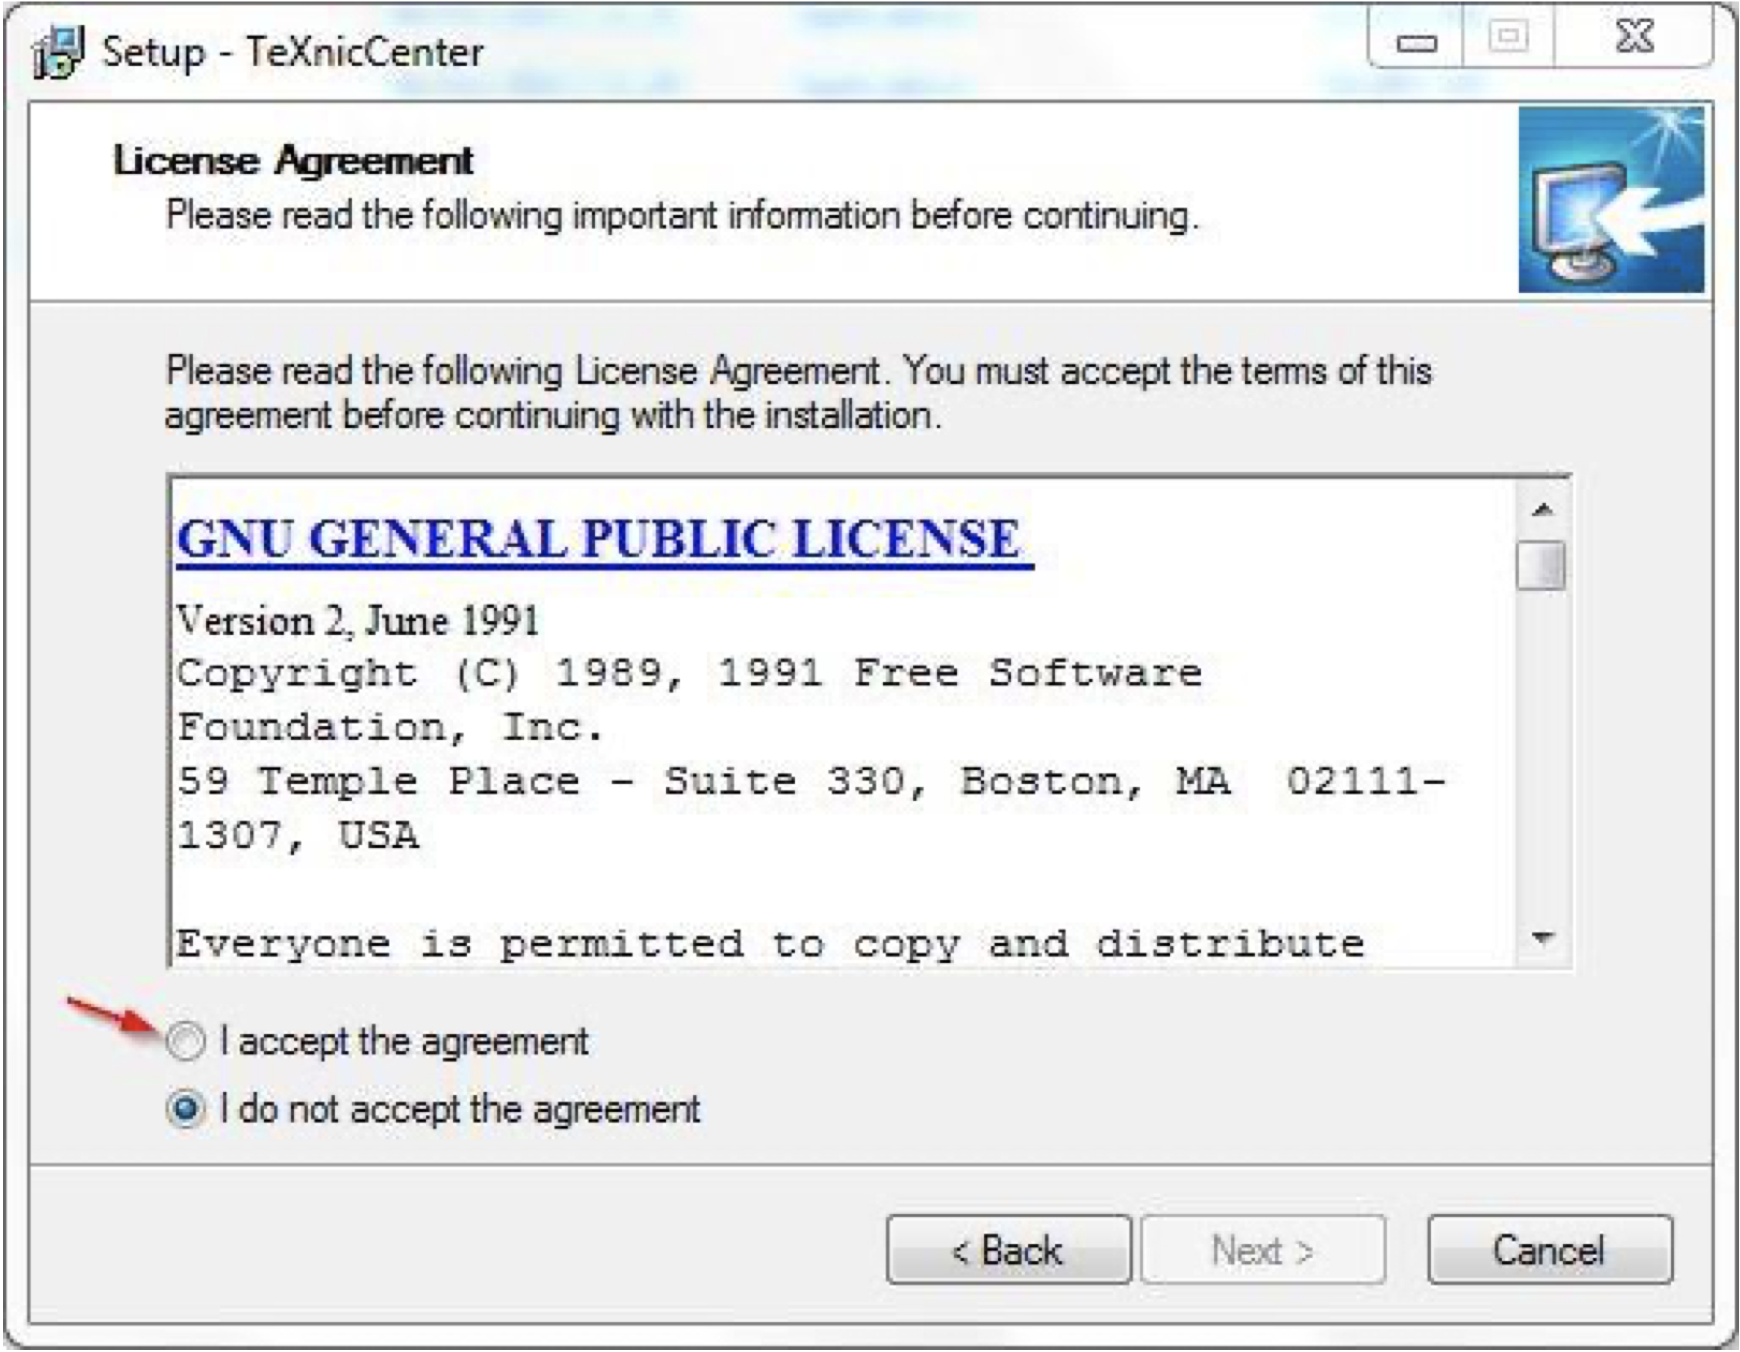
\includegraphics[width=0.6\textwidth]{./fig/texniccenter03}
  \caption{Instalação do TeXnicCenter - Segunda tela.}
  \fontefig{\cite{texnic}}
\end{figure}
\item Após aceitar a licença do software clique no botão \textbf{Next}.
\begin{figure}[H]
  \centering
  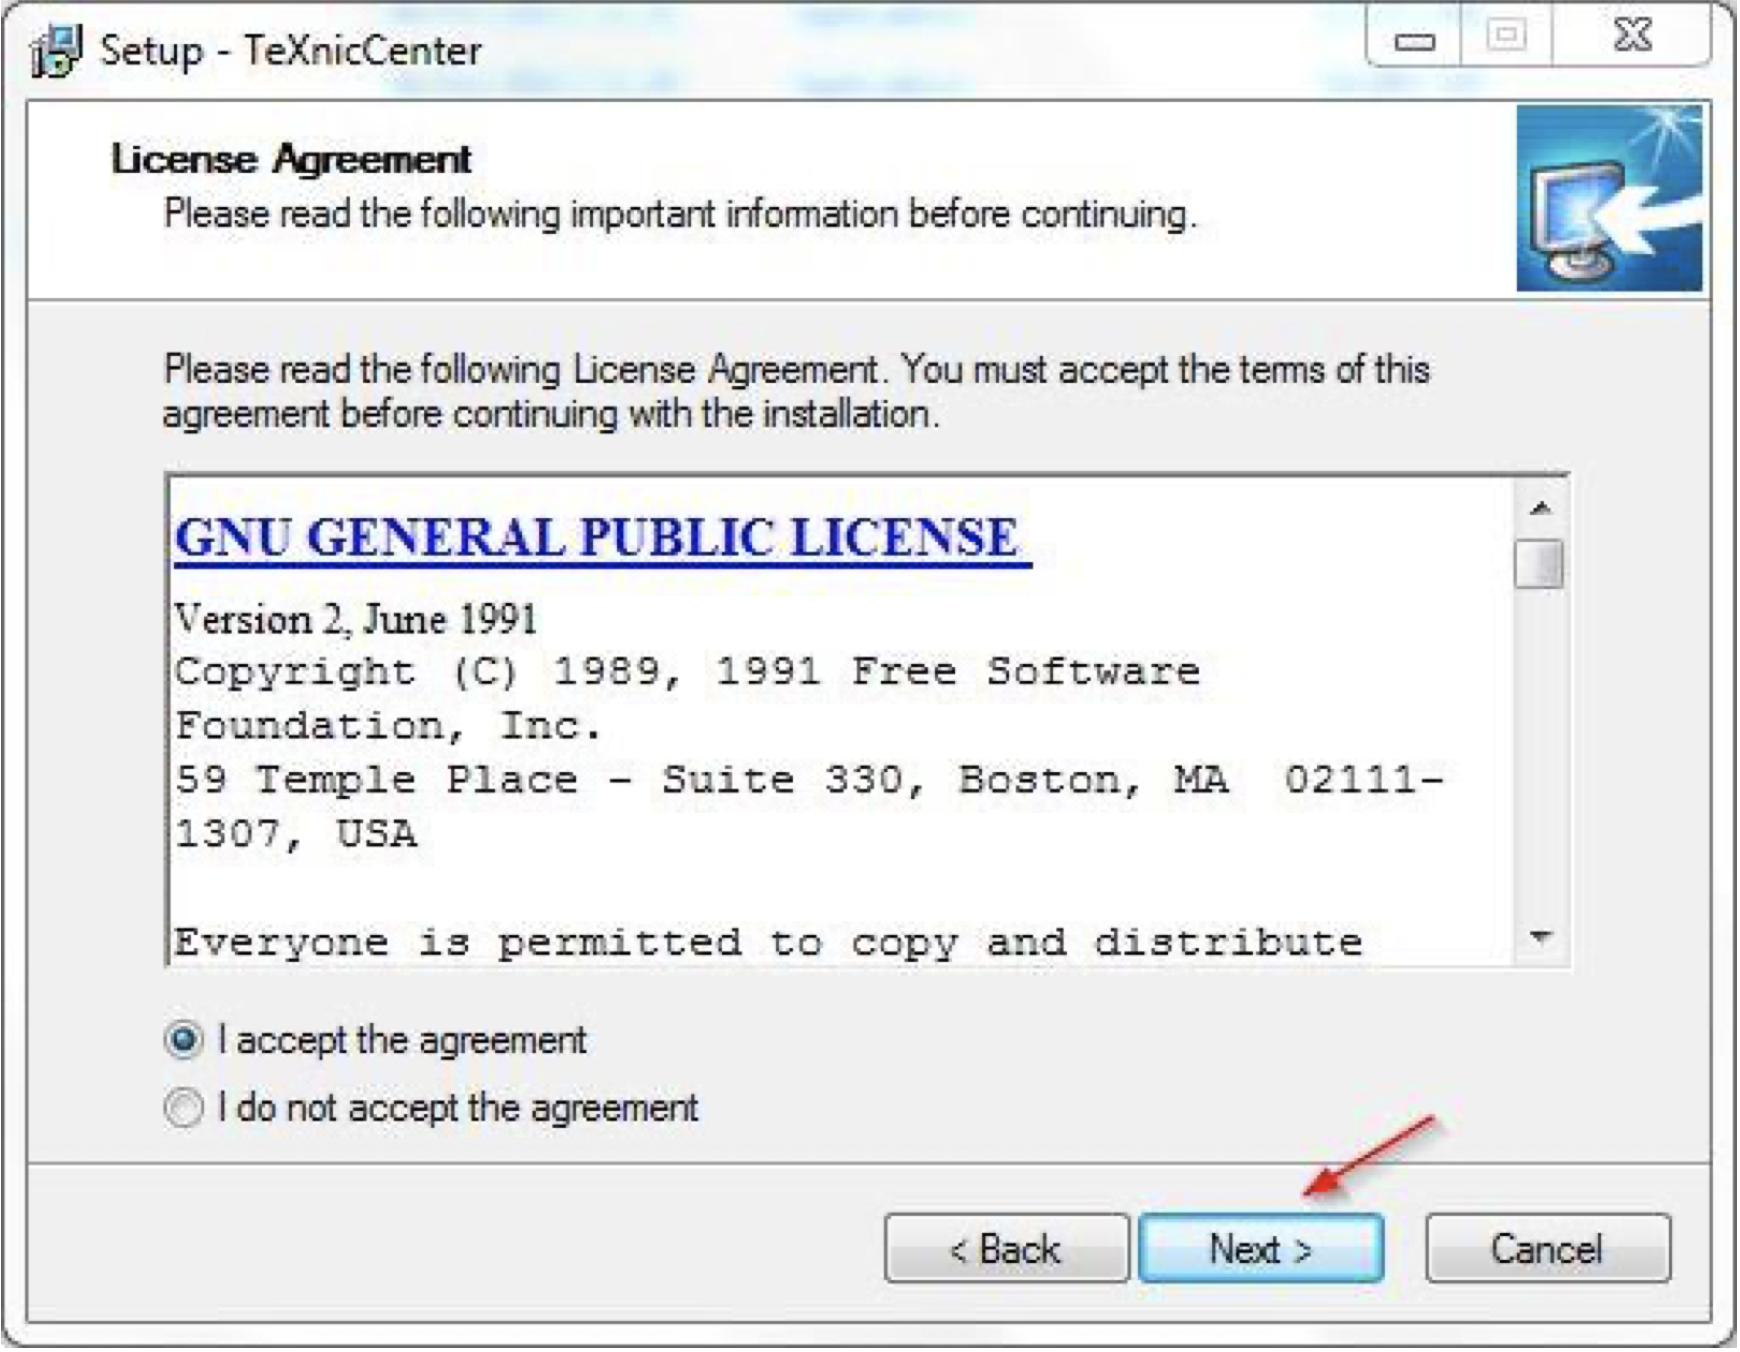
\includegraphics[width=0.6\textwidth]{./fig/texniccenter04}
  \caption{Instalação do TeXnicCenter - Segunda tela (após aceitar termos).}
  \fontefig{\cite{texnic}}
\end{figure}
\item Agora é apresentado o local onde o software será instalado, não é necessário selecionar outra pasta, copie o local indicado como padrão (neste tutorial é o: \aspas{C:$\backslash$Program Files (x86)$\backslash$TeXnicCenter}, mas pode variar dependendo da versão do Windows utilizado) para posteriormente instalar o corretor ortográfico Vero. Clique em \textbf{Next} para continuar o processo de instalação.
\begin{figure}[H]
  \centering
  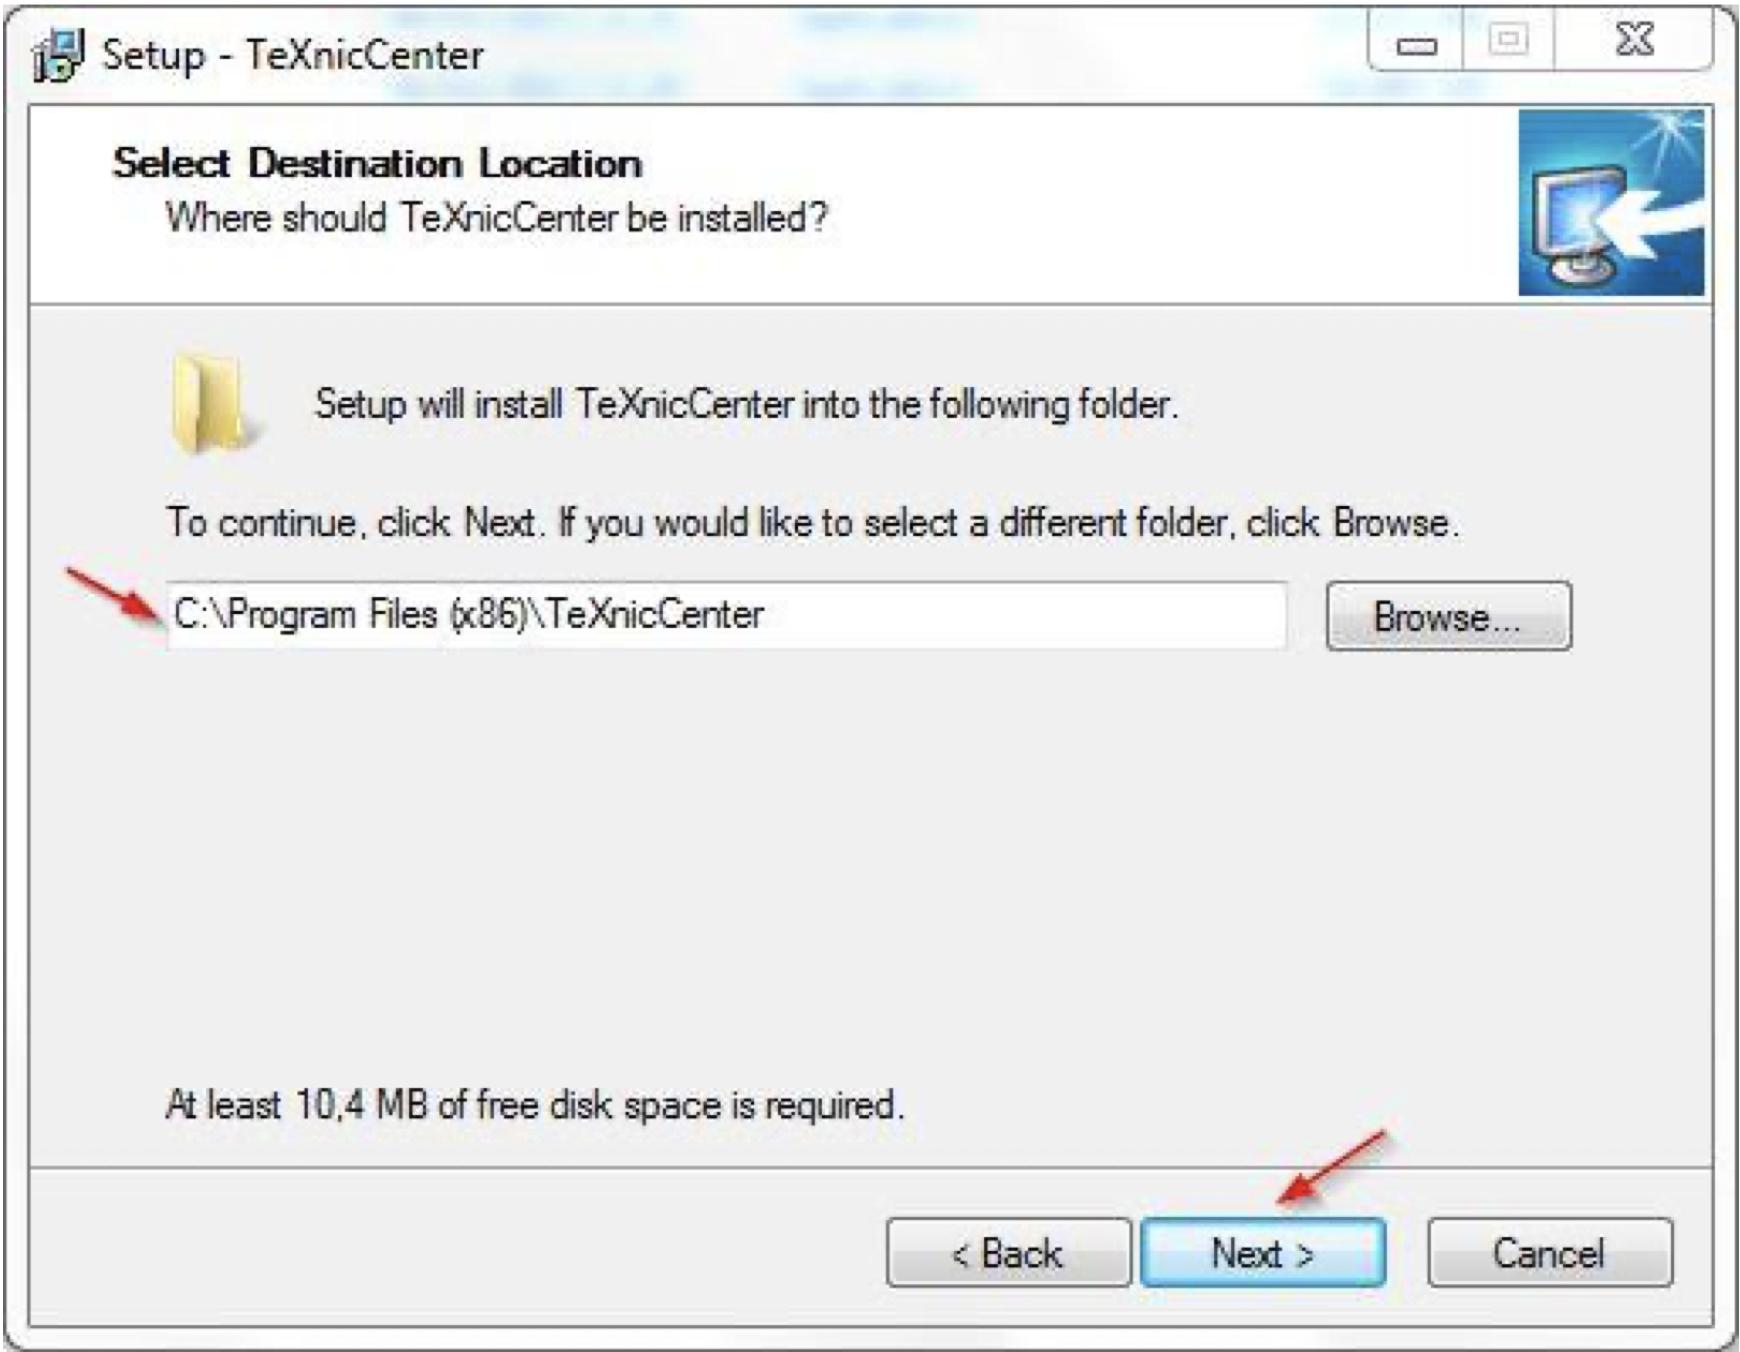
\includegraphics[width=0.6\textwidth]{./fig/texniccenter05}
  \caption{Instalação do TeXnicCenter - Terceira tela.}
  \fontefig{\cite{texnic}}
\end{figure}
\item A tela de seleção de componentes será exibida, não será necessário selecionar nenhuma opção apenas mantenha as opções selecionadas por padrão e clique no botão \textbf{Next} para continuar o processo.
\begin{figure}[H]
  \centering
  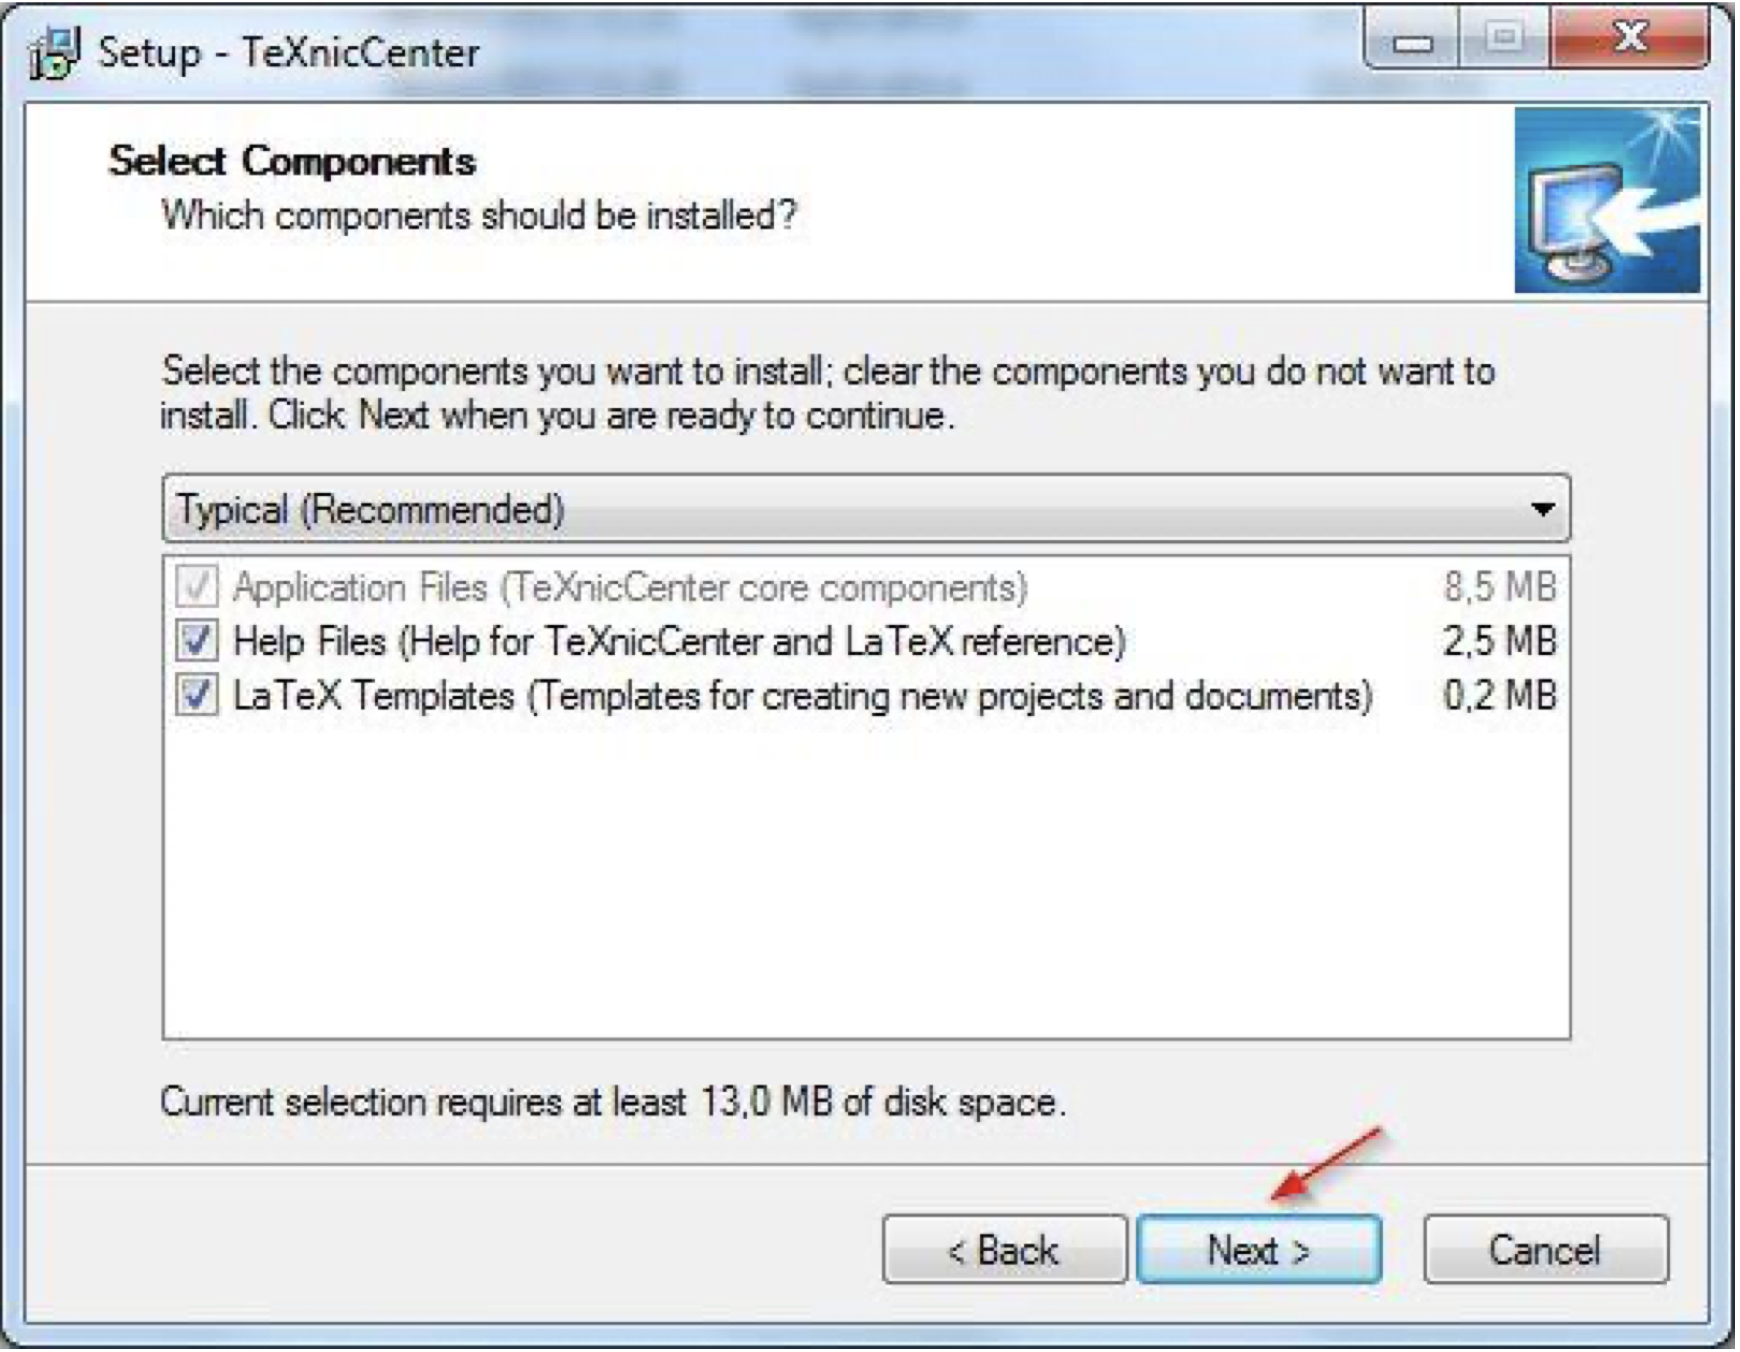
\includegraphics[width=0.6\textwidth]{./fig/texniccenter06}
  \caption{Instalação do TeXnicCenter - Quarta tela.}
  \fontefig{\cite{texnic}}
\end{figure}
\item Agora será exibida a opção para a criação os ícones do software no menu do Windows, apenas clique em \textbf{Next}.
\begin{figure}[H]
  \centering
  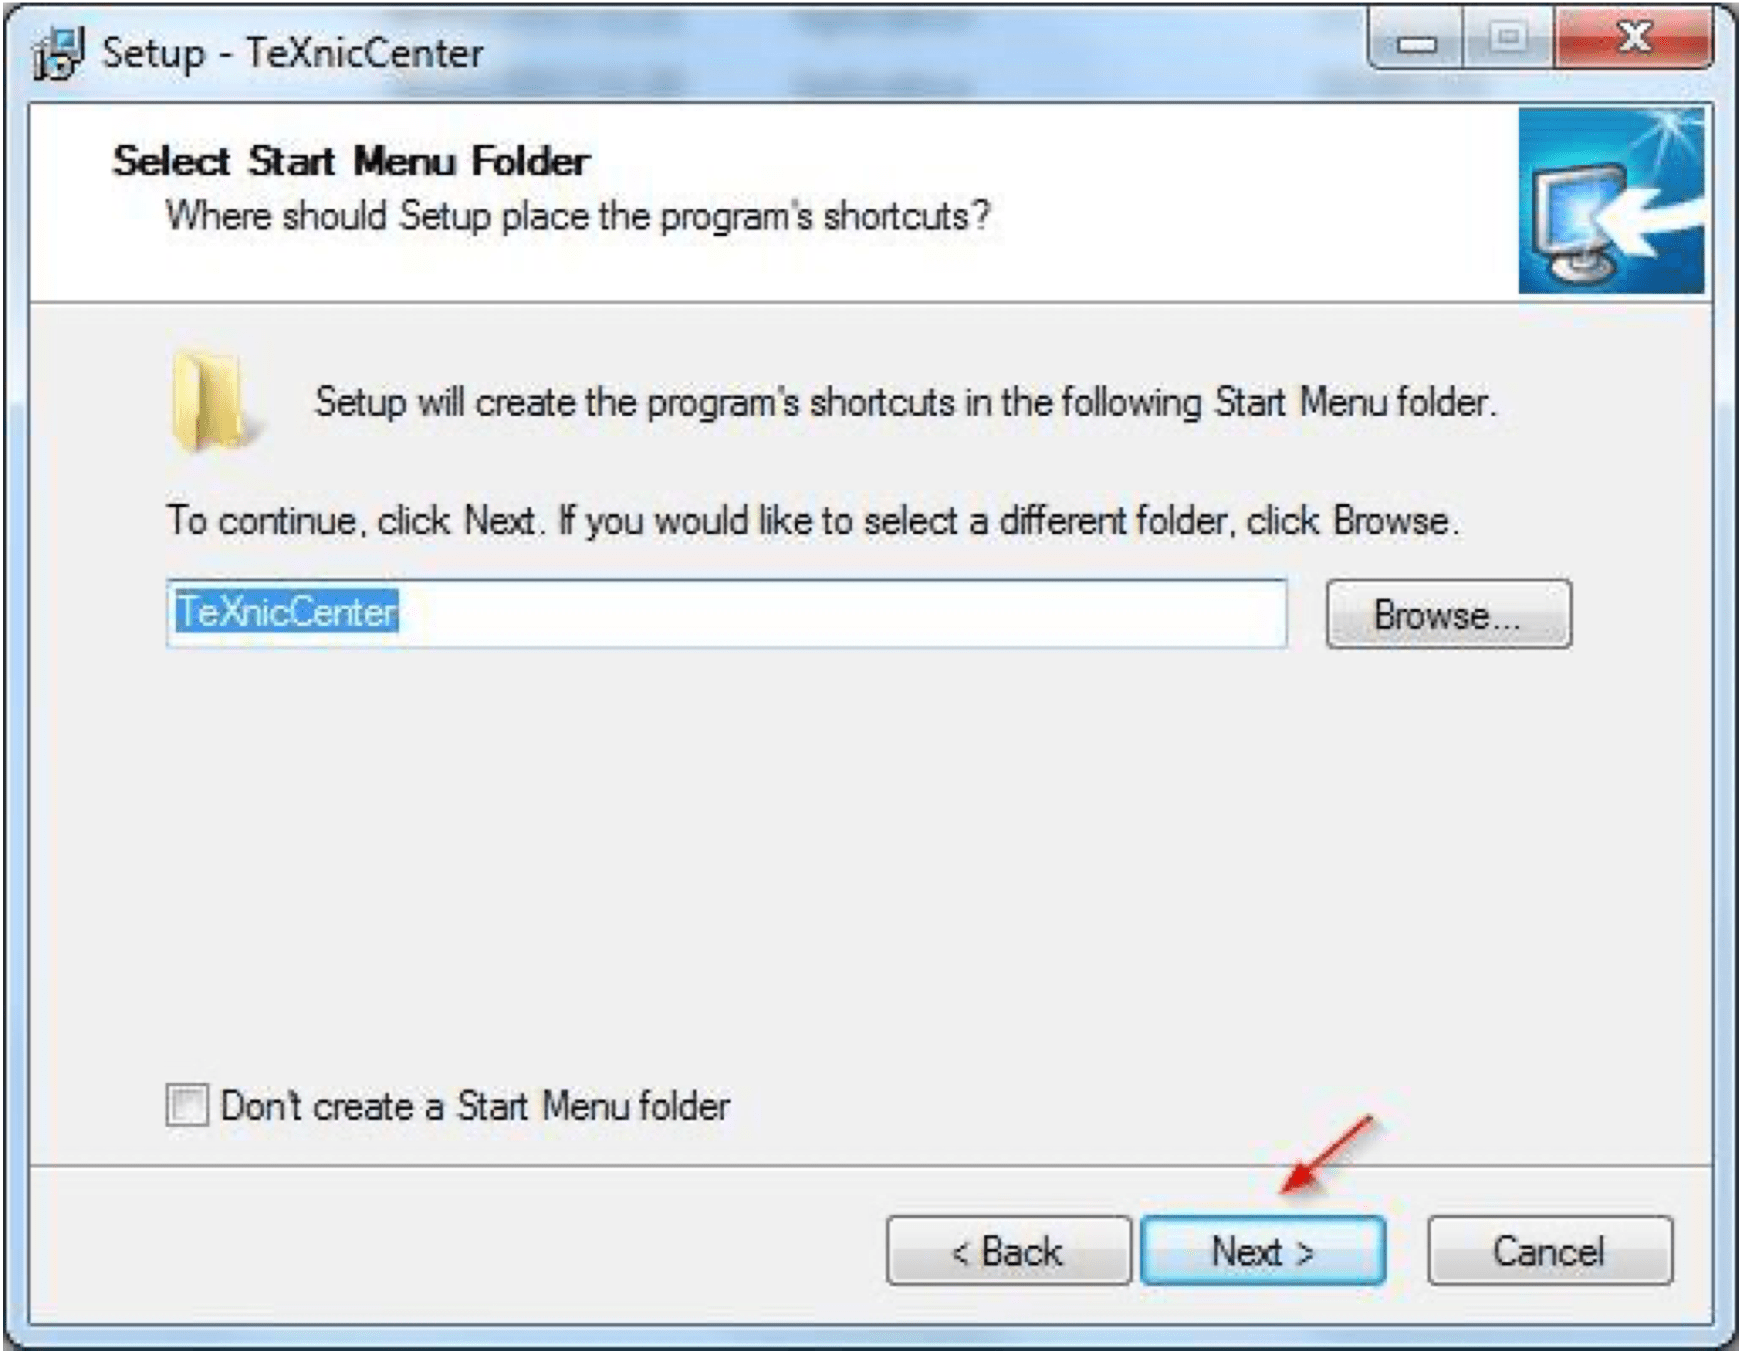
\includegraphics[width=0.6\textwidth]{./fig/texniccenter07}
  \caption{Instalação do TeXnicCenter - Quinta tela.}
  \fontefig{\cite{texnic}}
\end{figure}
\item Serão exibidas as opções para a criação de ícones adicionais para acesso ao software, apenas clique em \textbf{Next} para continuar.
\begin{figure}[H]
  \centering
  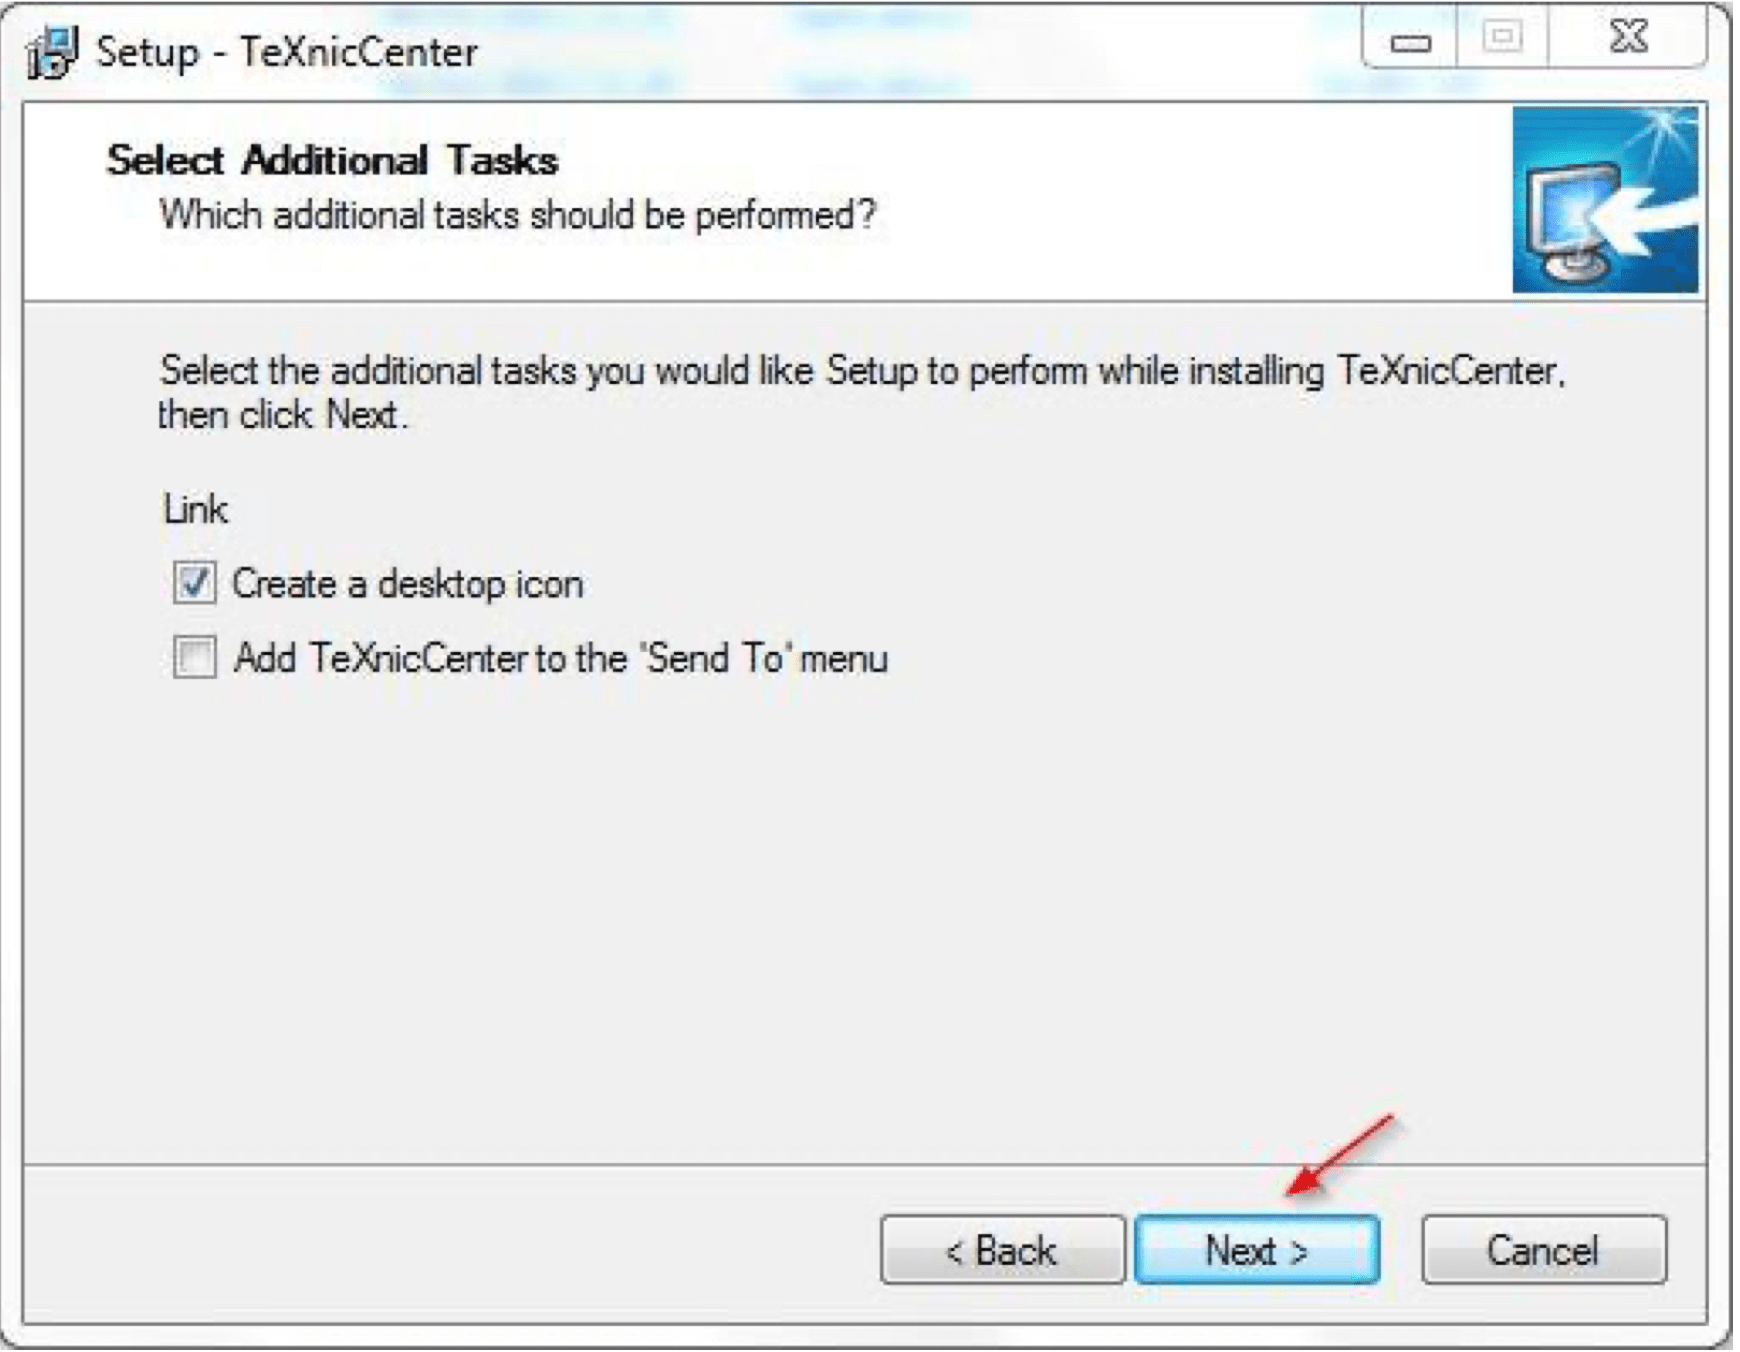
\includegraphics[width=0.6\textwidth]{./fig/texniccenter08}
  \caption{Instalação do TeXnicCenter - Sexta tela.}
  \fontefig{\cite{texnic}}
\end{figure}
\item Um resumo com as opções anteriormente selecionadas será exibido, clique em \textbf{Install} para continuar o processo de instalação do software.
\begin{figure}[H]
  \centering
  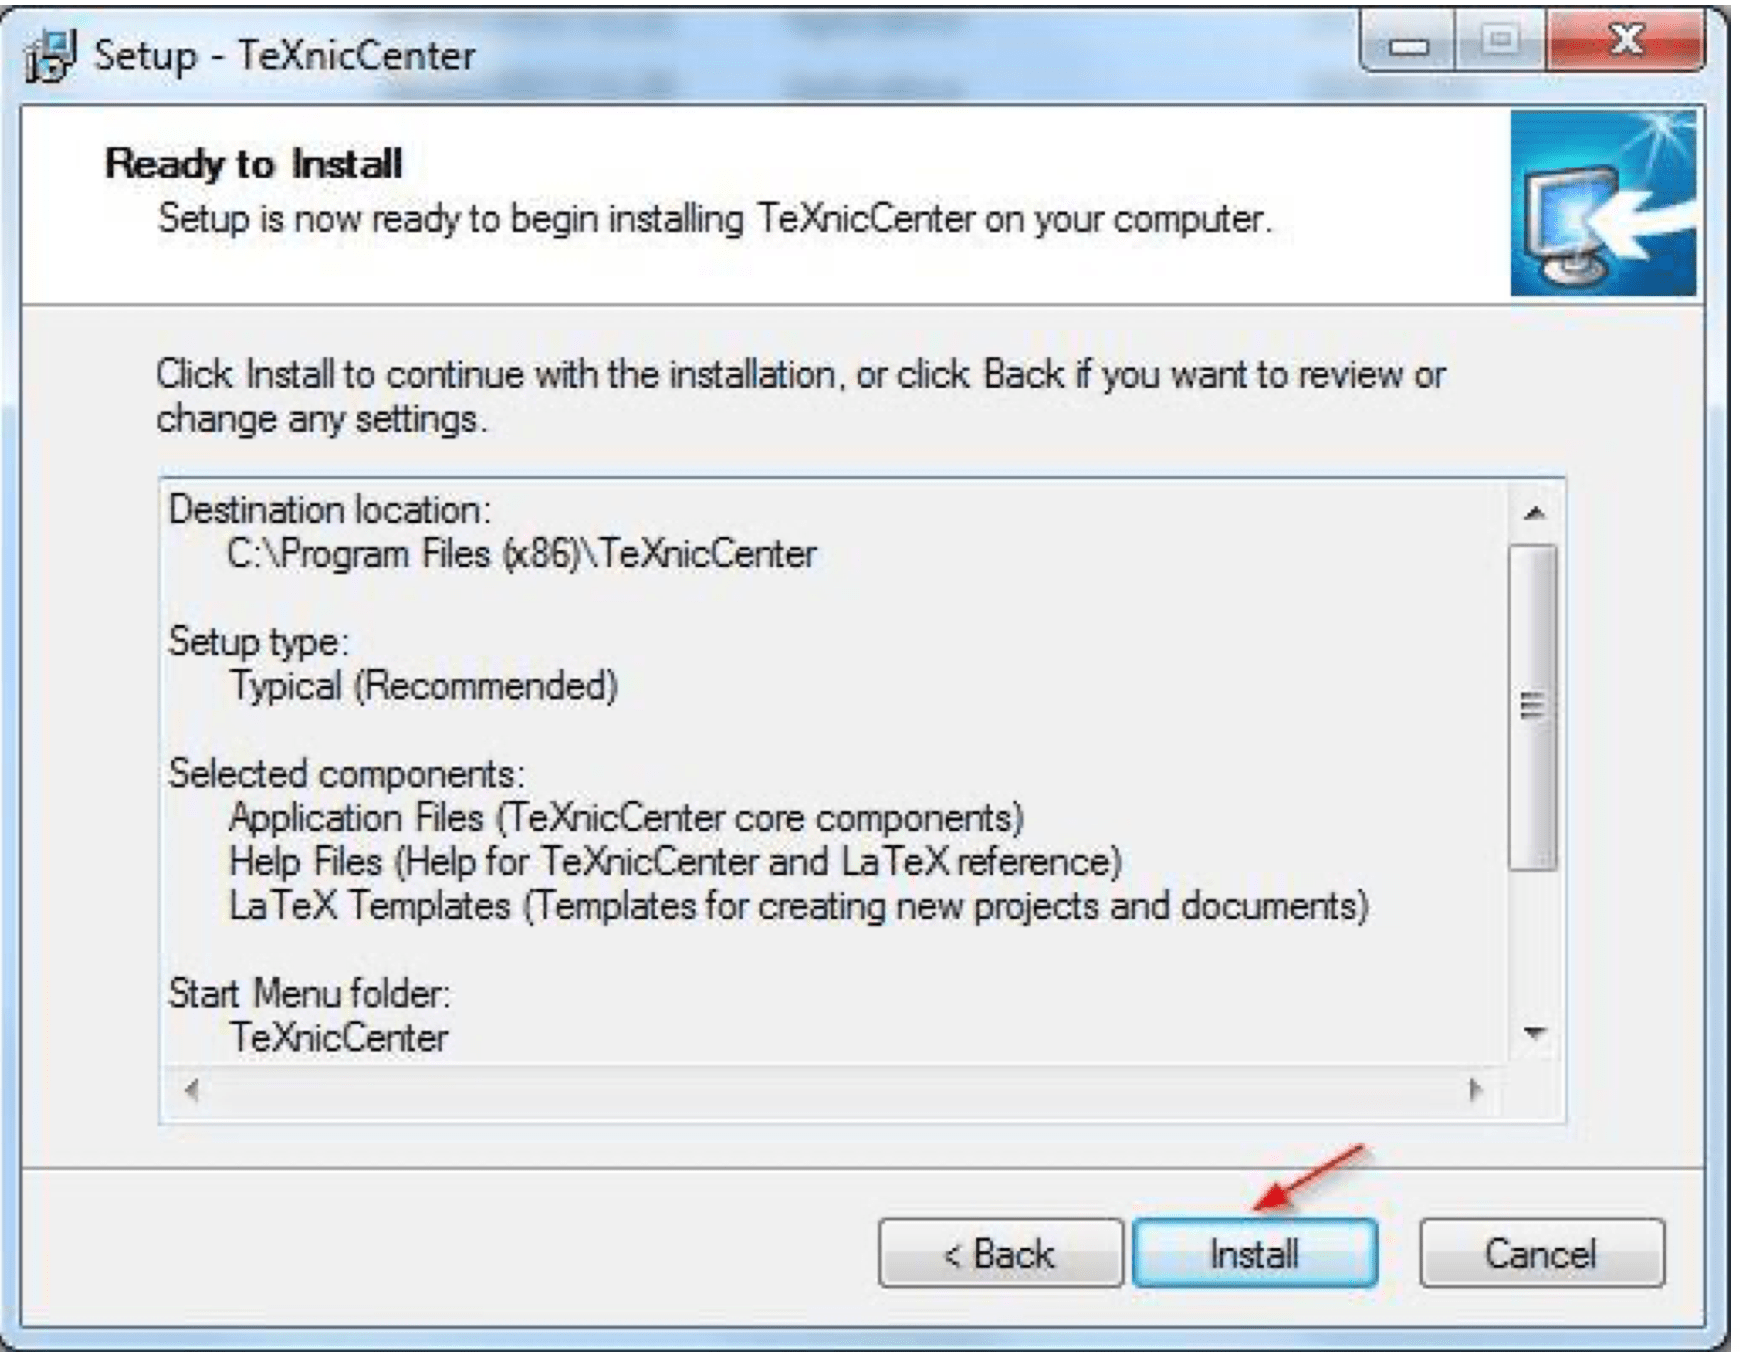
\includegraphics[width=0.6\textwidth]{./fig/texniccenter09}
  \caption{Instalação do TeXnicCenter - Sétima tela.}
  \fontefig{\cite{texnic}}
\end{figure}
\item Apenas aguarde a finalização do processo de instalação.
\begin{figure}[H]
  \centering
  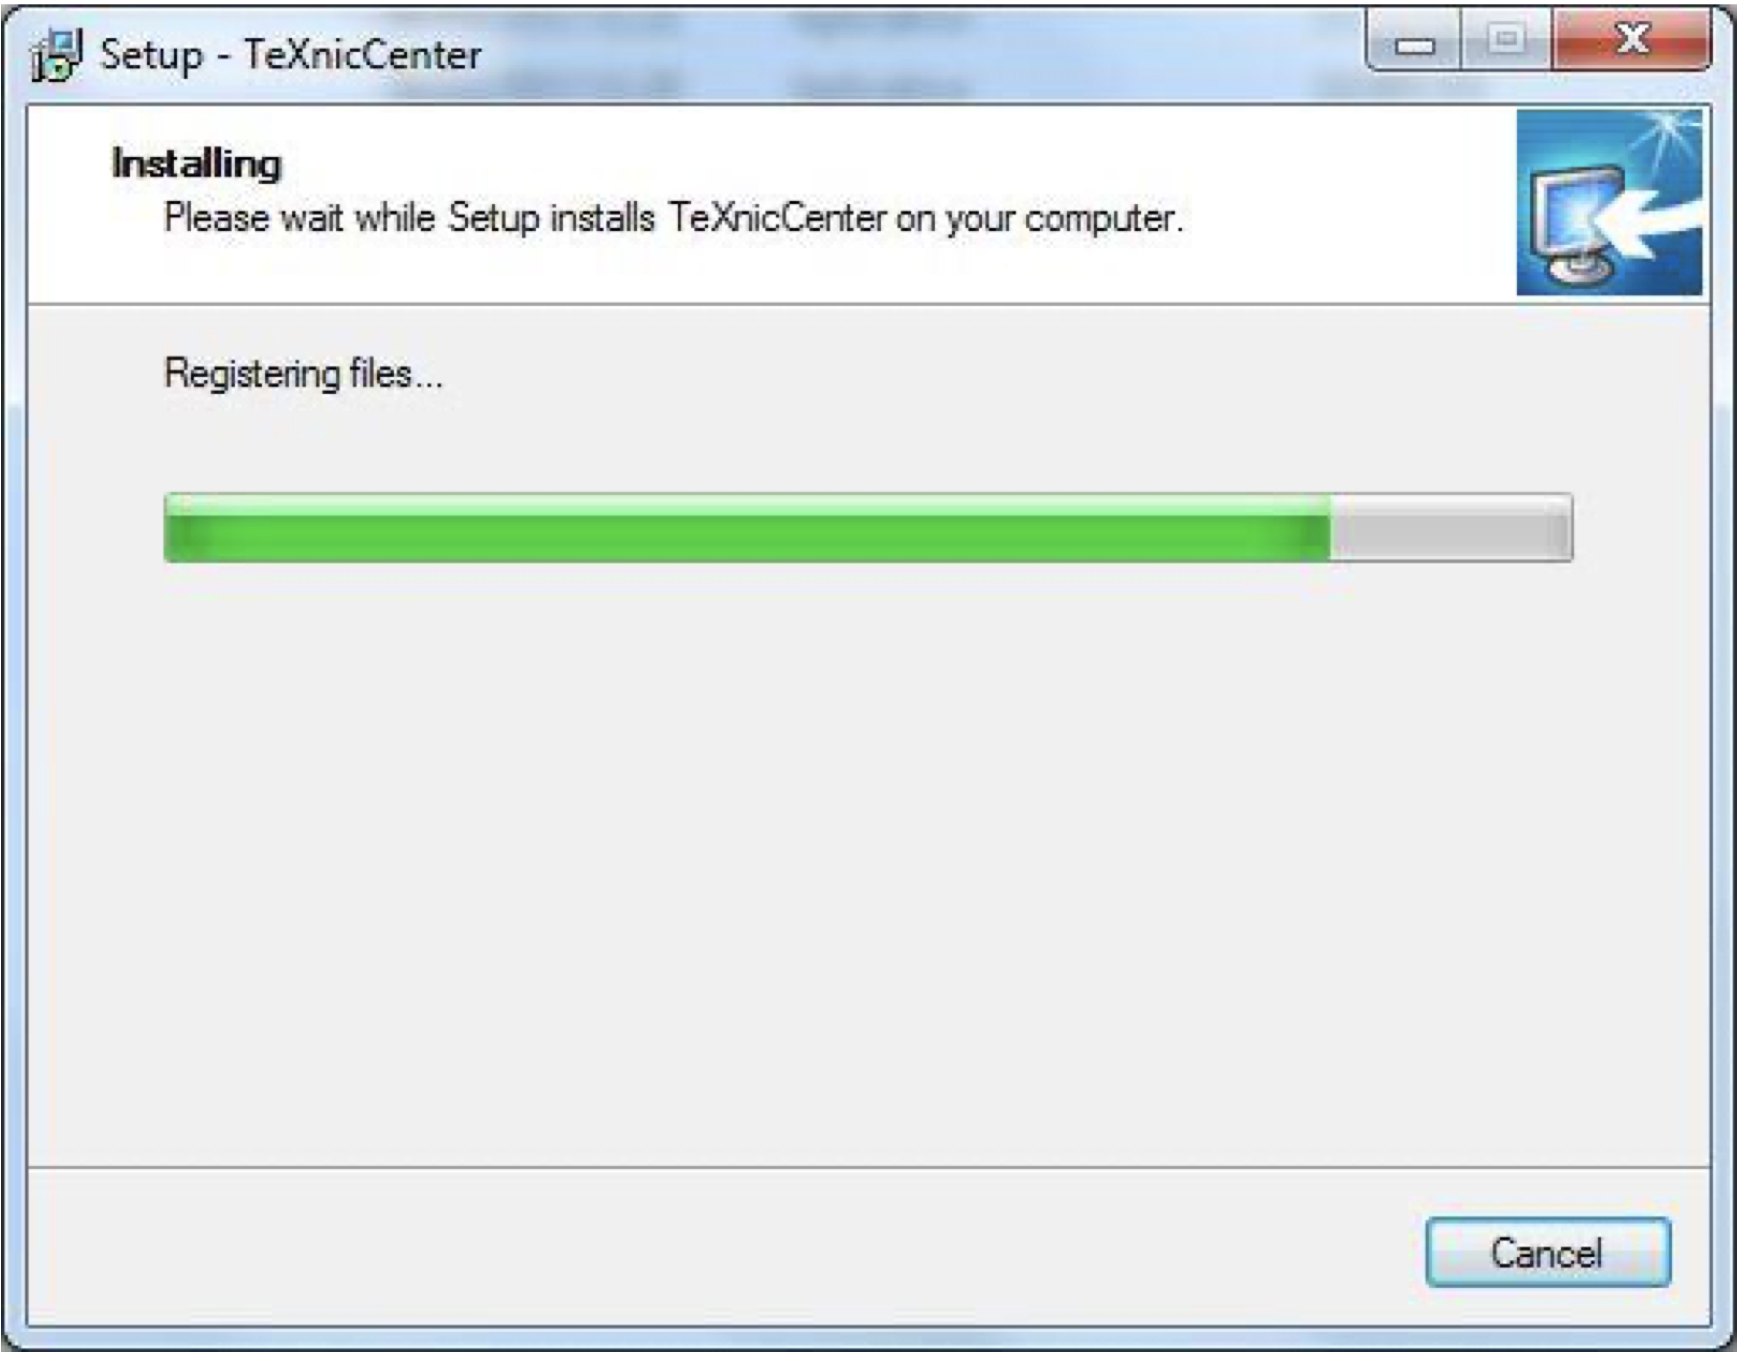
\includegraphics[width=0.6\textwidth]{./fig/texniccenter10}
  \caption{Instalação do TeXnicCenter - Oitava tela.}
  \fontefig{\cite{texnic}}
\end{figure}
\item Para finalizar o processo de instalação clique no botão \textbf{Finish}.
\begin{figure}[H]
  \centering
  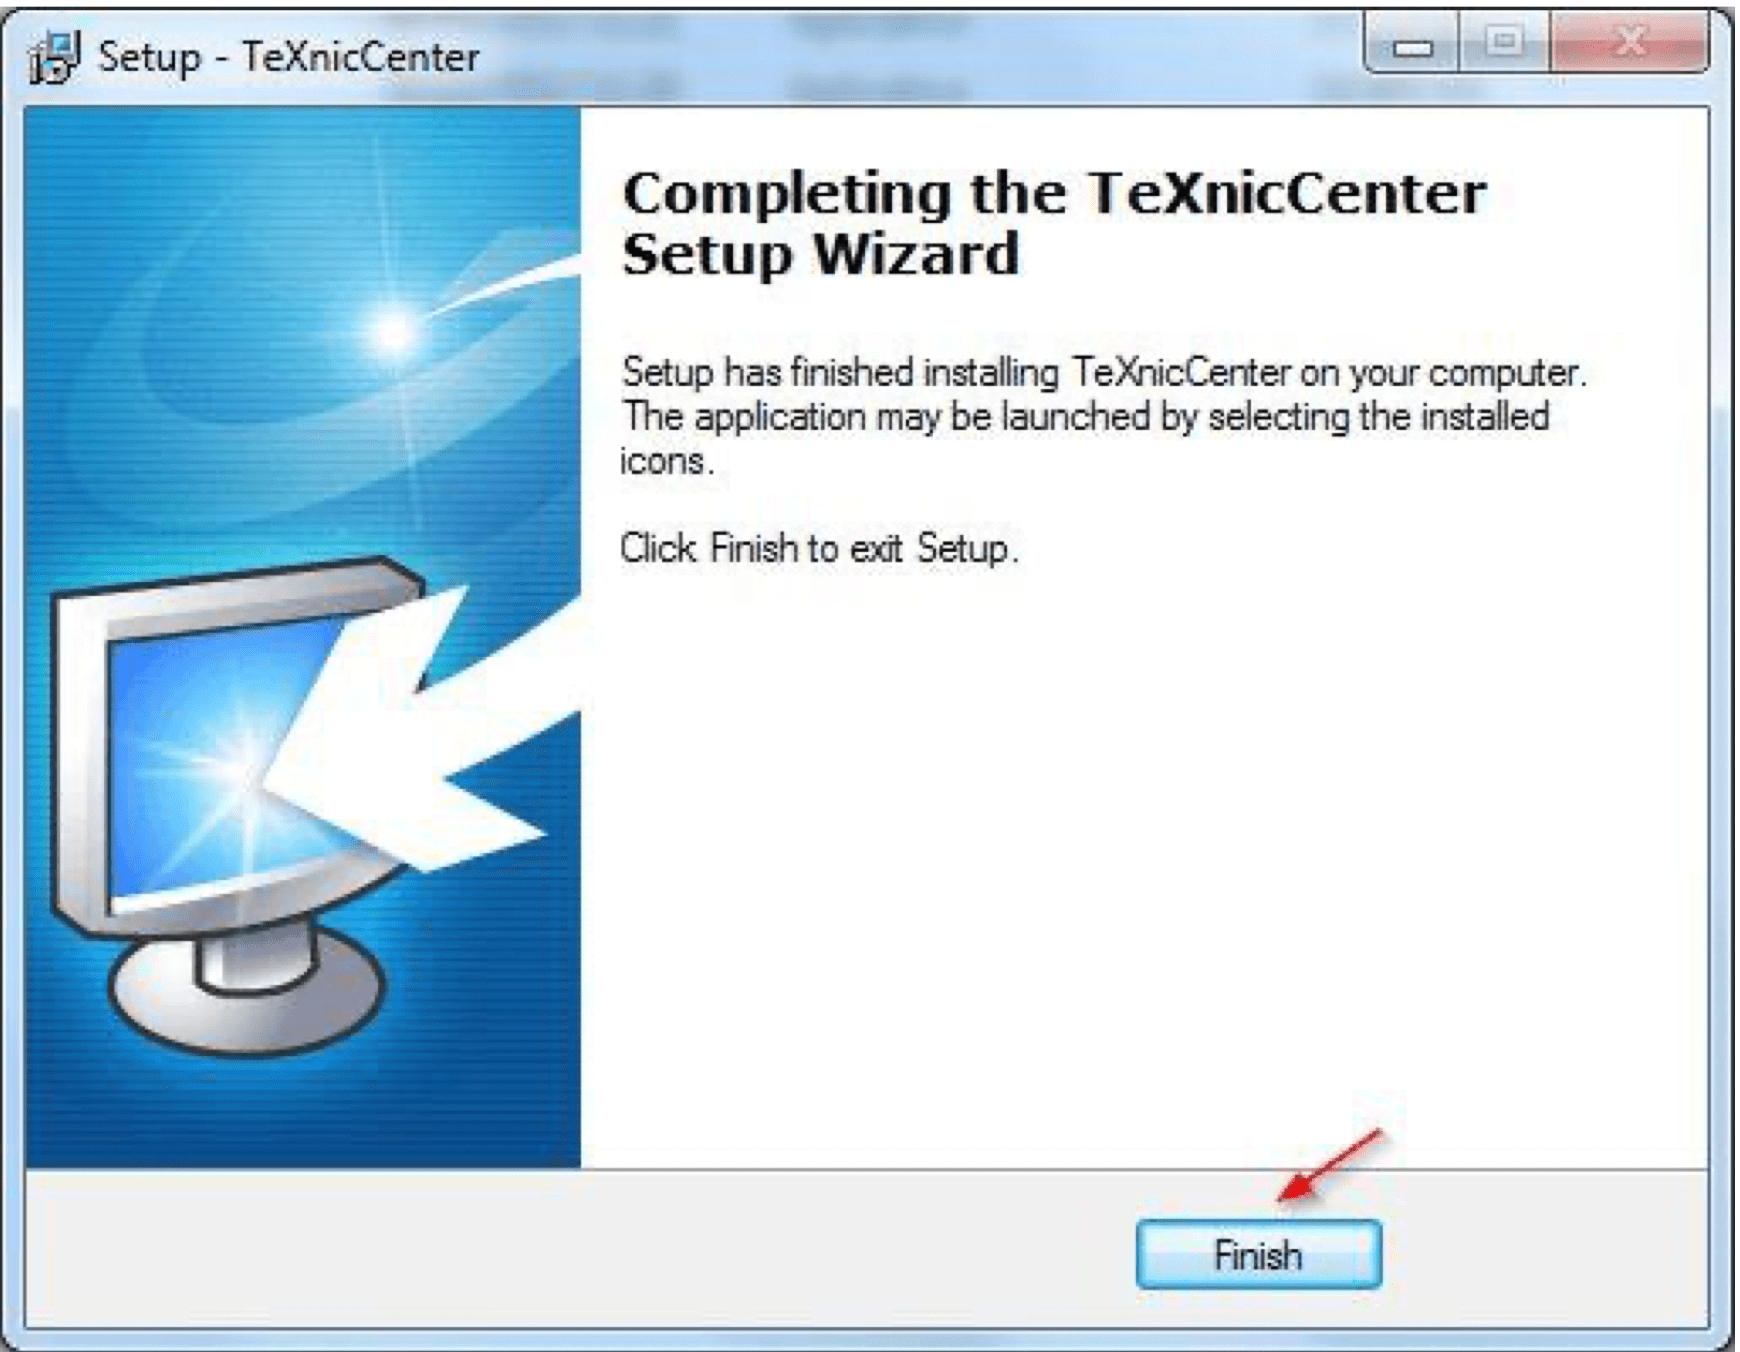
\includegraphics[width=0.6\textwidth]{./fig/texniccenter11}
  \caption{Instalação do TeXnicCenter - Nona tela.}
  \fontefig{\cite{texnic}}
\end{figure}
\end{enumerate}

O TeXnicCenter está instalado em seu computador, agora será necessário configurar o software em sua primeira execução. Os passos a seguir ilustram como deve ser feita a configuração inicial do TeXnicCenter.

\begin{enumerate}
\item Abra o programa TeXnicCenter, ao abrir será exibida uma janela de dicas de uso, clique no botão \textbf{Close} para fechar a janela.
\begin{figure}[H]
  \centering
  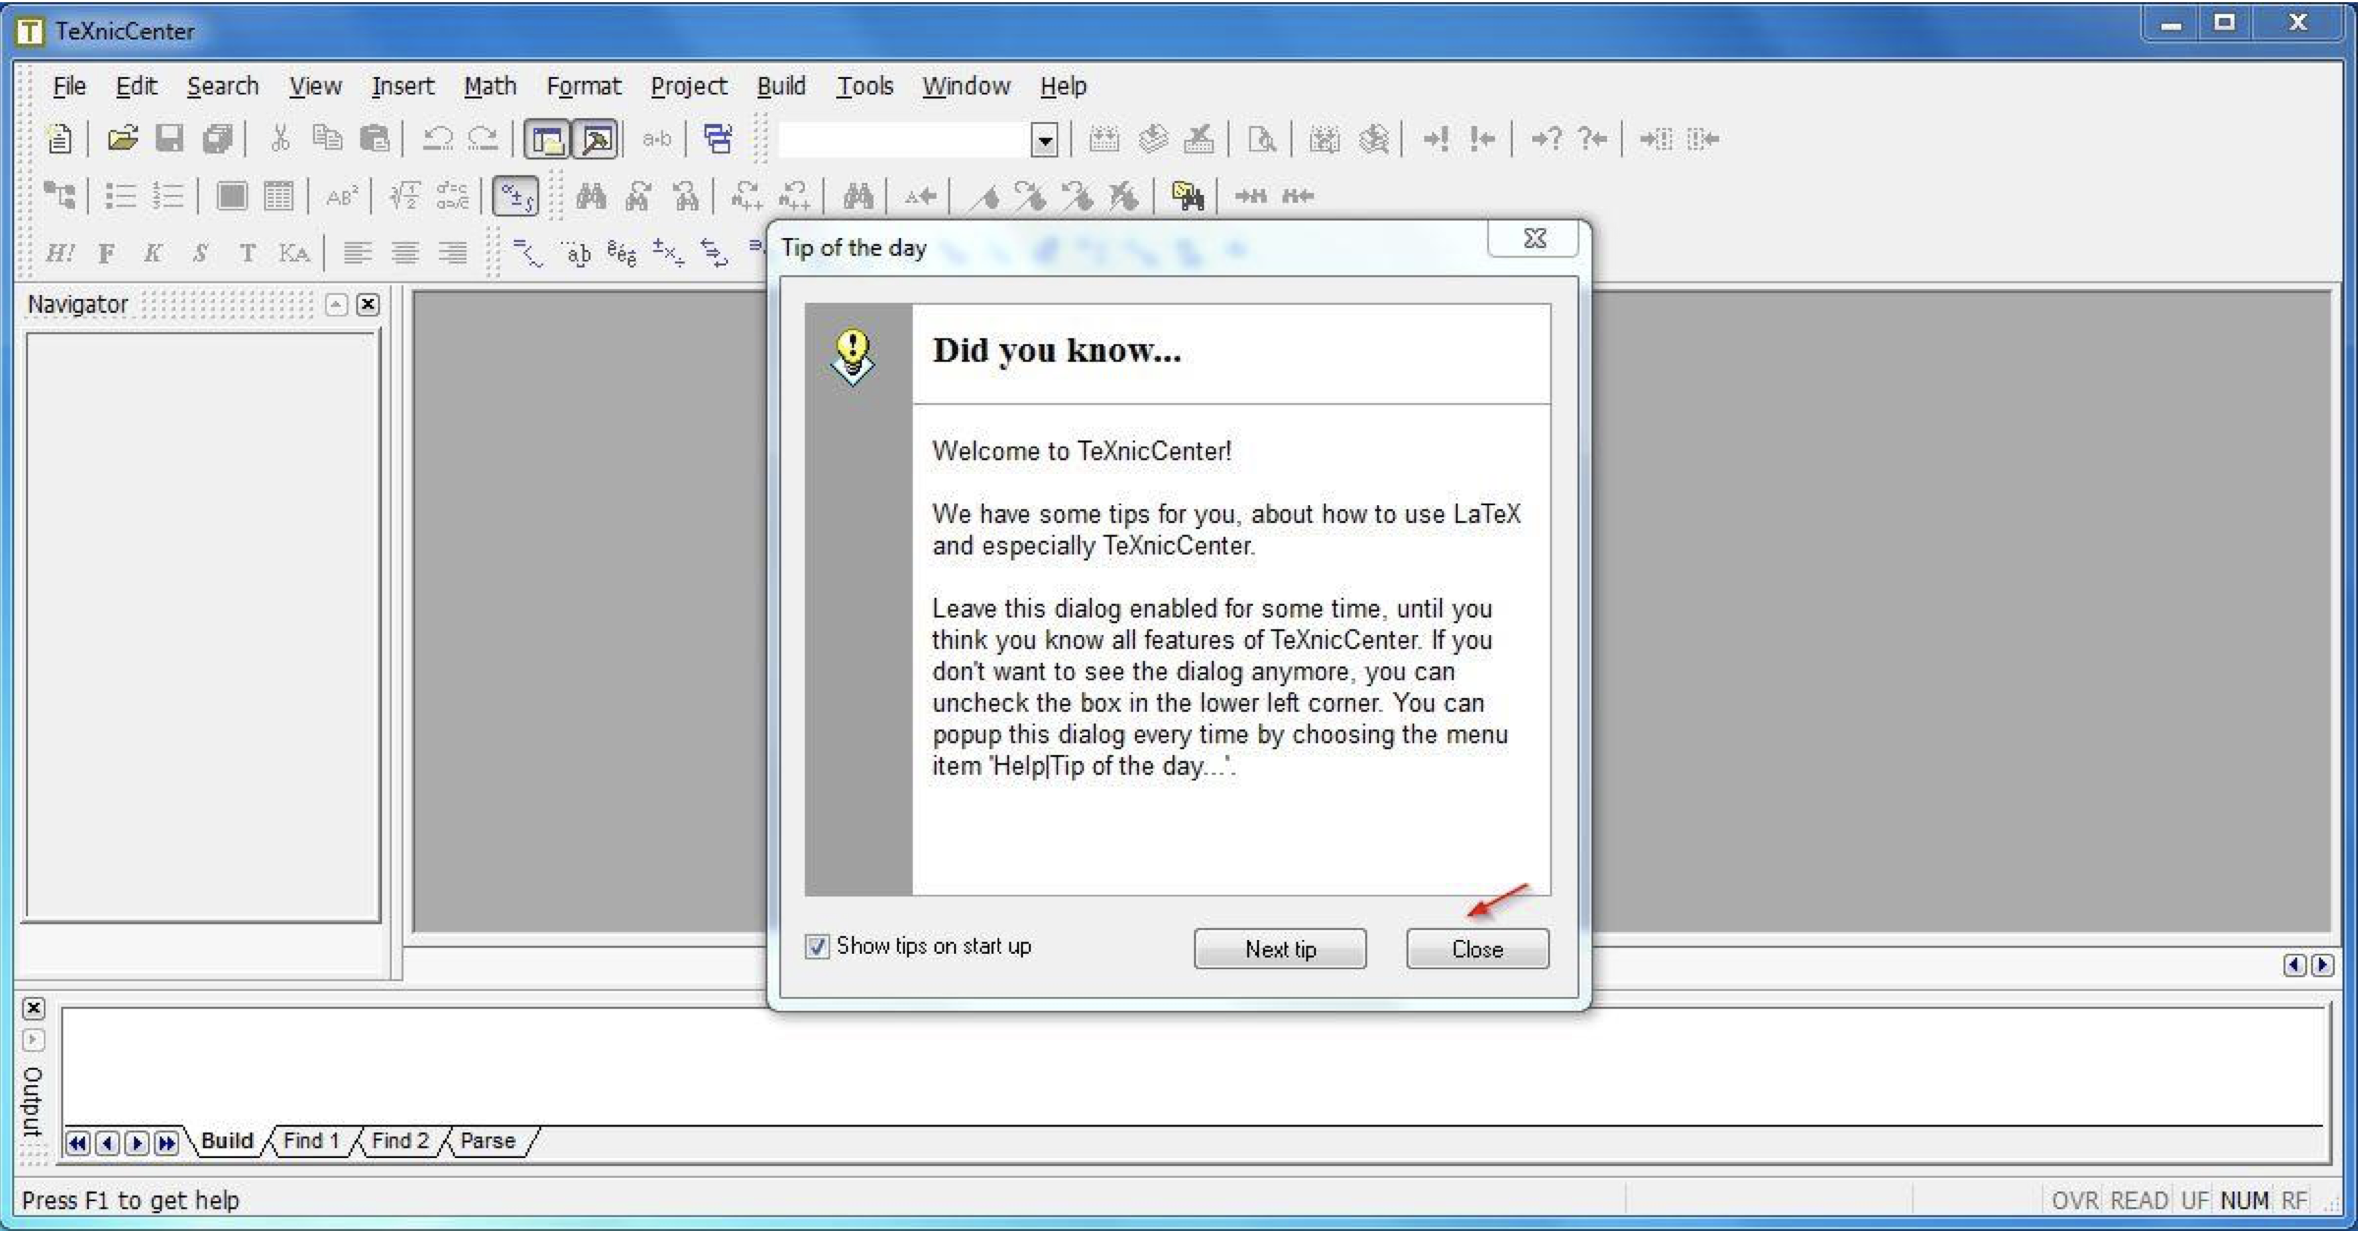
\includegraphics[width=1.0\textwidth]{./fig/texniccenter12}
  \caption{Configuração do TeXnicCenter - Primeira tela.}
  \fontefig{\cite{texnic}}
\end{figure}
\item A janela de configuração inicial do software será exibida clique no botão \textbf{Avançar} para iniciar o processo.
\begin{figure}[H]
  \centering
  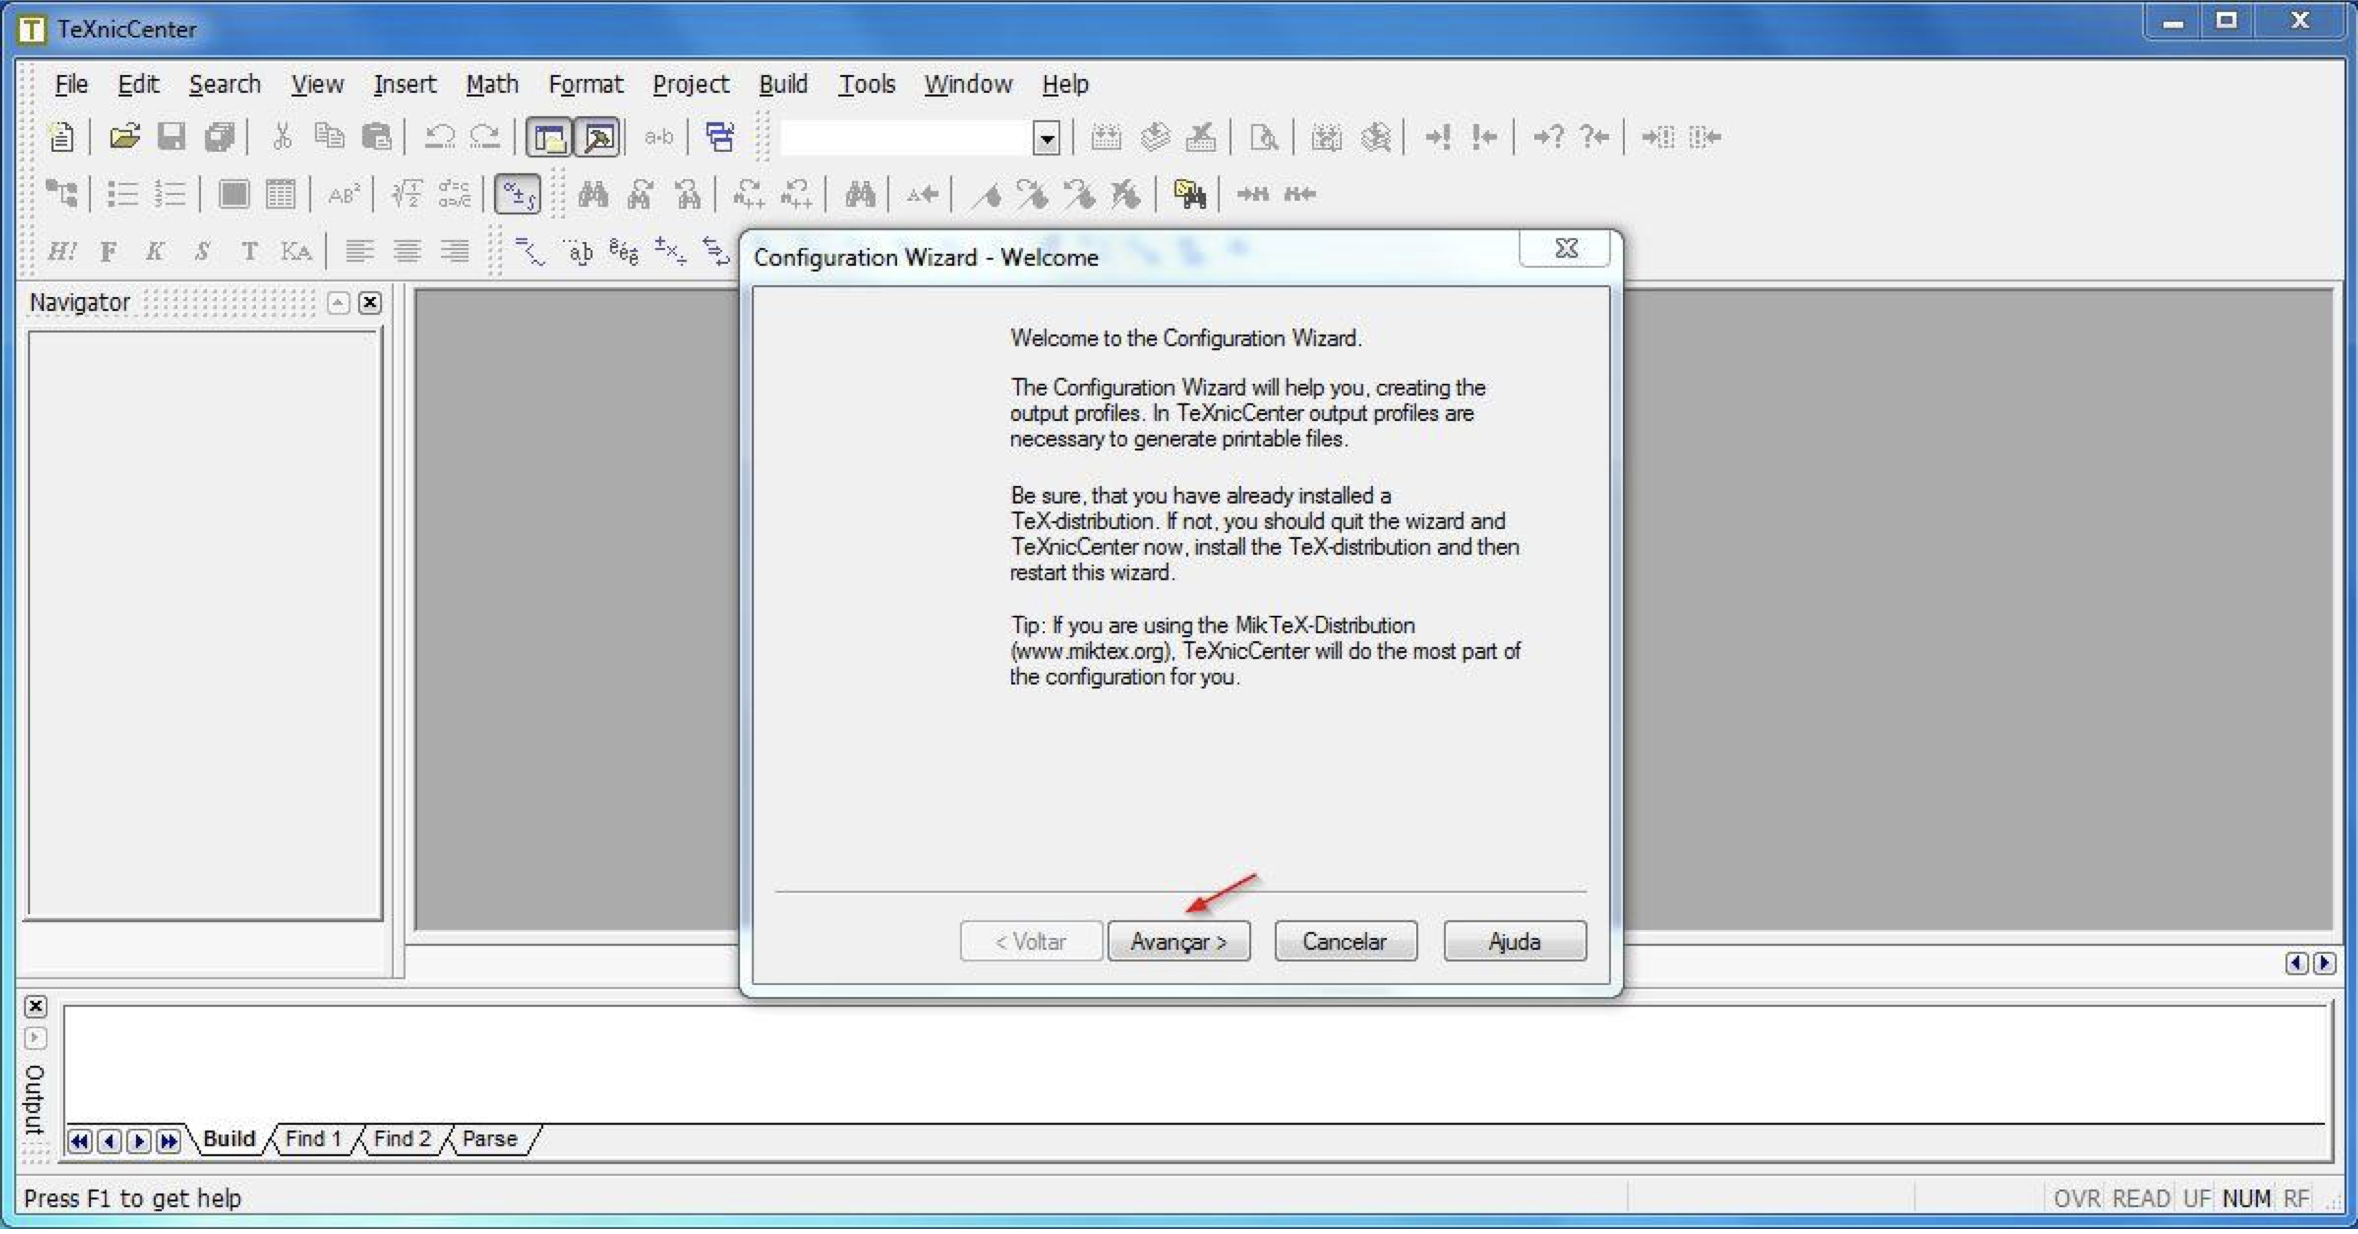
\includegraphics[width=1.0\textwidth]{./fig/texniccenter13}
  \caption{Configuração do TeXnicCenter - Segunda tela.}
  \fontefig{\cite{texnic}}
\end{figure}
\item Na janela exibida será necessário informar na caixa em branco o local onde estão os executáveis do MiKTeX, para isto localize a pasta onde foi instalado o MikTeX (conforme anotado em seu processo de instalação, neste tutorial é a pasta: \aspas{C:$\backslash$Program Files (x86)$\backslash$MiKTeX 2.9}, mas pode variar dependendo da versão do Windows utilizado), dentro da pasta do MikTeX localize a pasta \textbf{miktex} e dentro dela a pasta \textbf{bin}.
\begin{figure}[H]
  \centering
  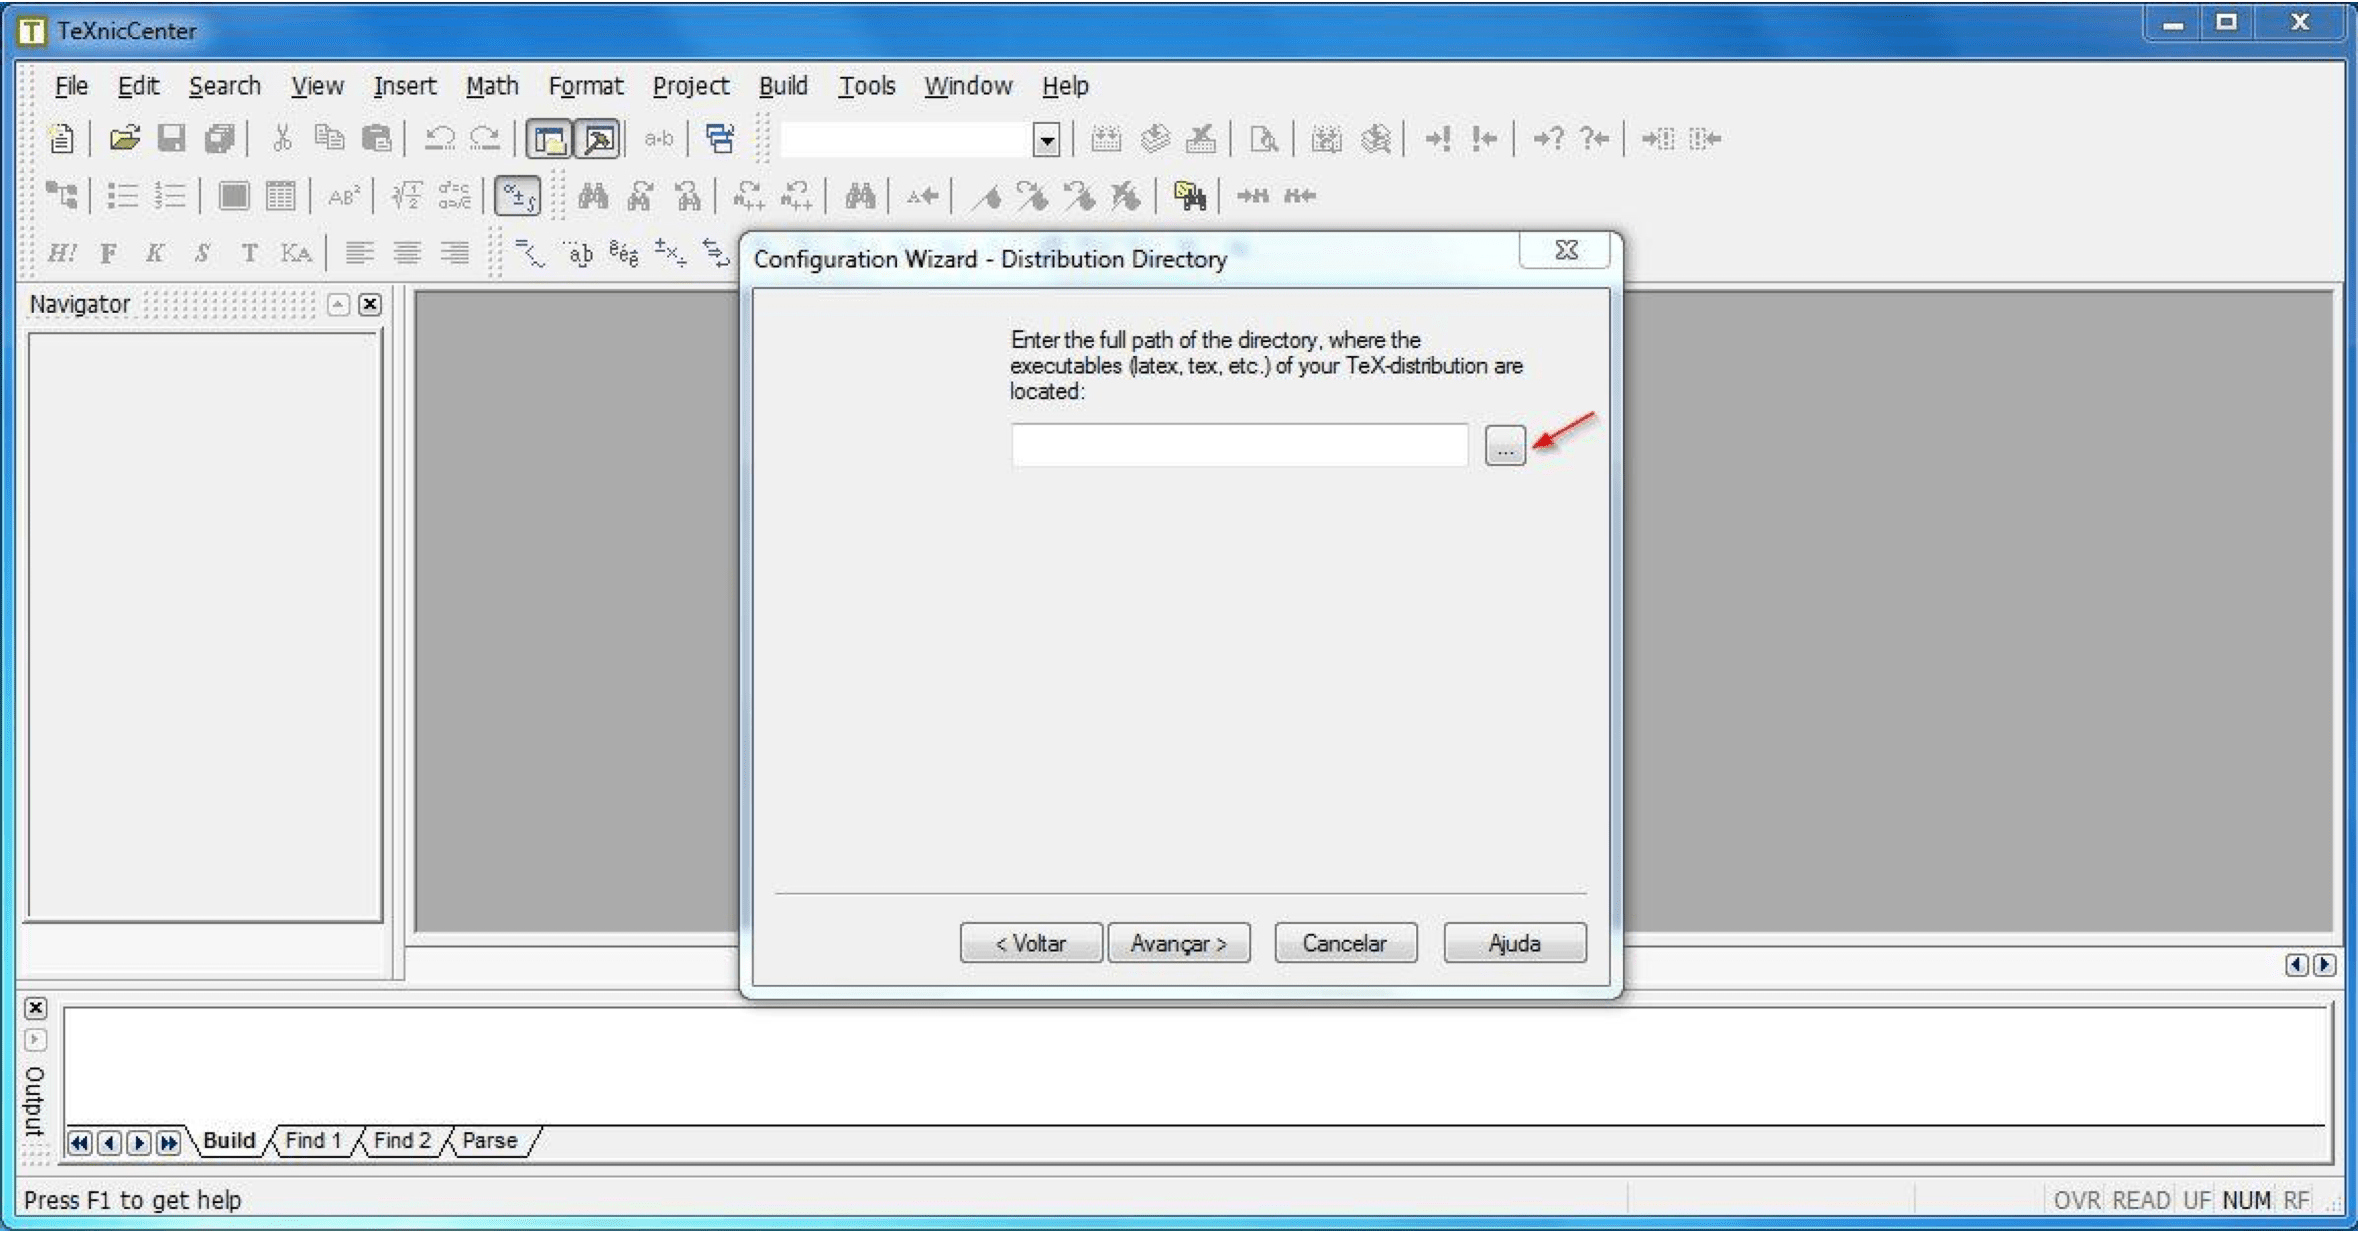
\includegraphics[width=1.0\textwidth]{./fig/texniccenter14}
  \caption{Configuração do TeXnicCenter - Terceira tela.}
  \fontefig{\cite{texnic}}
\end{figure}
Você pode copiar e colar o local dos executáveis do MiKTeX (neste tutorial é: \aspas{C:$\backslash$Program Files (x86)$\backslash$MiKTeX 2. 9$\backslash$miktex$\backslash$bin}, mas pode variar dependendo da versão do Windows utilizado) na caixa em branco ou pode procurar a pasta utilizando o botão \aspas{...}.
\item Após selecionada a pasta dos executáveis do MiKTeX, clique no botão \textbf{Avançar}.
\begin{figure}[H]
  \centering
  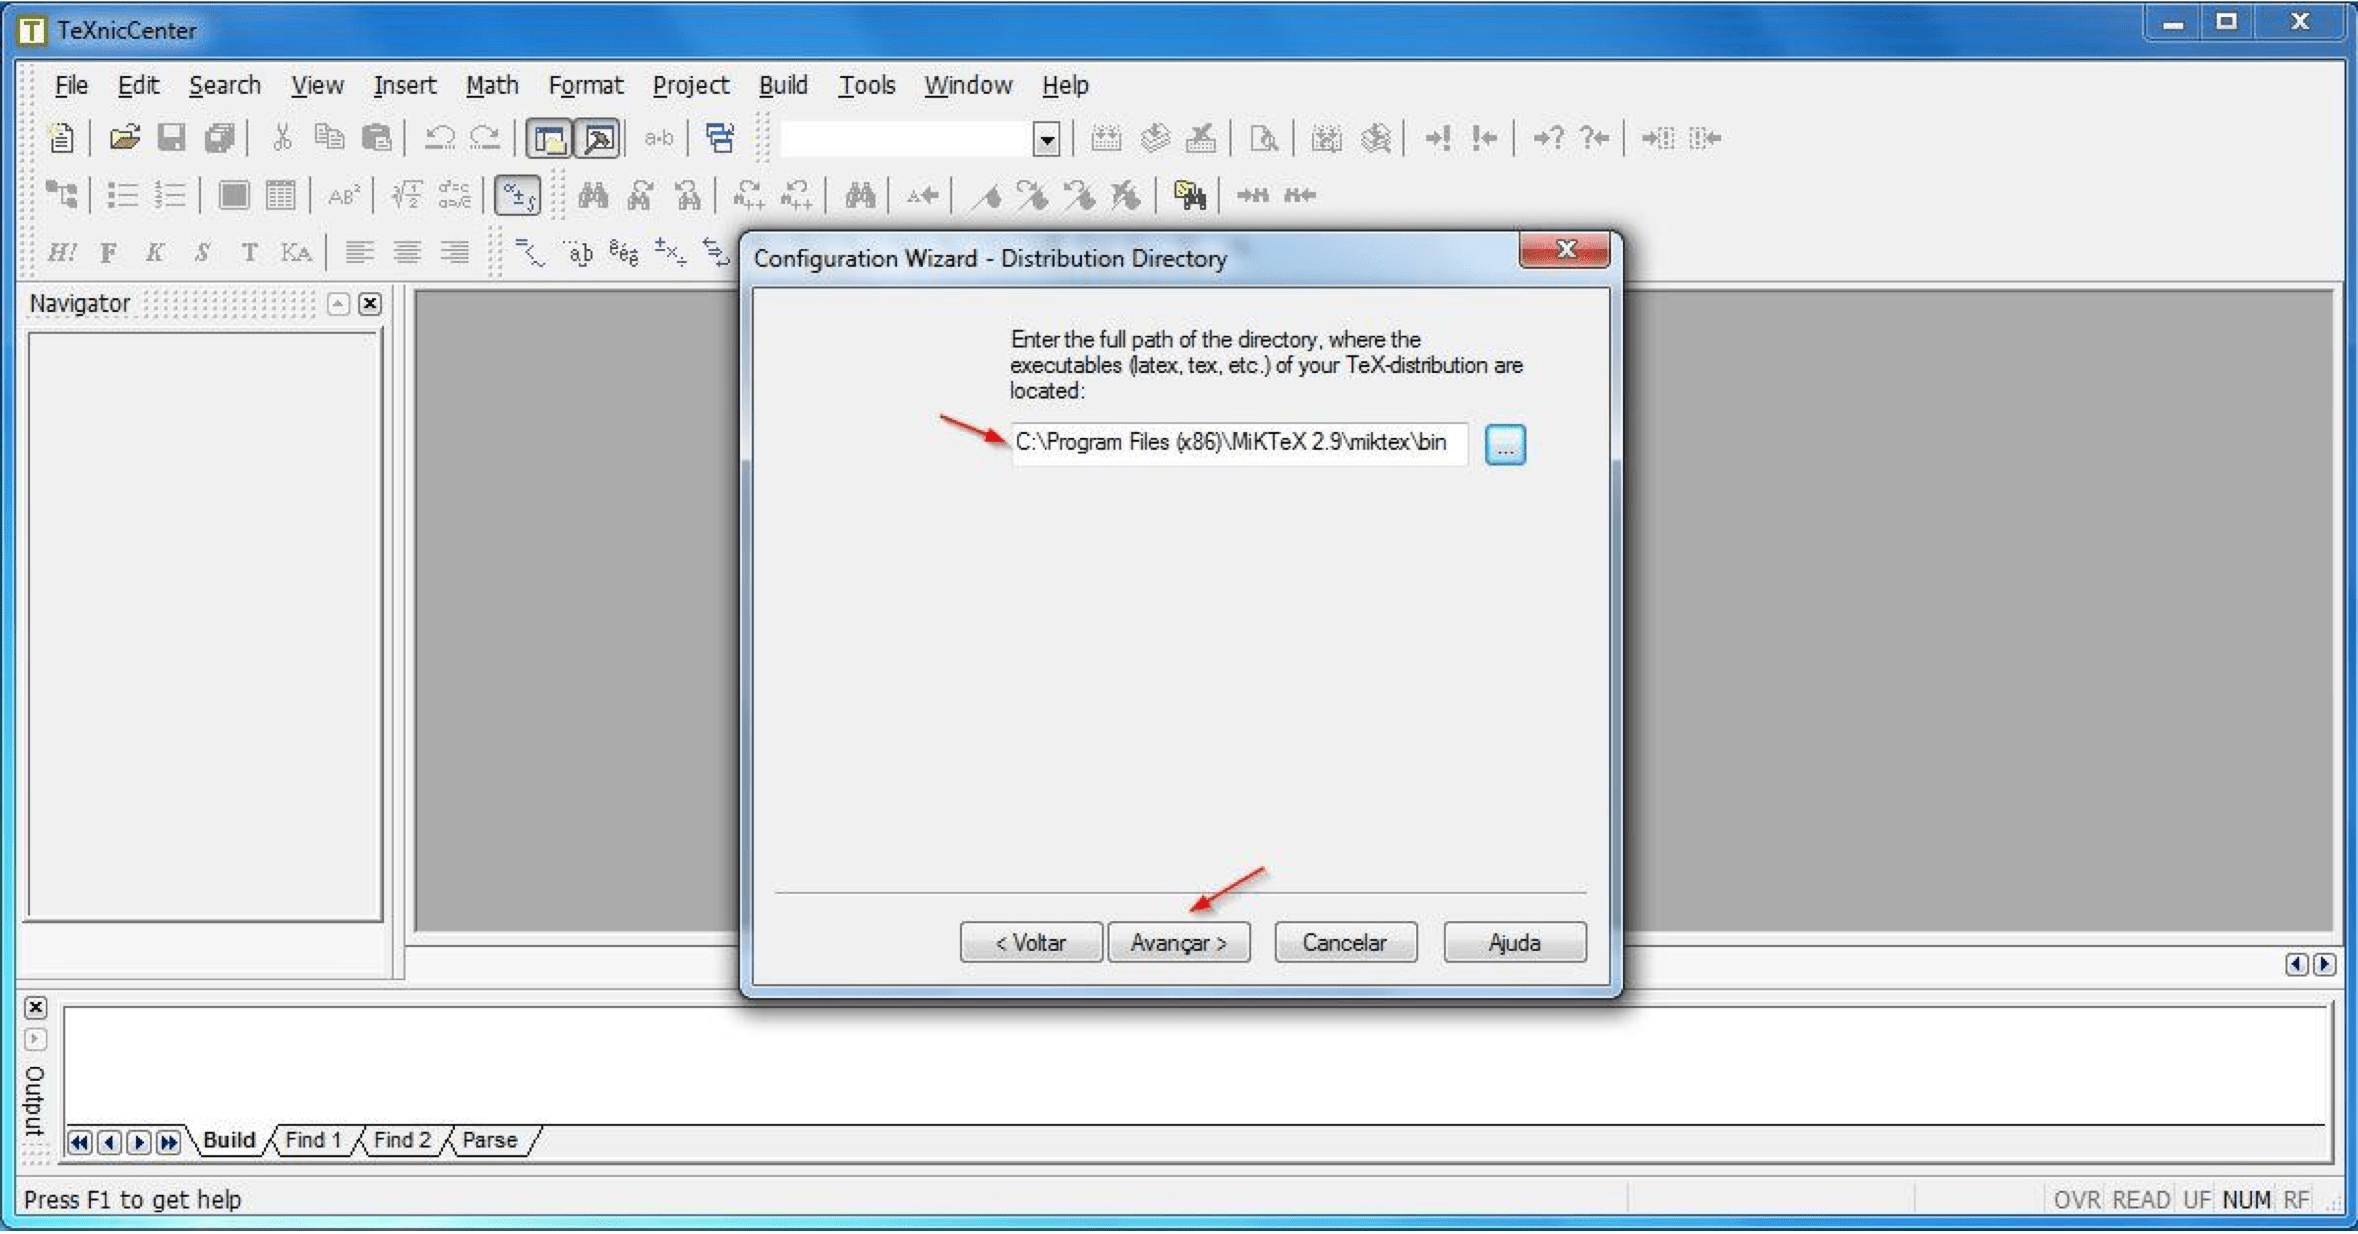
\includegraphics[width=1.0\textwidth]{./fig/texniccenter15}
  \caption{Configuração do TeXnicCenter - Quarta tela.}
  \fontefig{\cite{texnic}}
\end{figure}
\item Serão exibidas as opções para configuração do PostScript que são opcionais, clique apenas no botão \textbf{Avançar}.
\begin{figure}[H]
  \centering
  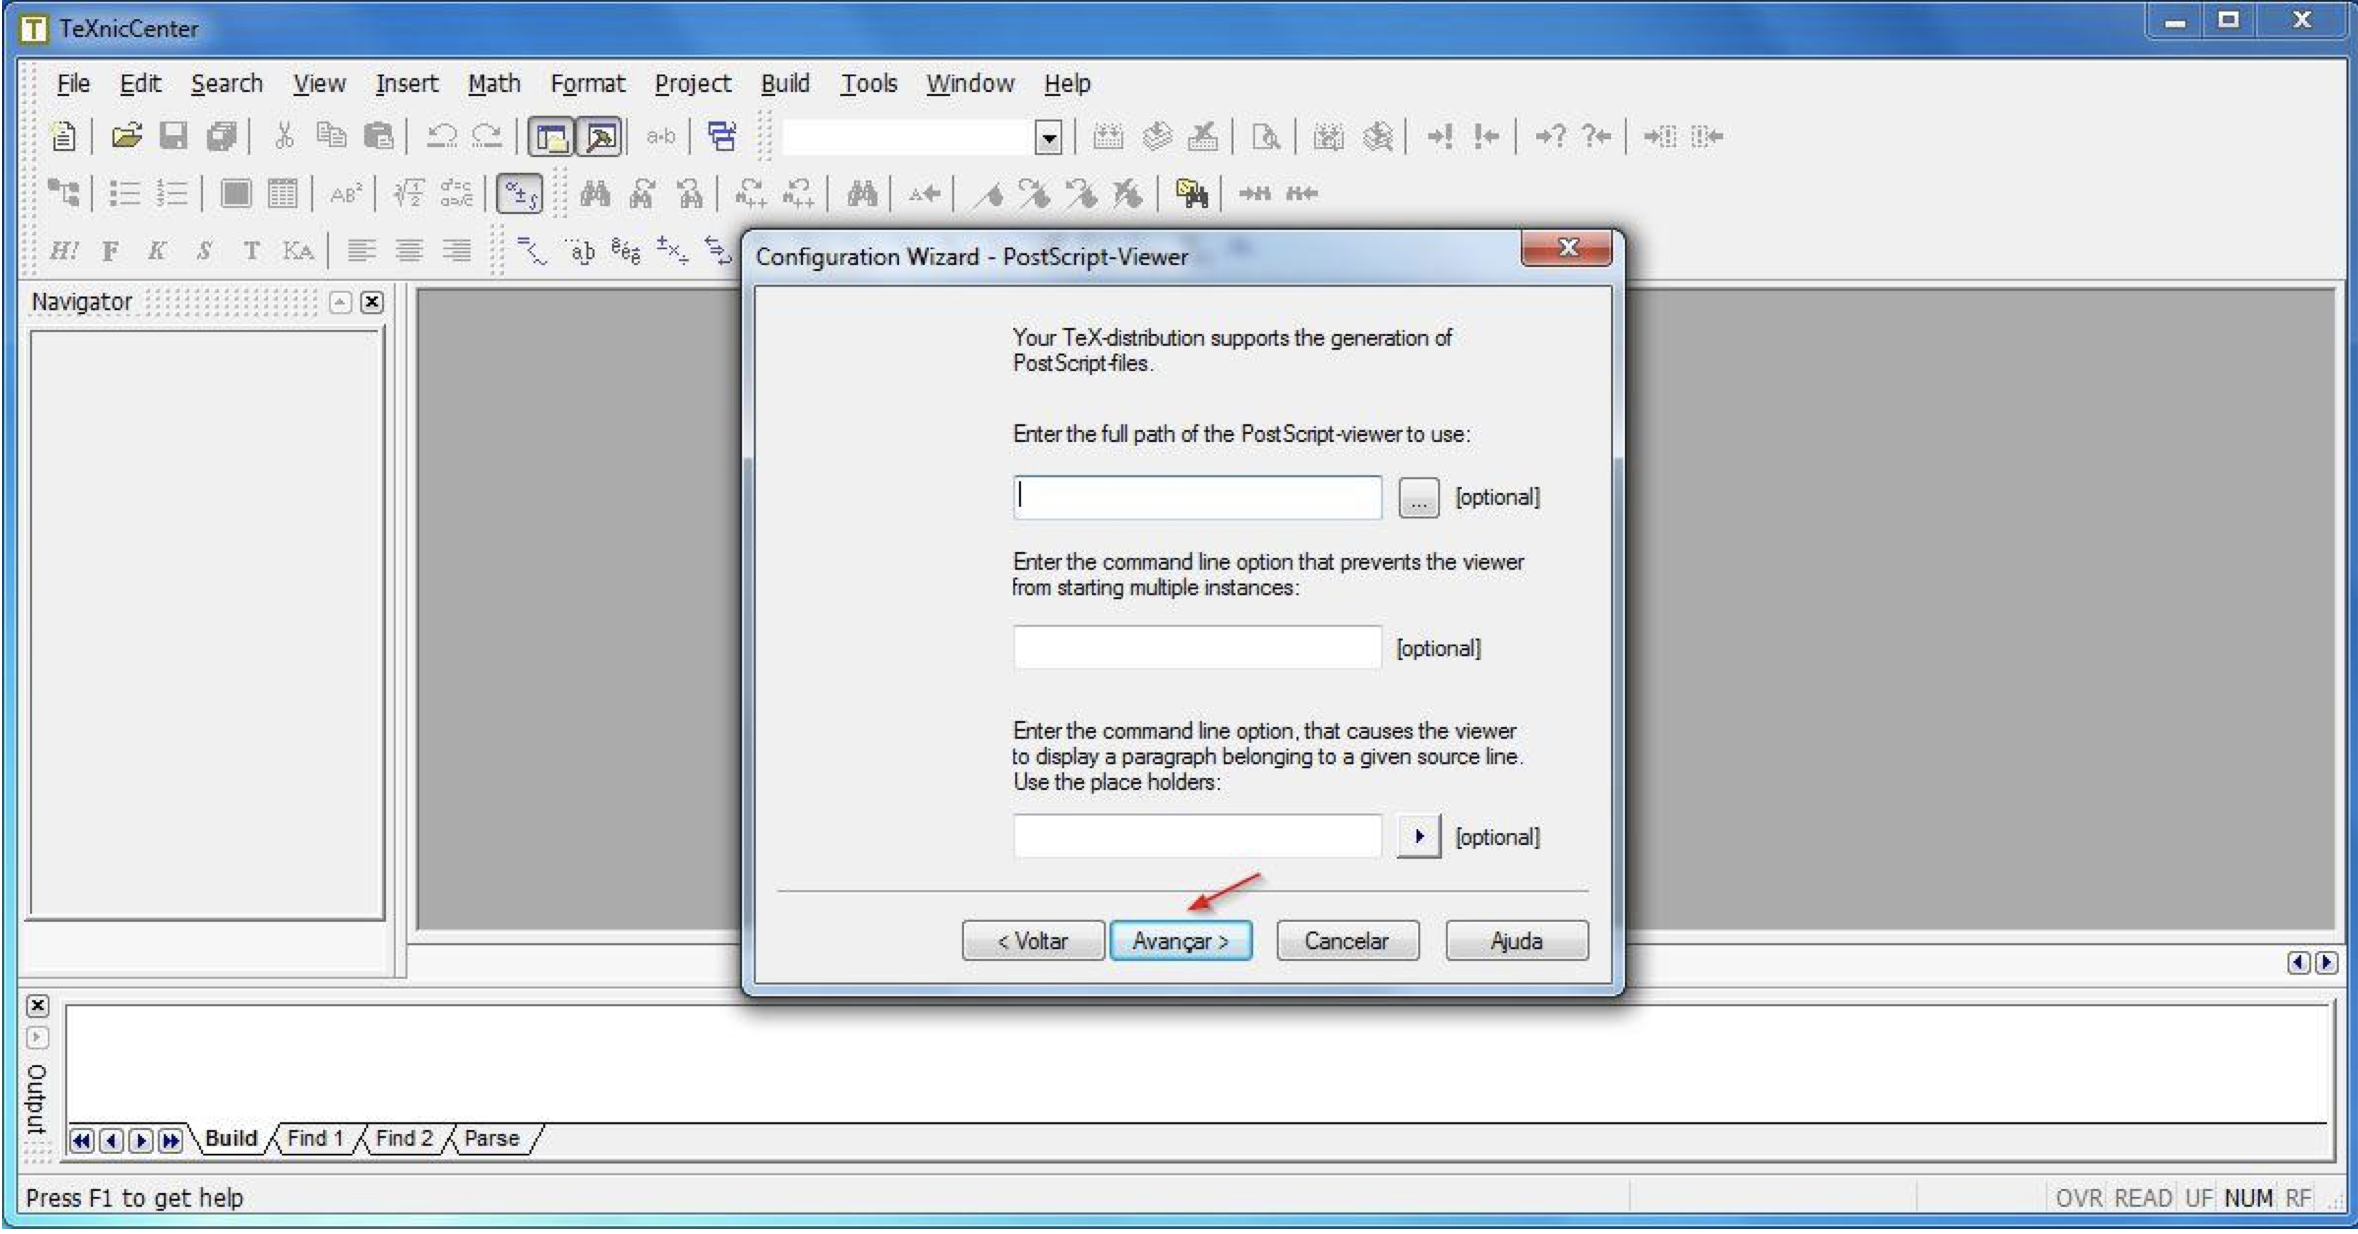
\includegraphics[width=1.0\textwidth]{./fig/texniccenter16}
  \caption{Configuração do TeXnicCenter - Quinta tela.}
  \fontefig{\cite{texnic}}
\end{figure}
\item Agora serão exibidas as opções de PDF opcionais, apenas clique no botão \textbf{Avançar}.
\begin{figure}[H]
  \centering
  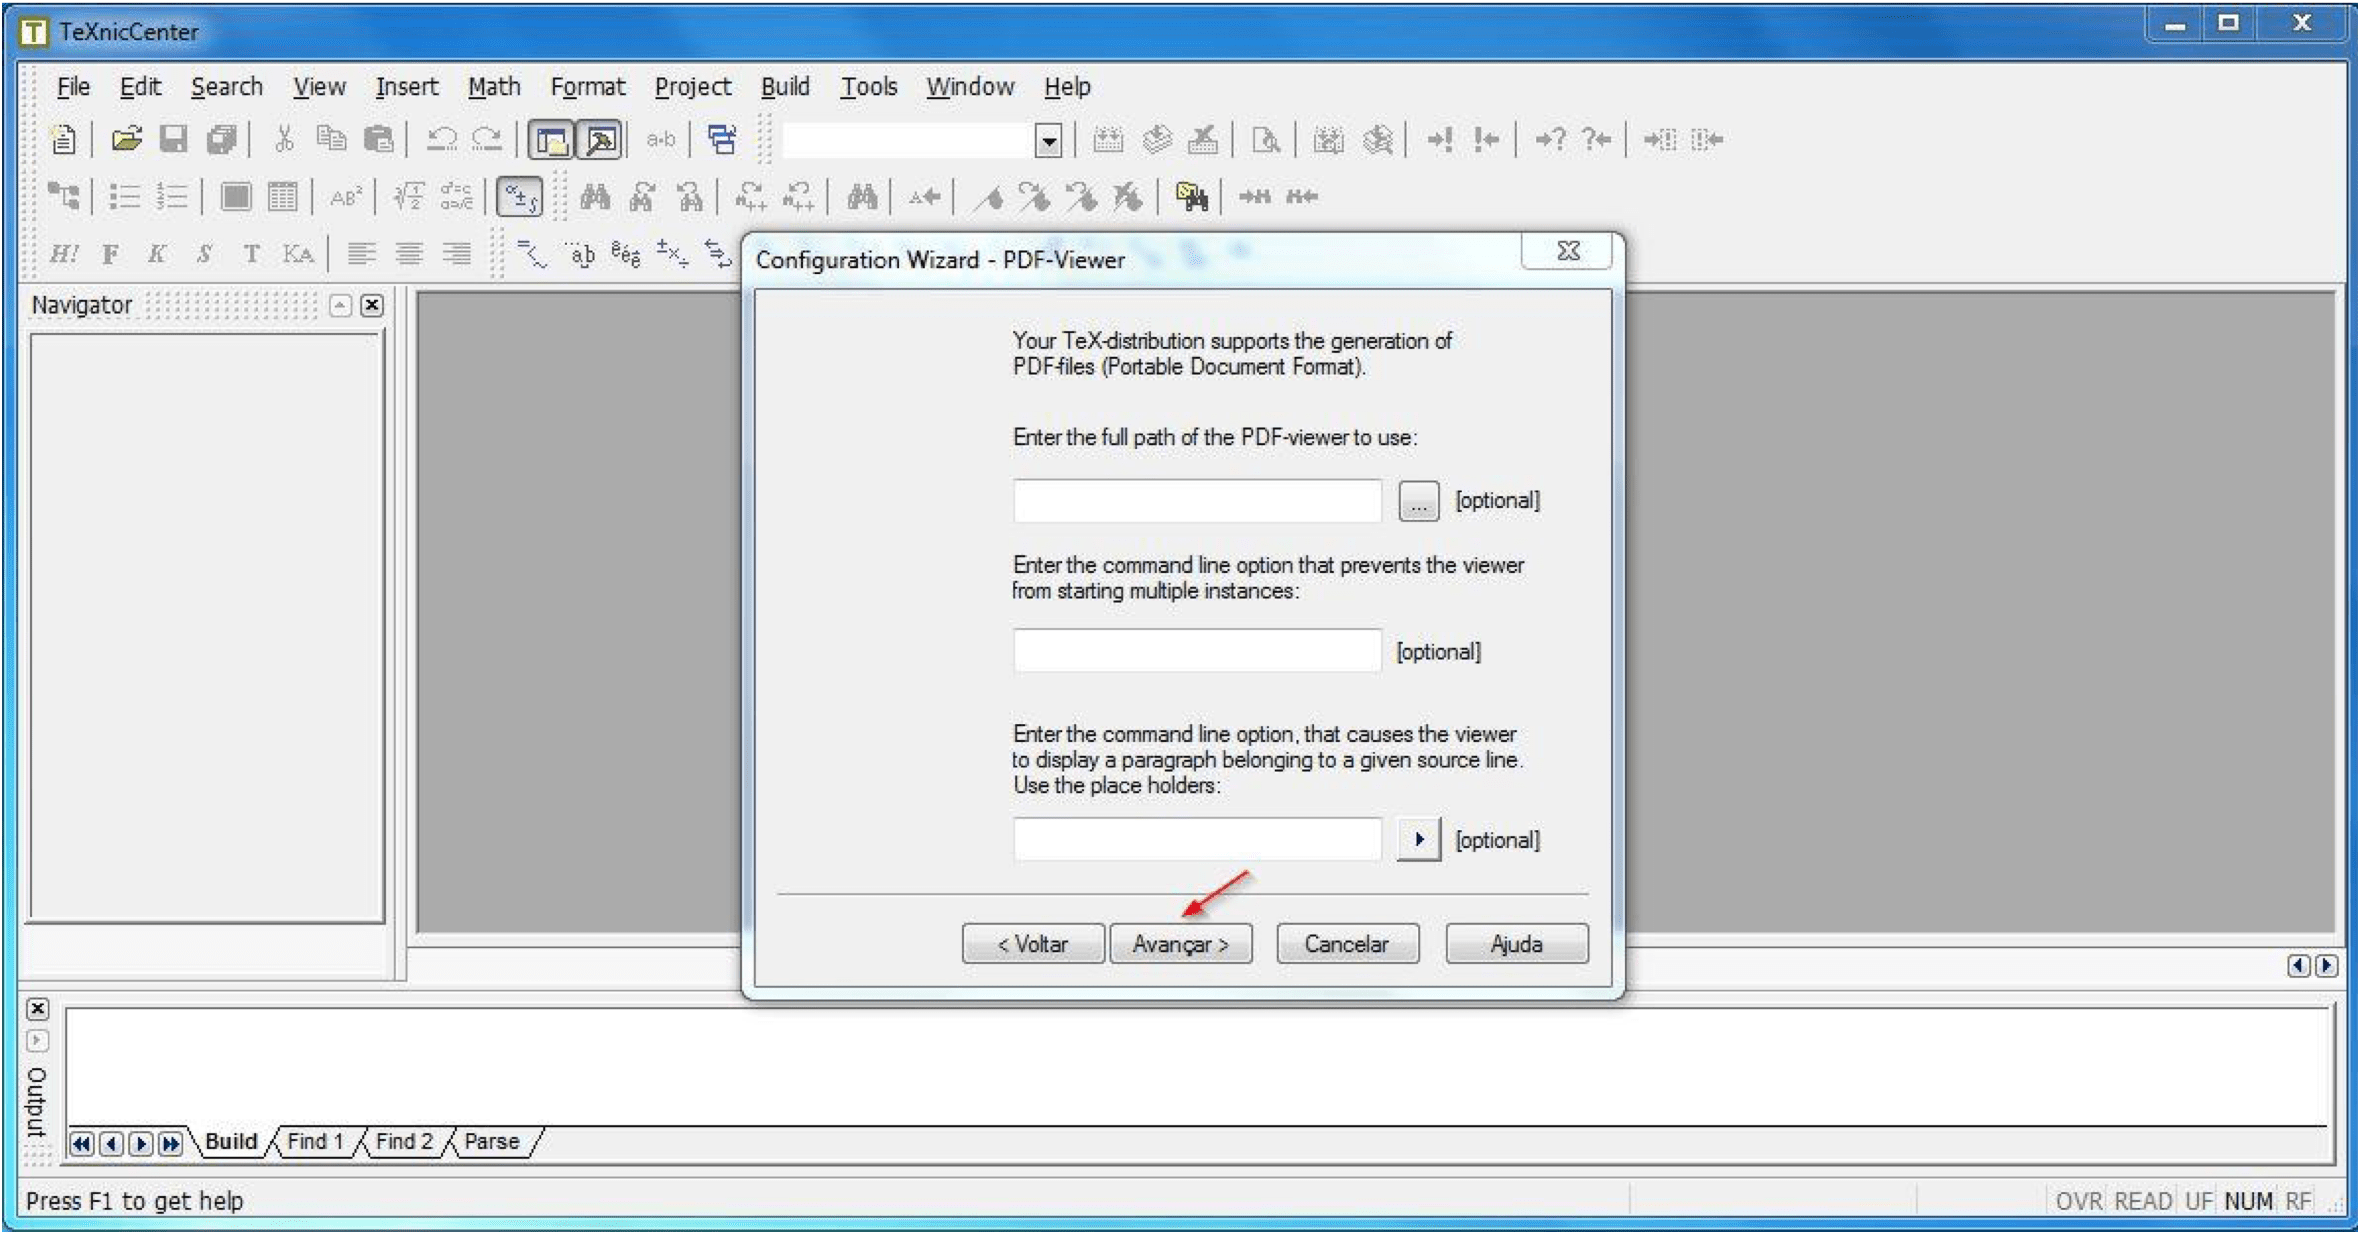
\includegraphics[width=1.0\textwidth]{./fig/texniccenter17}
  \caption{Configuração do TeXnicCenter - Sexta tela.}
  \fontefig{\cite{texnic}}
\end{figure}
\item Serão exibidos os nomes das configurações que serão feitas, apenas clique no botão \textbf{Concluir} para finalizar a configuração.
\begin{figure}[H]
  \centering
  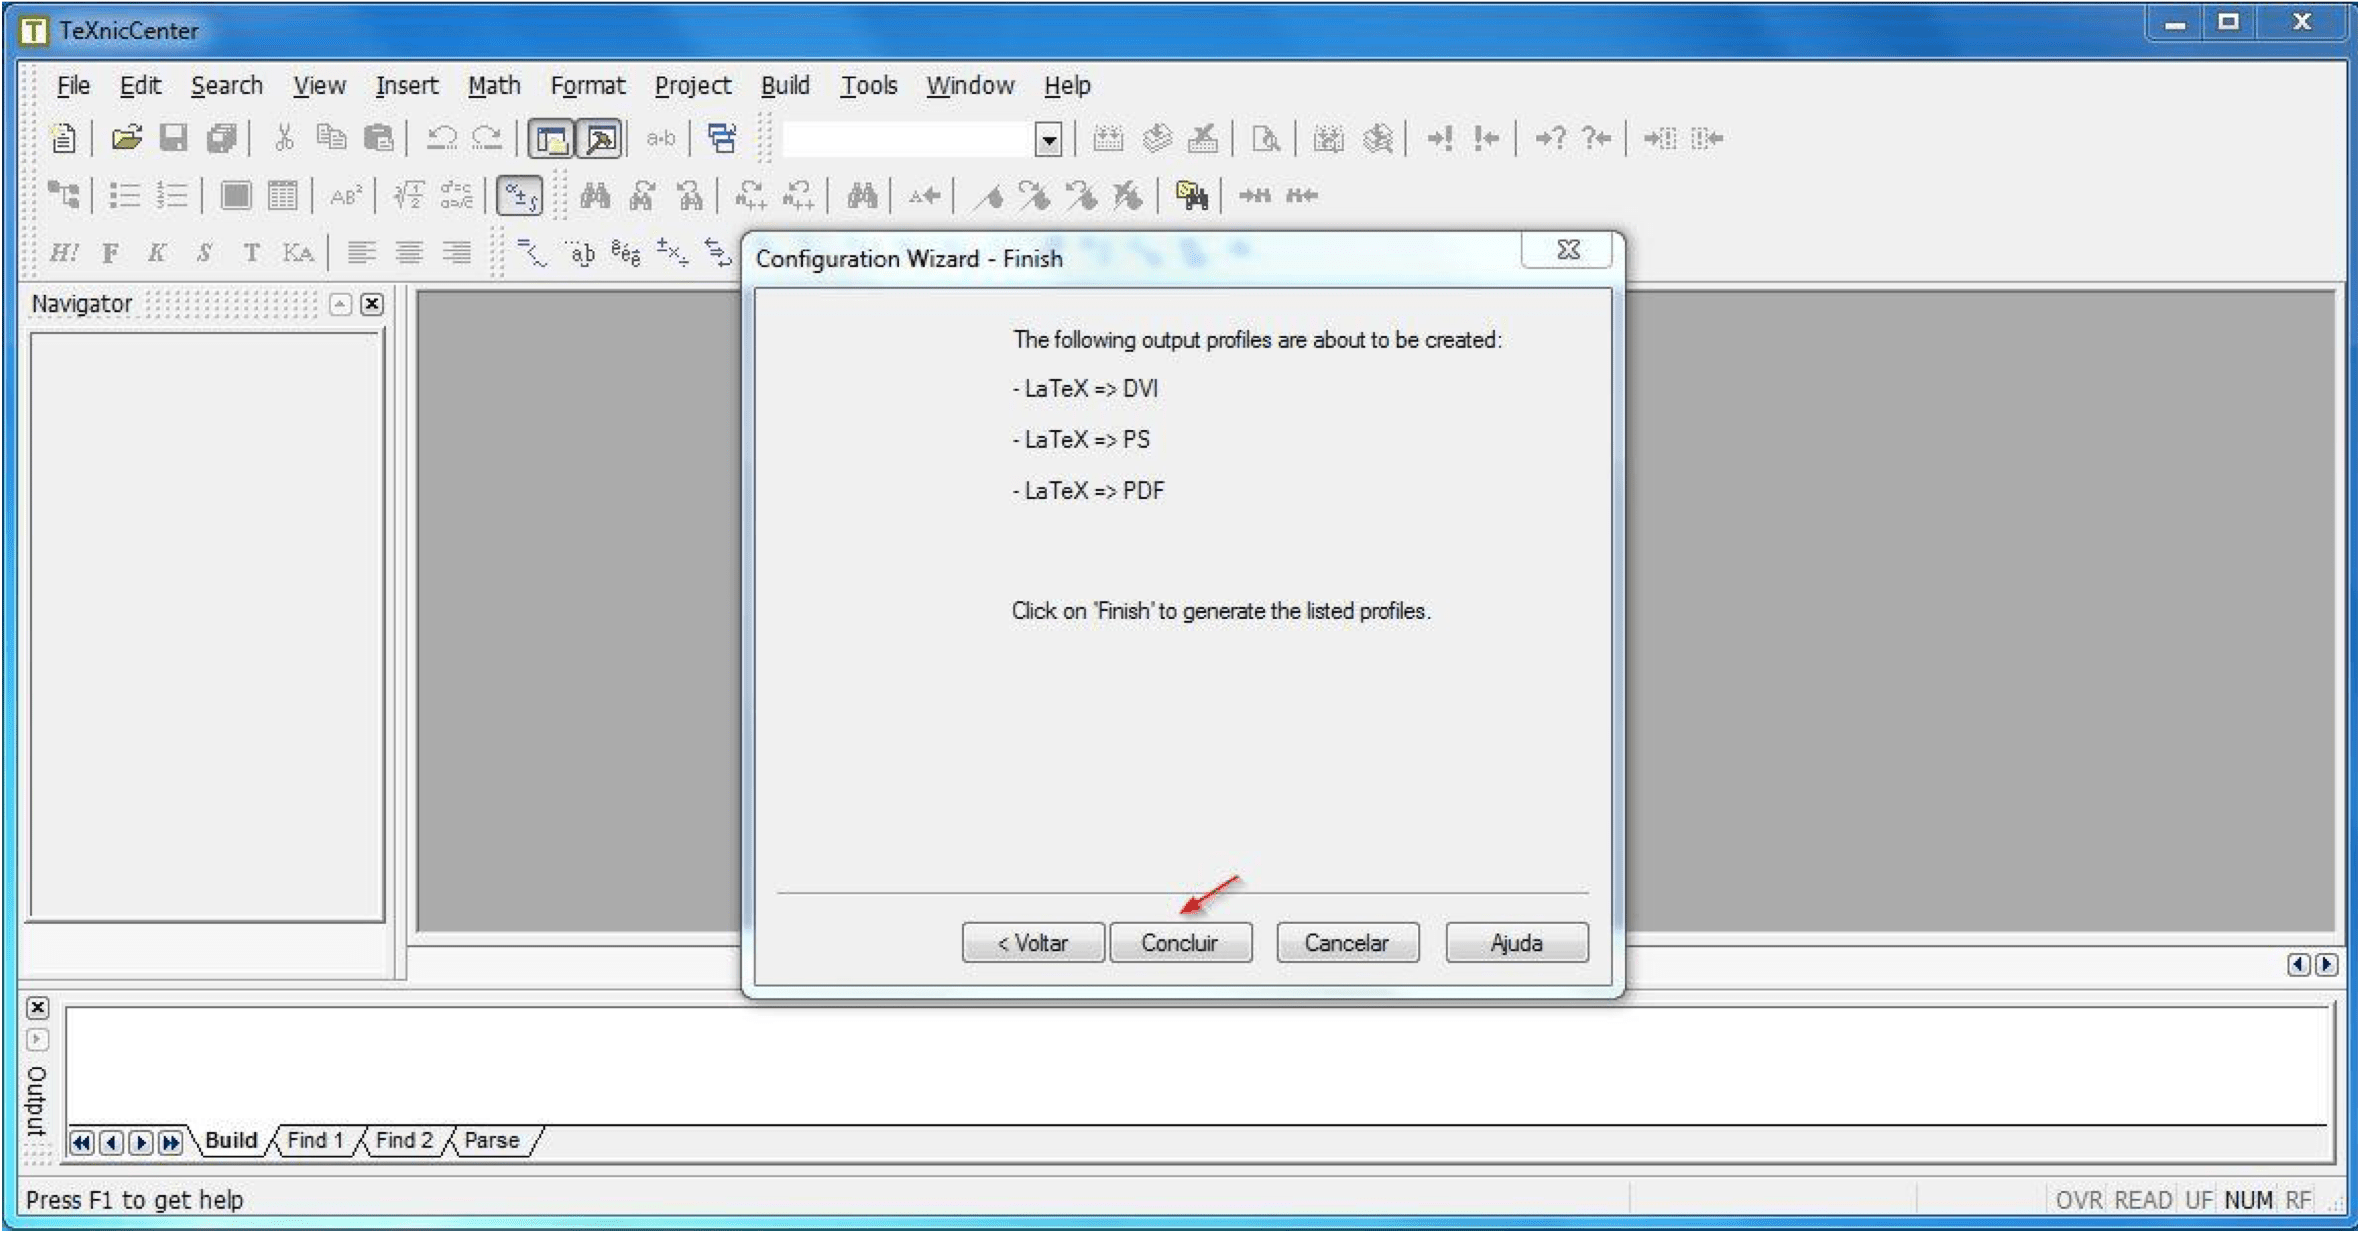
\includegraphics[width=1.0\textwidth]{./fig/texniccenter18}
  \caption{Configuração do TeXnicCenter - Sétima tela.}
  \fontefig{\cite{texnic}}
\end{figure}
\end{enumerate}

\section{Instalando o corretor ortográfico}

Por padrão o TeXnicCenter não vem com corretor ortográfico para português. Para instalá-lo siga os passos a seguir \cite{texnic}.

\begin{enumerate}
\item Faça o download do verificador ortográfico em \url{https://pt-br.libreoffice.org/projetos/vero/}.
\begin{figure}[H]
  \centering
  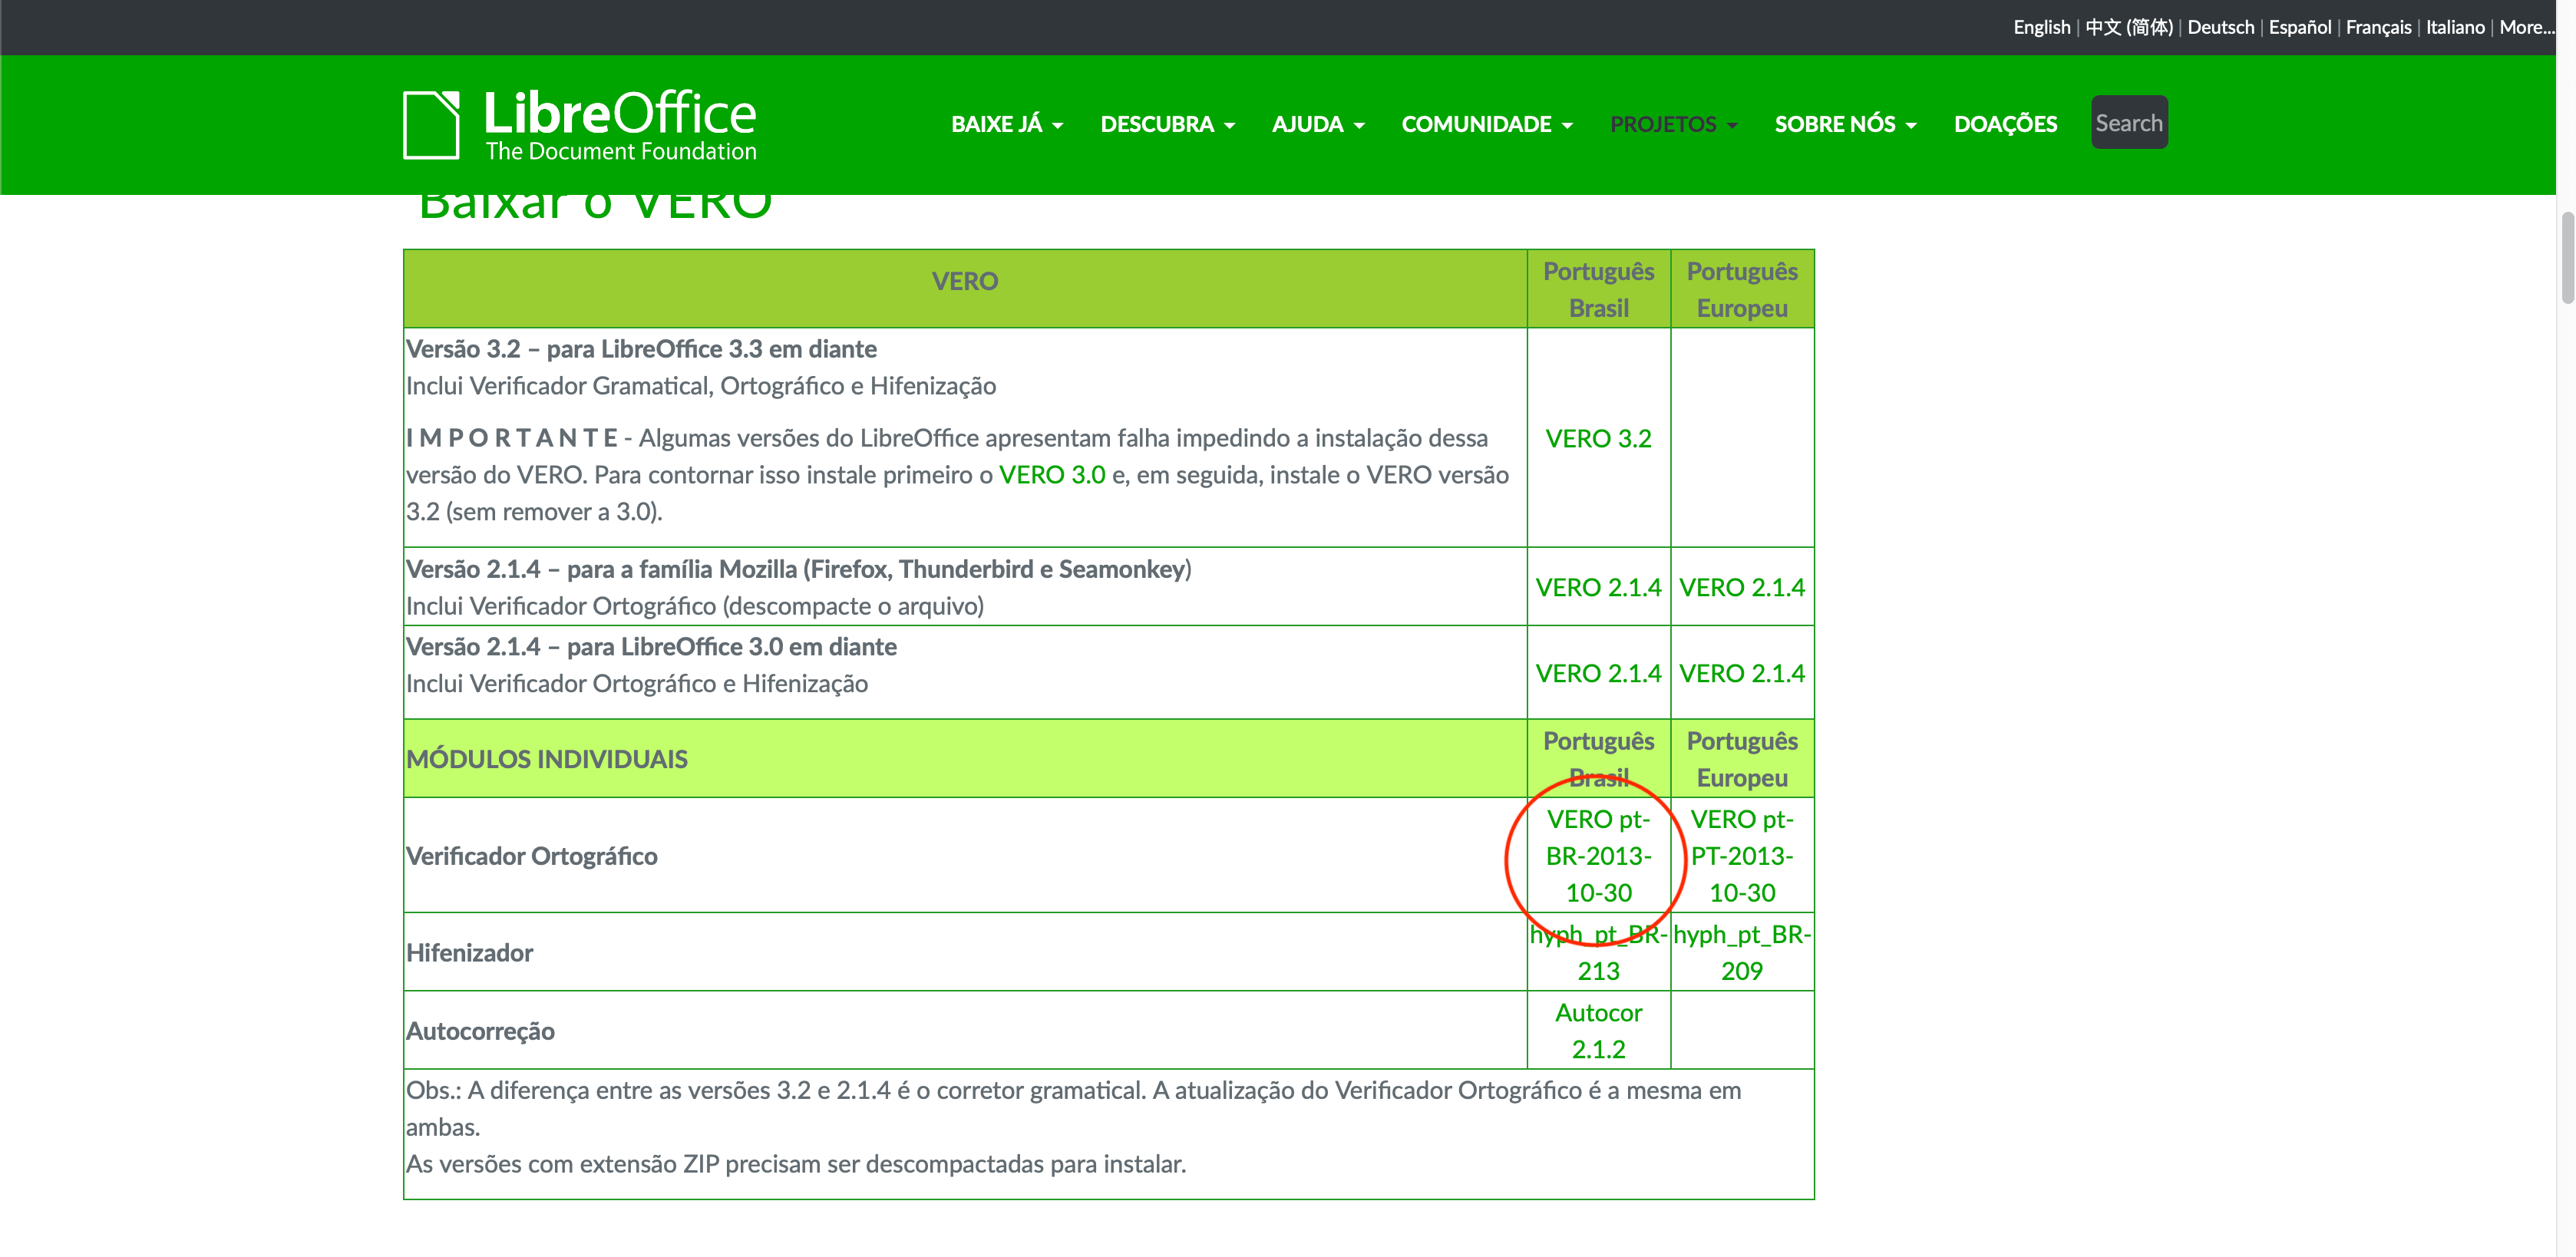
\includegraphics[width=1.0\textwidth]{./fig/vero01}
  \caption{Página de download do corretor ortográfico.}
  \fontefig{Elaborado pelo autor}
\end{figure}
\item Na pasta do arquivo descompactado anteriormente localize os arquivos \aspas{pt\_BR.aff} e \aspas{pt\_BR.dic} e copie eles.
\begin{figure}[H]
  \centering
  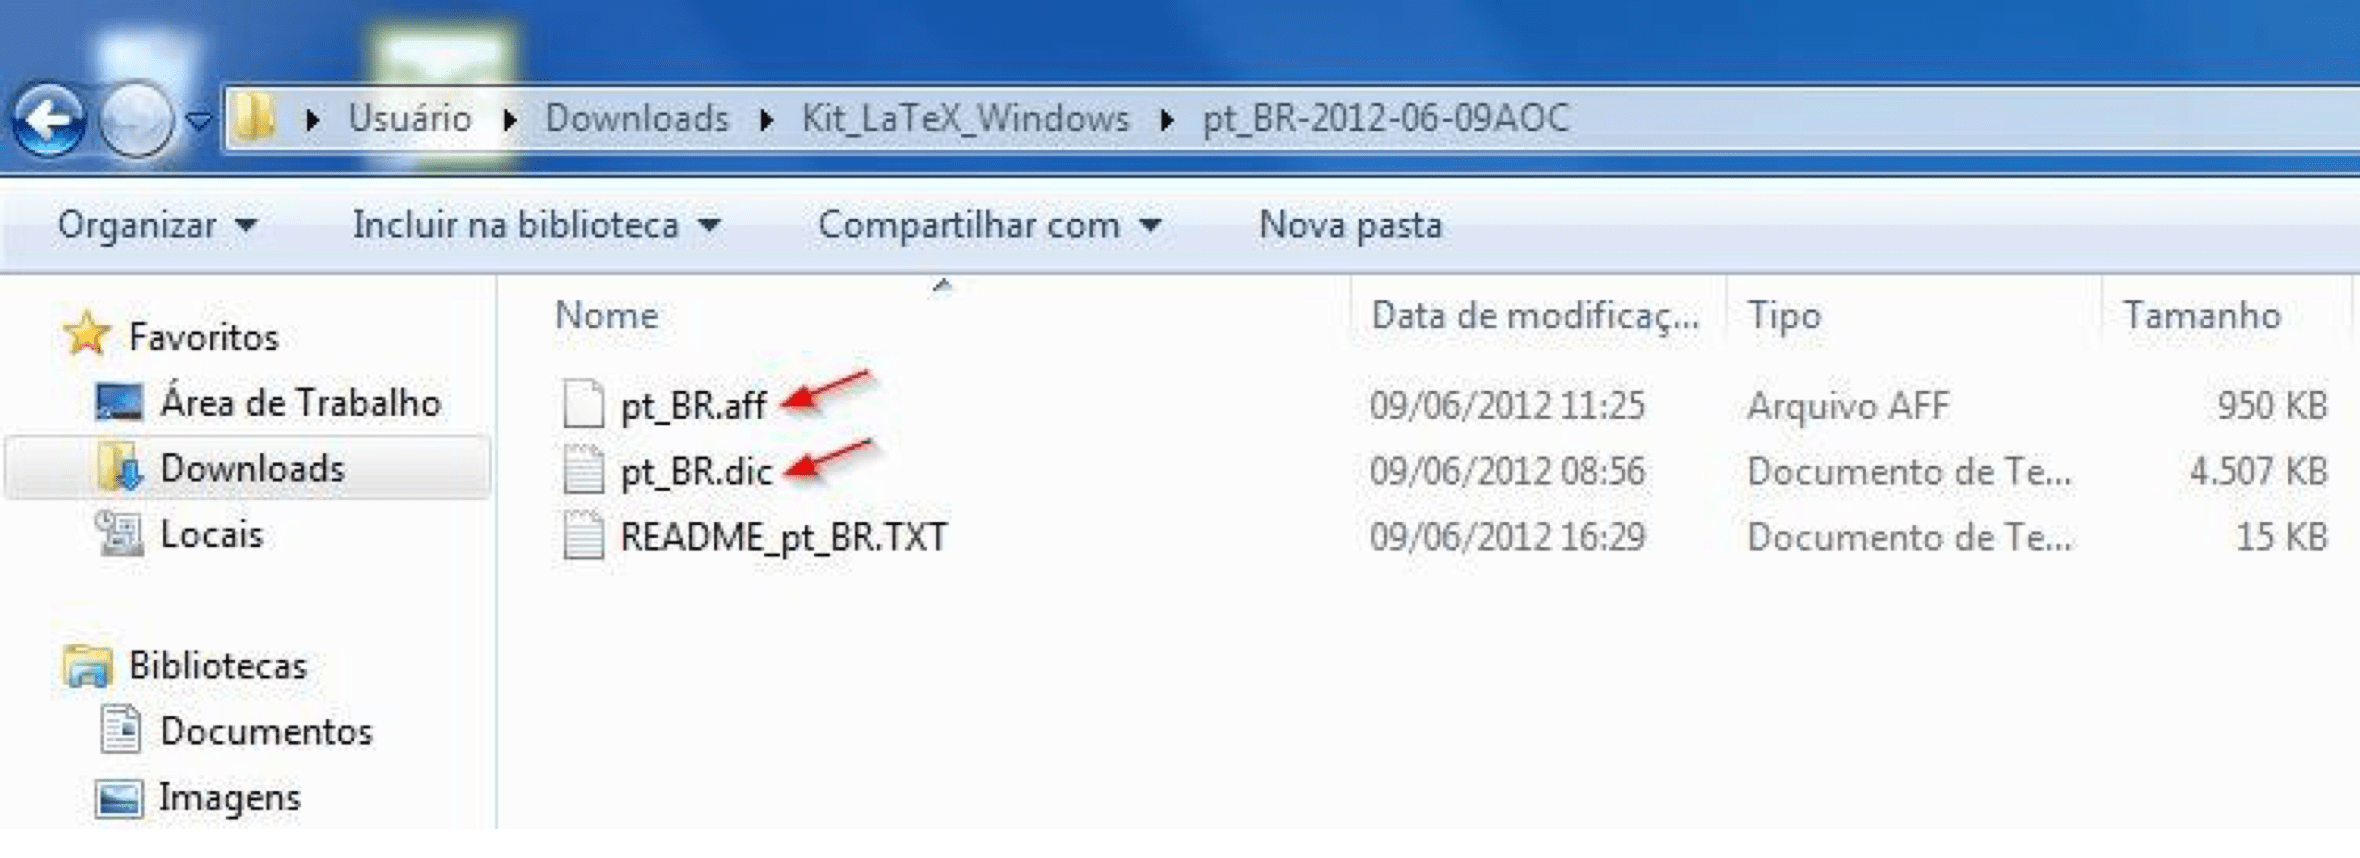
\includegraphics[width=1.0\textwidth]{./fig/vero02}
  \caption{Instalação do corretor ortográfico - Primeira tela.}
  \fontefig{\cite{texnic}}
\end{figure}
\item Localize a pasta de instalação do TeXnicCenter (neste tutorial é a pasta: \aspas{C:$\backslash$Program Files (x86)$\backslash$TeXnicCenter}, mas pode variar de acordo com a versão do Windows utilizada) e dentro dela localize a pasta \textbf{Language}.
\begin{figure}[H]
  \centering
  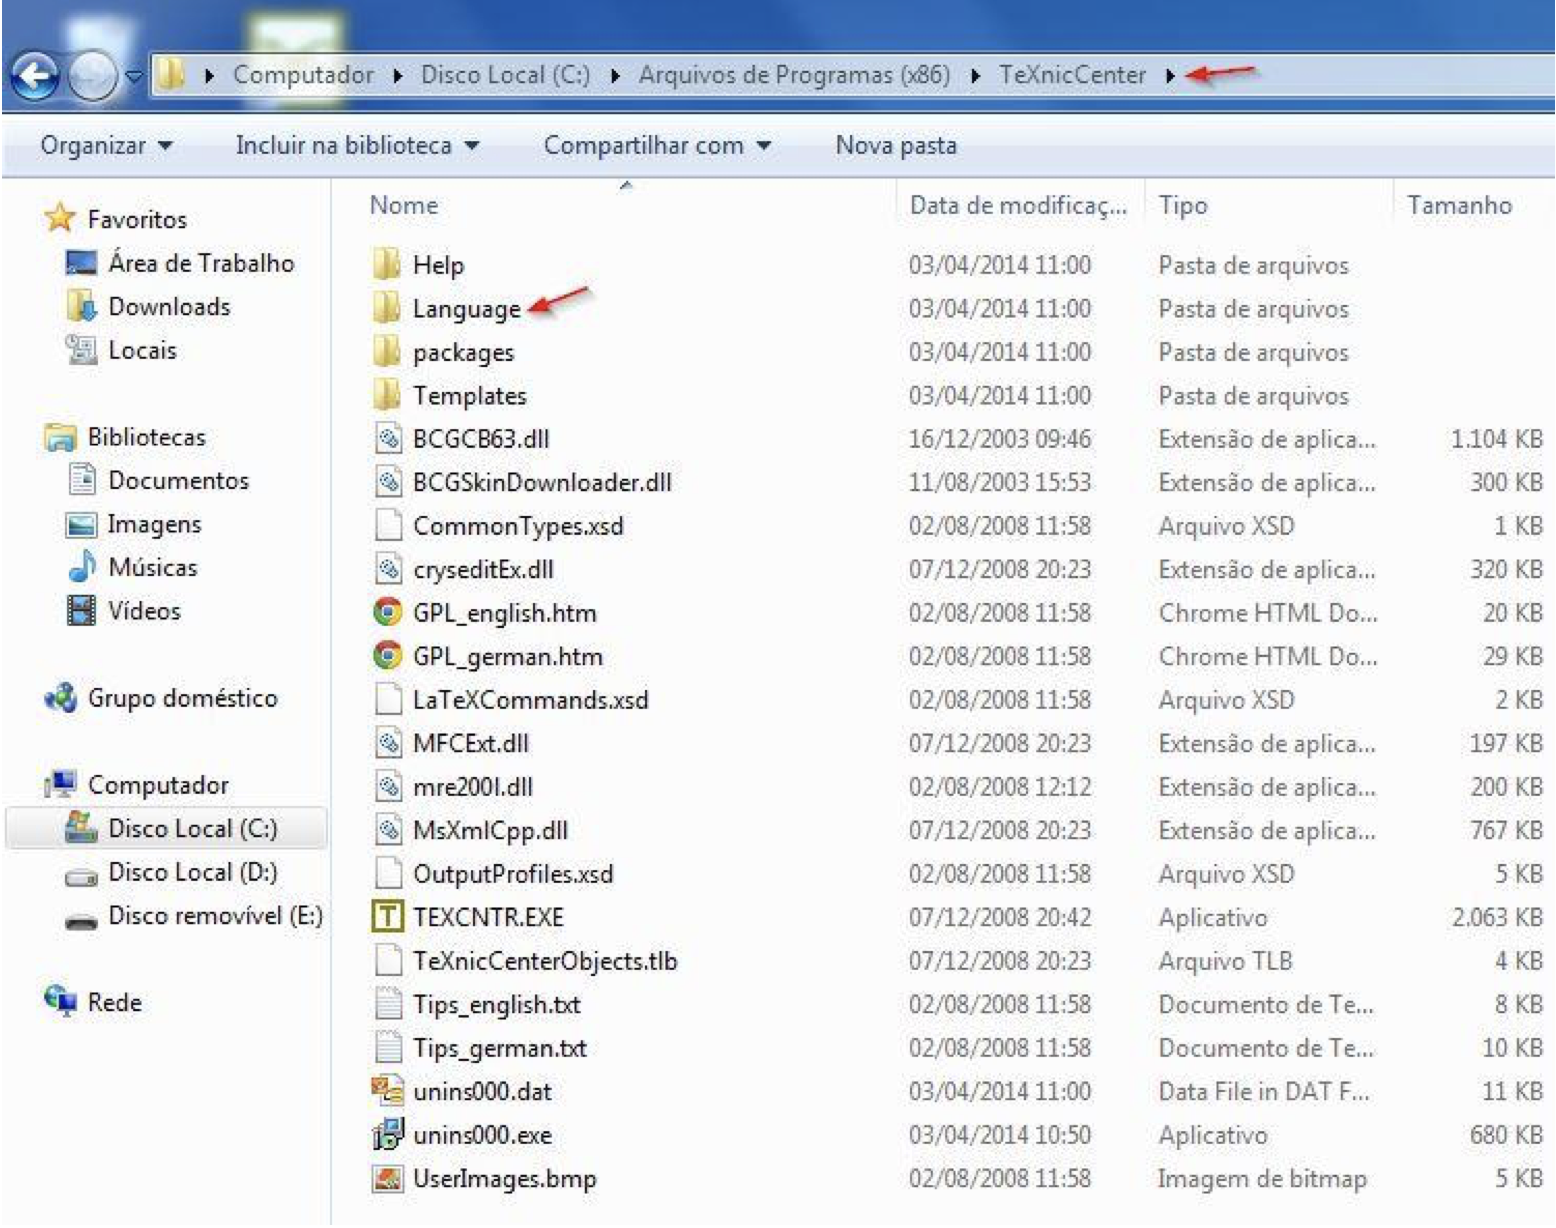
\includegraphics[width=1.0\textwidth]{./fig/vero03}
  \caption{Instalação do corretor ortográfico - Segunda tela.}
  \fontefig{\cite{texnic}}
\end{figure}
\item Cole os arquivos anteriormente copiados dentro da pasta \textbf{Language}.
\begin{figure}[H]
  \centering
  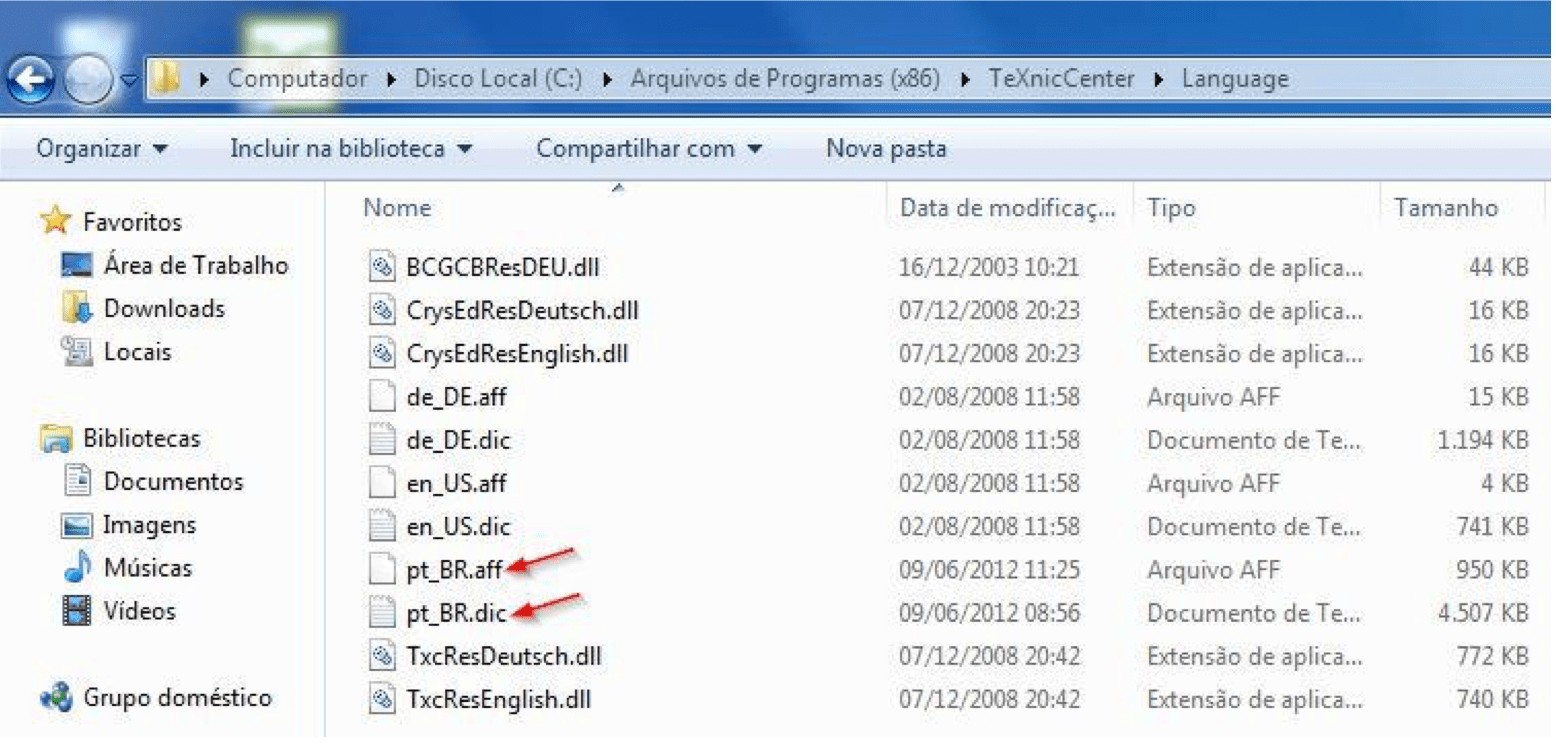
\includegraphics[width=1.0\textwidth]{./fig/vero04}
  \caption{Instalação do corretor ortográfico - Terceira tela.}
  \fontefig{\cite{texnic}}
\end{figure}
\item Para configurar o verificador ortográfico no TeXnicCenter, abra o aplicativo e no menu clique na opção \textbf{Tools}.
\begin{figure}[H]
  \centering
  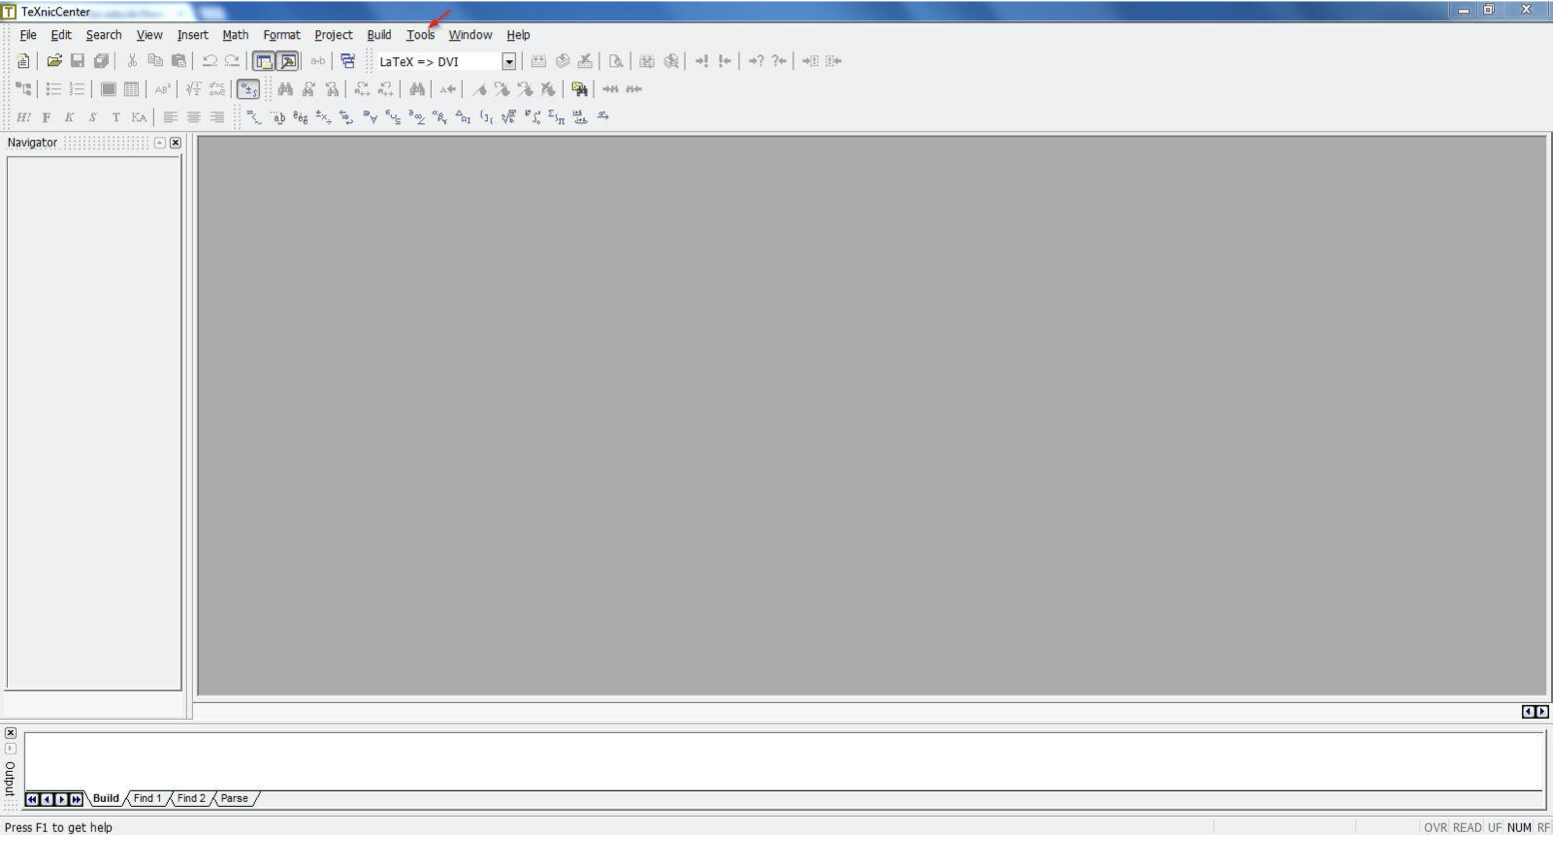
\includegraphics[width=1.0\textwidth]{./fig/vero05}
  \caption{Instalação do corretor ortográfico - Quarta tela.}
  \fontefig{\cite{texnic}}
\end{figure}
\item Agora nas opções abertas do menu é necessário clicar na opção \textbf{Options...}.
\begin{figure}[H]
  \centering
  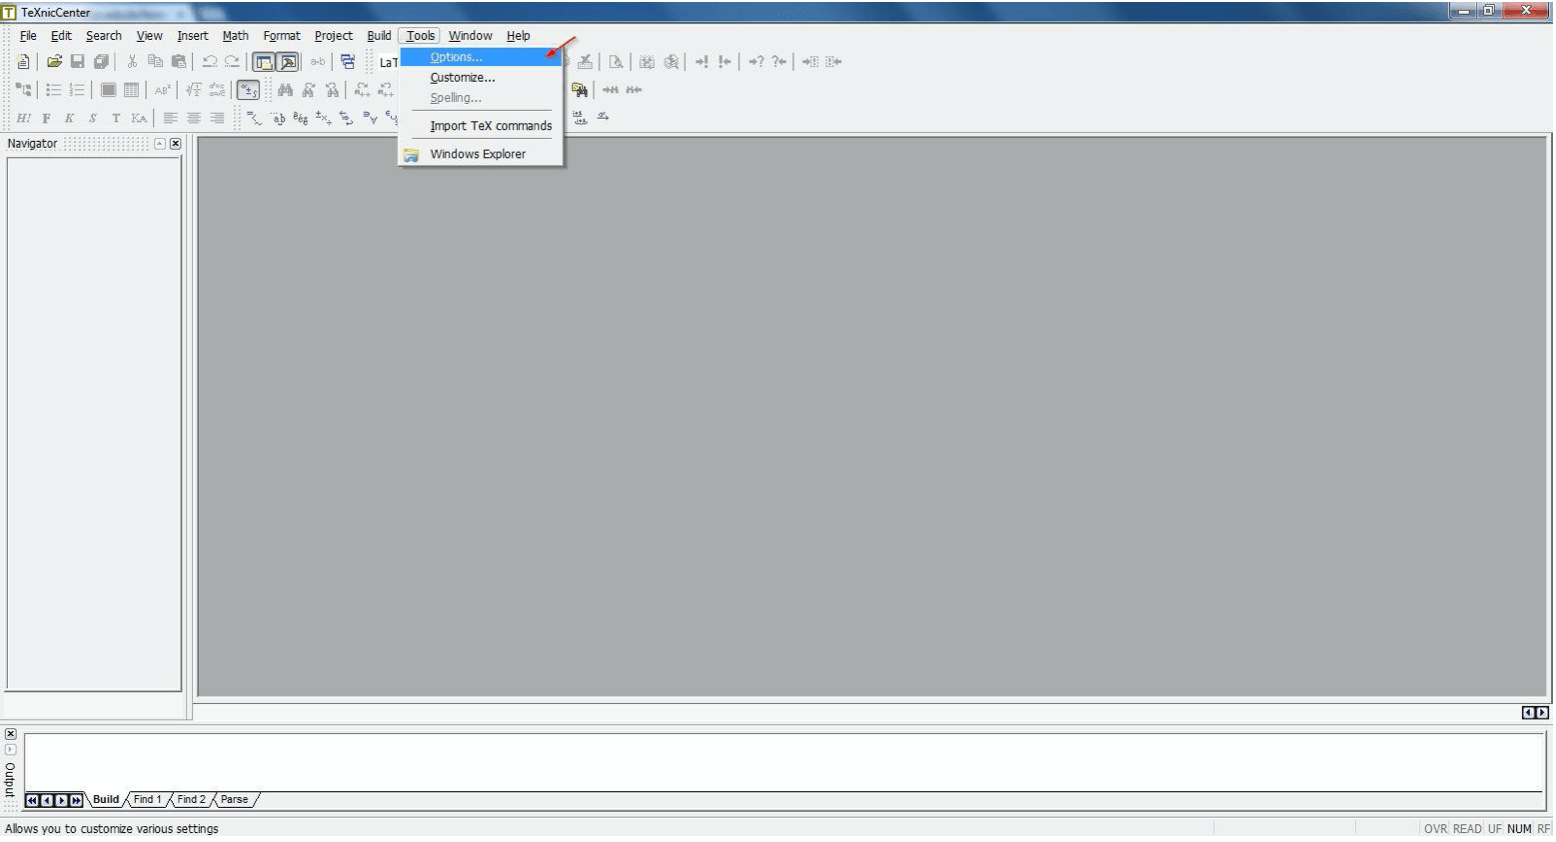
\includegraphics[width=1.0\textwidth]{./fig/vero06}
  \caption{Instalação do corretor ortográfico - Quinta tela.}
  \fontefig{\cite{texnic}}
\end{figure}
\item Na janela de opções aberta clique na aba \textbf{Spelling}.
\begin{figure}[H]
  \centering
  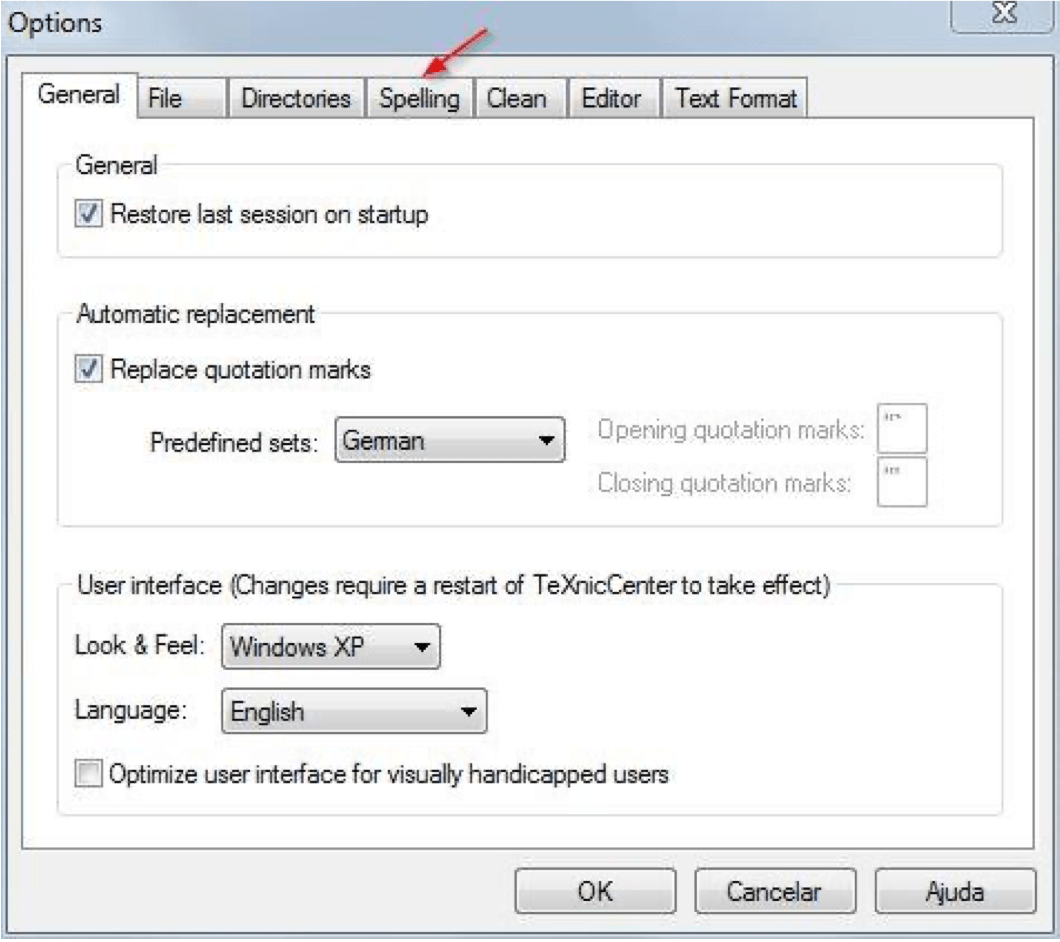
\includegraphics[width=0.6\textwidth]{./fig/vero07}
  \caption{Instalação do corretor ortográfico - Sexta tela.}
  \fontefig{\cite{texnic}}
\end{figure}
\item Na Na aba aberta na opção \textbf{Language} selecione \textbf{pt}, na opção \textbf{Dialect} selecione \textbf{BR}, na opção \textbf{Locale} selecione \textbf{Portuguese\_Brazil.1252} e na seção \textbf{Options} clique na caixa ao lado de \textbf{Check spelling while typing} para setar as opções de correção ortográfica. Após selecionadas as opções clique no botão \textbf{OK}.
\begin{figure}[H]
  \centering
  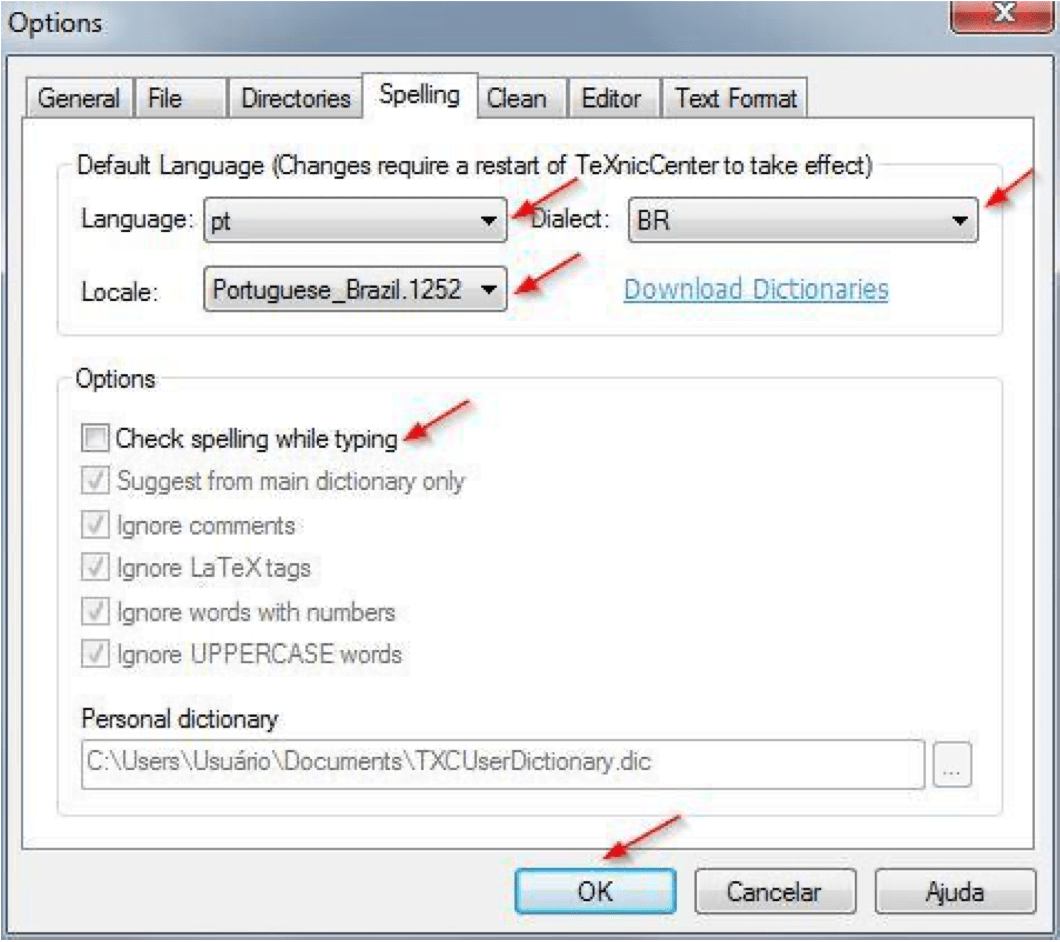
\includegraphics[width=0.6\textwidth]{./fig/vero08}
  \caption{Instalação do corretor ortográfico - Sétima tela.}
  \fontefig{\cite{texnic}}
\end{figure}
\item A caixa de diálogo abaixo será exibida informando que é necessário reiniciar o TeXnicCenter para que as opções selecionadas anteriormente tenham efeito. Clique no botão \textbf{OK} para fechar.
\begin{figure}[H]
  \centering
  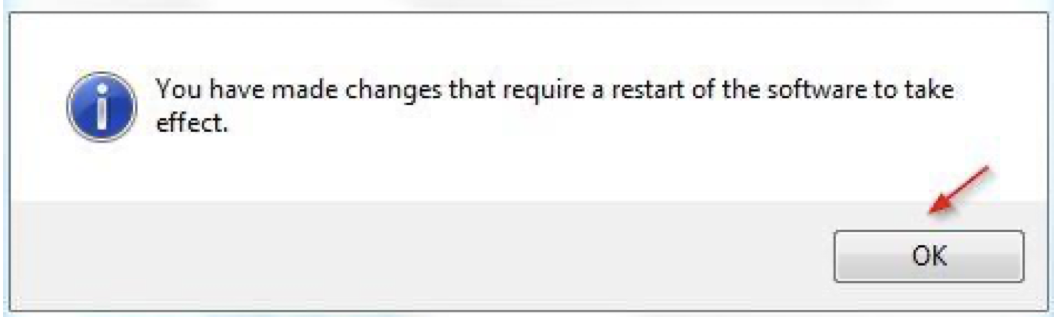
\includegraphics[width=0.6\textwidth]{./fig/vero09}
  \caption{Instalação do corretor ortográfico - Oitava tela.}
  \fontefig{\cite{texnic}}
\end{figure}
\item Será exibida uma caixa de diálogo informando que o dicionário de usuário não foi encontrado e que foi criado um novo dicionário pessoal vazio. Clique no botão \textbf{OK} para fechar.
\begin{figure}[H]
  \centering
  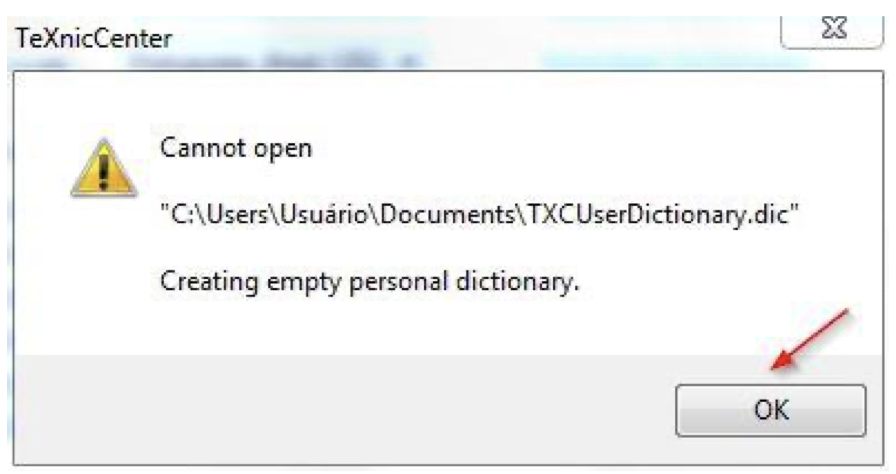
\includegraphics[width=0.5\textwidth]{./fig/vero10}
  \caption{Instalação do corretor ortográfico - Nona tela.}
  \fontefig{\cite{texnic}}
\end{figure}
\end{enumerate}

\section{Usando o \LaTeX\ online}

Em vez de utilizar o \LaTeX\ localmente em seu computador você pode utilizá-lo online usando o Overleaf, uma plataforma de escrita colaborativa, cujo objetivo principal  é facilitar o o processo de escrita acadêmica.

Inicialmente crie uma conta em \url{https://www.overleaf.com}. Depois, acesse o endereço \url{https://overleaf.com/docs?snip_uri=https://github.com/raphaeldeaquino/classe-ifg/archive/main.zip} que o projeto será criado automaticamente.
\chapter{Descrição da \textsf{classe-ifg}}
\label{cap:descr}

%% - - - - - - - - - - - - - - - - - - - - - - - - - - - - - - - - - - -
\section{Opções da classe}
\label{sec:opcoes}
Para usar esta classe num documento \LaTeXe, coloque a pasta \verb|formatacao| numa pasta onde o compilador \LaTeX\ pode achá--lo (normalmente na mesma pasta que seu arquivo \verb|.tex|), e defina--o como o estilo do seu documento. Por exemplo, uma dissertação de mestrado:
\begin{verbatim}
\documentclass[dissertacao]{classe-ifg}
...
\begin{document}
\end{verbatim}

As opções da classe são \verb|[dissertacao]| (para dissertação de mestrado), \verb|[qualificacaom]| (para qualificação de mestrado) e \verb|[monografia]| (para monografia final de especialização). Se nenhuma opção for declarada, o documento é considerado como uma dissertação de mestrado. %Com a opção \verb|[nocolorlinks]| todos os {\em links} de navegação no texto ficam na cor preta. O ideal é usar esta opção para gerar o arquivo para impressão, pois a qualidade da impressão dos {\em links} fica superior.


%% - - - - - - - - - - - - - - - - - - - - - - - - - - - - - - - - - - -
\section{Parâmetros da classe}
\label{sec:param}
Os elementos pré-textuais são definidos página por página e dependem da correta definição dos parâmetros listados a seguir (os elementos que não foram aplicáveis como, por exemplo, \verb|\orientadora| quando orientador é do sexo masculino, devem permanecer comentados usando \% no início da respectiva linha):

% \setlength{\topsep}{5.2em}
 \begin{itemize}%\addtolength{\itemsep}{-0.7em}
\item \verb|\autor| : Nome completo do autor, começando pelo primeiro nome (ex.: José da Silva);
\item \verb|\autorR| : Nome completo do autor, começando pelo último sobrenome (ex.: da Silva, José);
\item \verb|\sautor| : Nome completo do segundo autor (quando aplicável), começando pelo primeiro nome (ex.: José da Silva);
\item \verb|\sautorR| : Nome completo do segundo autor (quando aplicável), começando pelo último sobrenome (ex.: da Silva, José);
\item \verb|\titulo| : Título da dissertação ou monografia de conclusão de curso;
\item \verb|\subtitulo| : Se tiver um subtítulo, use este macro para defini--lo;

\item \verb|\cidade| : A cidade de edição. 
\item \verb|\dia| : Dia do mês da data de defesa (01--31);
\item \verb|\mes| : Mês da data de defesa (01--12);
\item \verb|\ano| : Ano da data de defesa;

\item \verb|\orientador| : Nome completo do orientador, começando pelo primeiro nome;
\item \verb|\orientadorR| : Nome completo do orientador, começando pelo último sobrenome;

\item \verb|\orientadora| : Nome completo da orientadora, começando pelo primeiro nome; use este comando e o próximo se for orientadora e não orientador.
\item \verb|\orientadoraR| : Nome completo do orientadora, começando pelo último sobrenome;

\item \verb|\coorientador| : Nome completo do co--orientador, começando pelo primeiro nome;
\item \verb|\coorientadorR| : Nome completo do co--orientador, começando pelo último sobrenome;

\item \verb|\coorientadora| : Nome completo da coorientadora, começando pelo primeiro nome; use este comando e o próximo se for coorientadora e não coorientador.
\item \verb|\coorientadoraR| : Nome completo do coorientadora, começando pelo último sobrenome;

\item \verb|\universidadeco| : Nome da universidade do coorientador;
\item \verb|\unico| : Sigla da universidade do coorientador;
\item \verb|\unidadeco| : Nome da unidade acadêmica do coorientador.\footnote{Se não tiver um co--orientador, não defina esses últimos sete parâmetros.}
\end{itemize}

%% - - - - - - - - - - - - - - - - - - - - - - - - - - - - - - - - - - -
\section{Elementos Pré--Textuais}
\label{sec:pre}
Os elementos pré--textuais são definidos página por página, conforme descritos a seguir:

\paragraph{capa\\}
\verb|\capa| : Gera o modelo da capa externa do trabalho. Esta página servirá apenas como modelo para a encadernação da versão final do texto. Nenhum dado é necessário.

\paragraph{rosto\\}
\verb|\rosto| : Gera a folha de rosto, a qual é a primeira folha interna do trabalho. Nenhum dado é necessário.

\paragraph{ficha\\}
\verb|\ficha| : Inclui a ficha catalográfica que deve constar como um arquivo PDF cujo nome deve necessariamente ser \verb|ficha.pdf|. Este arquivo deve estar localizado na mesma pasta que seu arquivo \verb|.tex|. Comente este comando até ter a versão final da dissertação.

\paragraph{aprovacao\\}
\verb|\input{./pre/preAprovacao}| : Entrada para o nome dos examinadores, exceto o(s) orientador(es). Edite o arquivo equivalente com os parâmetros nele descritos.

%\paragraph{curriculo\\}
%\verb|\aprovacao| : ambiente para a reprodução do termo de aprovação da Banca Examinadora da tese ou dissertação.
%

\paragraph{dedicatória\\}
\verb|\input{./pre/preDedicatoria| : ambiente para escrever a dedicatória. É possível trocar o espaçamento dentro desse ambiente do mesmo jeito que no \LaTeX\ padrão.

\paragraph{agradecimentos\\}
\verb|\begin{agradecimentos}

Texto de agradecimento.

\end{agradecimentos}| : ambiente para escrever os agradecimentos. É possível trocar o espaçamento dentro desse ambiente do mesmo jeito que no \LaTeX\ padrão.

\paragraph{resumo\\}
\verb|\chaves{palavra 1, palavra 2, palavra 3} % Palavras chave separadas por vírgula

\begin{resumo}

De 150 a 500 palavras - trabalhos acadêmicos (teses, dissertações e outros) e relatórios técnico-científicos (ABNT NBR 6028)

\end{resumo}
| : A lista das palavras chaves, separadas por `;'. Deve ser definido antes do ambiente \verb|\resumo|, o qual é usado para escrever o resumo em português.

\paragraph{abstract\\}
\verb|\keys| : A lista das palavras chaves em inglês, separadas por `;'. Deve ser definido antes do ambiente \verb|\abstract|, o qual contém 1 argumento e é usado escrever o resumo em inglês. O argumento deve ser o título do trabalho em inglês.

\paragraph{tabelas\\}
\verb|\tabelas| : Macro com 1 argumento opcional para gerar as tabelas. O argumento pode ser:
\begin{itemize}
 \item nada [] : gera apenas o sumário;
 \item \textsf{fig} : gera o sumário e uma lista de figuras;
 \item \textsf{tab} : gera o sumário e uma lista de tabelas;
 \item \textsf{alg} : gera o sumário e uma lista de algoritmos;
 \item \textsf{cod} : gera o sumário e uma lista de programas.
 \item \textsf{figtab} : gera o sumário, uma lista de tabelas, e uma lista de figuras;
 \item \textsf{figtabalg} : gera o sumário e listas de tabelas, de figuras e de algoritmos;
 \item \textsf{figtabalgcod} : gera o sumário e listas de tabelas, de figuras, de algoritmos e de programas;
 \item (qualquer outra coisa) : gera somente o sumário.
\end{itemize}

Pode-se usar qualquer combinação dessas opções. Por exemplo:
\begin{itemize}
 \item \textsf{figtab} : gera o sumário e listas de figuras e tabelas,
 \item \textsf{figtabcod} : gera o sumário e listas de figuras, tabelas e códigos de programas;
 \item \textsf{figtabalg} : gera o sumário e listas de figuras, tabelas e algoritmos;
 \item \textsf{figtabalgcod} : gera o sumário e listas de figuras, tabelas, algoritmos e códigos de programas
\end{itemize}

\paragraph{epígrafe\\}
\verb|\epigrafe| : Macro com 3 argumentos que permite editar um epígrafe. O primeiro argumento é o texto da citação. O segundo argumento é o nome do autor da citação. O terceiro argumento é o título da referência à qual a citação pertence.

\chapter{Elementos do texto}
\label{cap:texto}

Neste capítulo é dada uma visão geral sobre os elementos que podem ser utilizados no texto e código de inserção em \LaTeX.

% - - - - - - - - - - - - - - - - - - - - - - - - - - - - - - - - - - -
\section{Seccionamento de Documentos}
\label{sec:sec} 

O \LaTeX pode organizar, numerar e indexar capítulos e seções do documento. Existem até 7 níveis de profundidade para definir seções, dependendo da classe do documento:

\begin{quadro}[!ht]
\caption{Níveis de seccionamento de documentos em \LaTeX.}
\label{qua:niveis}
\begin{center}
\begin{tabular}{|c|c|}        
\hline
\textbf{Nível} & \textbf{Comando}\\ \hline\hline
-1 & \verb|\part| \\
\hline
0 & \verb|\chaper| \\
\hline
1 & \verb|\section| \\
\hline
2 & \verb|\subsection| \\
\hline
3 & \verb|\subsubsection| \\
\hline
4 & \verb|\paragraph| \\
\hline
5 & \verb|\subparagraph| \\
\hline
\end{tabular}
\end{center}
\fontequa{Elaborado pelo autor}
\end{quadro}

Para documentos com a \texttt{classe-ifg} utilize somente a partir do nível 0. Como exemplo, o código abaixo insere um capítulo que possui uma seção com uma subseção:

\begin{verbatim}
\chapter{Título do capítulo}
\label{cap:id}

Texto inicial do capítulo ...

\section{Título da seção}
\label{cap:sec}

Texto inicial da seção ...

\subsection{Título do subseção}
\label{cap:subsec}

Texto da subseção ...
\end{verbatim}

O comando \verb|\label| define um rótulo para fazer referência ao elemento rotulado. Como exemplo, este capítulo foi rotulado usando \verb|\label{cap:texto}|, de forma que o código \verb|Capítulo \ref{cap:texto}| produz Capítulo \ref{cap:texto}.

% - - - - - - - - - - - - - - - - - - - - - - - - - - - - - - - - - - -
\section{Listas}
\label{sec:listas} 

As listas são criadas definindo o tipo de lista e os itens que as formam, conforme descrito a seguir.

\subsection{Listas não ordenadas}

As listas não ordenadas (não numeradas) são produzidas pelo ambiente \verb|itemize|. Cada entrada deve ser precedida pelo comando \verb|\item|. A seguir está o código de uma lista não ordenada e o resultado produzido.

Código:

\begin{verbatim}
\begin{itemize}
    \item As entradas individuais são indicadas com um ponto preto, o 
denominado marcador.
    \item O texto nas entradas pode ter qualquer comprimento.
\end{itemize}
\end{verbatim}

Resultado:

\begin{itemize}
	\item As entradas individuais são indicadas com um ponto preto, o denominado marcador.
	\item O texto nas entradas pode ter qualquer comprimento.
\end{itemize}

\subsection{Listas ordenadas}

As listas ordenadas são geradas por um ambiente \verb|enumerate| e cada entrada deve ser precedida pelo comando \verb|\item|, que irá gerar automaticamente o número que rotula o item. Os rótulos enumerados consistem em números sequenciais; esses números começam em 1 com cada chamada para o ambiente enumerado.

Código:

\begin{verbatim}
\begin{enumerate}
    \item Os rótulos consistem em números sequenciais.
    \item Os números começam em 1 com cada chamada para o ambiente 
enumerado.
\end{enumerate}
\end{verbatim}

Resultado:

\begin{enumerate}
    \item Os rótulos consistem em números sequenciais.
    \item Os números começam em 1 com cada chamada para o ambiente enumerado.
\end{enumerate}

\subsection{Listas Aninhadas}

Em \LaTeX\ é possível inserir uma lista dentro de outra lista. As listas acima podem ser incluídas umas nas outras, misturadas ou de um tipo, em uma profundidade de quatro níveis.

Código:

\begin{verbatim}
\begin{enumerate}
    \item Os rótulos consistem em números sequenciais.
    \begin{itemize}
        \item As entradas individuais são indicadas com um ponto preto, 
o denominado marcador.
        \item O texto nas entradas pode ter qualquer comprimento.
    \end{itemize}
    \item Os números começam em 1 com cada chamada para o ambiente 
enumerado.
\end{enumerate}
\end{verbatim}

Resultado:

\begin{enumerate}
    \item Os rótulos consistem em números sequenciais.
    \begin{itemize}
      \item As entradas individuais são indicadas com um ponto preto, o denominado marcador.
      \item O texto nas entradas pode ter qualquer comprimento.
    \end{itemize}
    \item Os números começam em 1 com cada chamada para o ambiente enumerado.
\end{enumerate}

% - - - - - - - - - - - - - - - - - - - - - - - - - - - - - - - - - - -
\section{Figuras}
\label{sec:figs} 
Rótulos de figuras e tabelas devem ser centralizados se tiverem até uma linha (Figura~\ref{fig:exemploFig1}), caso contrário devem estar justificados e identados em ambas as margens, como mostrado na Figura ~\ref{fig:exemploFig2}. Essa formatação já é realizada automaticamente pela \textsf{classe-ifg}.

Os compiladores \LaTeX\ provêem um mecanismo bastante simples para inclusão de figuras, o que pode ser feito com o auxílio de várias classes auxiliares (as mais comuns são \verb|graphic| e \verb|graphicx|). A \textsf{classe-ifg} usa o comando \verb|\includegraphics|, da classe \verb|graphicx|, para a inclusão de figuras e não é necessário você colocar a extensão do arquivo neste comando. Por exemplo, para a figura \ref{fig:exemploFig1} os comandos usados foram:

\begin{verbatim}
\begin{figure}[ht!]
  \centering
  
\includegraphics[width=0.4\textwidth]{fig/logo-ifg-vertical-goiania}
  \caption{Logo IFG.}
  \label{fig:exemploFig1}
 \end{figure}
 \fontefig{\cite{ifg2020}}
\end{verbatim}

O código \verb|[ht!]| após \verb|\begin{figure}| define como a figura deve ser posicionada na página. O parâmetro especificador de posicionamento nos permite ter um maior controle sobre onde uma figura é colocada. Mas embora o \LaTeX\ faça o possível para seguir o posicionamento que especificamos, pode nem sempre ser possível aderir a ele. As opções possíveis são apresentadas na Tabela \ref{tab:pos}, sendo que pode ser especificado mais de um, o que indica que se um não for possível o próximo será tentado.

\begin{table}[ht!]
\caption{Especificadores de posicionamento no \LaTeX.}
\label{tab:pos}
\begin{center}
\begin{tabular}{c|p{11.5cm}}
\hline
\textbf{Especificador} & \textbf{Permissão} \\
\hline
\verb|h| & Coloque a figura aqui, ou seja, aproximadamente no mesmo ponto em que ocorre no texto de origem (no entanto, não exatamente no local) \\
\hline
\verb|t| & Posicione no topo da página. \\
\hline
\verb|b| & Posicione na parte inferior da página. \\
\hline
\verb|p| & Coloque em uma página especial somente com figuras.\\
\hline
\verb|!| & Substitua os parâmetros internos que o \LaTeX\ usa para determinar as posições adequadas.\\
\hline
\verb|H| &  Coloca a figura precisamente no local do código \LaTeX. Isso é um pouco equivalente a \verb|h!|, embora alguns erros possam surgir se você tiver muitos flutuadores consecutivos com \verb|[H]|.\\
\hline
\end{tabular}
\end{center}
\fontetab{Elaborada pelo autor}
\end{table}

O arquivo da figura deve ser inserido na pasta \verb|fig| e seu nome deve coincidir com o utilizado no comando \verb|\includegraphics|. O número inserido após \verb|width=| representa o tamanho da figura de maneira proporcional à largura do texto. Neste exemplo, \verb|0.4| significa 40\%. Dessa forma o valor máximo é \verb|1.0| (100\% da largura do texto).

O comando \verb|\fontefig| especifica a fonte de onde a figura foi retirada. Neste exemplo, foi utilizada uma figura de uma fonte externa, cuja descrição é descrita no documento \verb|bib/bibliografia.bib| usando o seguinte código:

\begin{verbatim}
@MISC{ifg2020,
  organization = {Instituto Federal de Educação, Ciência e Tecnologia 
de Goiás (IFG)}, 
  org-short = {IFG},
  year = {2020},
  title = {Apresentação}, 
  url = {http://ifg.edu.br/goiania/apresentacao},
  urlaccessdate = {07 nov 2020},
}
\end{verbatim}

Com isso, ao utilizar o comando \verb|\cite{ifg2020}| é criada uma citação a essa referência uma vez que \verb|ifg2020| foi usada como chave na descrição da fonte. Caso a figura tenha sido elaborada pelo próprio autor coloque \verb|\fontefig{Elaborada pelo autor}|. Note que nos dois casos não é necessário definir o ponto final pois ele é incluído automaticamente.


Ao se usar o compilador \LaTeX, as figuras podem estar nos formatos \textit{eps} e \textit{ps}. Ao se usar o PDF\LaTeX, as figuras podem estar nos formatos \textit{png}, \textit{jpg}, \textit{pdf} e \textit{mps}. A classe \verb|graphicx| também pode ser usada para a inclusão de figuras, nos formatos listados, ao se usar o PDF\LaTeX. Os comandos necessários são os mesmos ao se incluir figuras ao se usar o compilador \LaTeX. O uso do comando \verb|\includegraphics| faz com com que PDF\LaTeX\ procure primeiro por figuras com extensão \textit{pdf}, depois \textit{jpg}, depois \textit{mps} e por último \textit{png}. Aqui também não é necessário especificar a extensão do arquivo.

Para a inclusão das figuras \ref{fig:exemploFig1} à \ref{fig:exemploFig3} os comandos usados, tanto no \LaTeX\ quanto no PDF\LaTeX, seriam os mesmos. É claro que em cada caso devem estar disponíveis as figuras nos formatos suportados por cada compilador. Por exemplo, para a inclusão da figura \ref{fig:exemploFig3} foram usados:
\begin{verbatim}
 \begin{figure}[ht!]
  \centering
  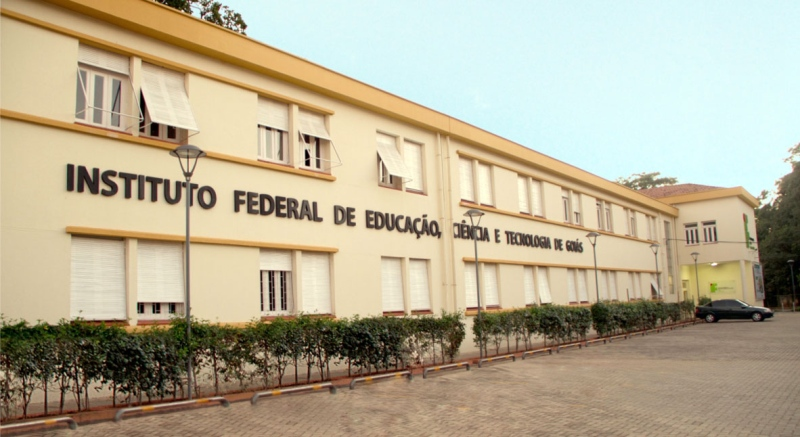
\includegraphics[width=0.40\textwidth]{./fig/foto-ifg}
  \caption{Câmpus Goiânia do IFG.}
  \label{fig:exemploFig3}
\end{figure}
\fontefig{\cite{ifg2020}}
\end{verbatim}

\begin{figure}[ht!]
 \centering
  \includegraphics[width=0.30\textwidth]{./fig/logo-ifg-vertical-goiania}
 \caption{Logo IFG.}
 \label{fig:exemploFig1}
\fontefig{\cite{ifg2020}}
\end{figure}

\begin{figure}[ht!]
 \centering
 \includegraphics[width=0.60\textwidth]{./fig/logo-ifg}
 \caption{Esta figura é um exemplo de um rótulo de figura que ocupa mais de uma linha, devendo ser identado e justificado.}
 \label{fig:exemploFig2}
\fontefig{\cite{ifg2020}}
\end{figure}

\begin{figure}[H]
 \centering
  \includegraphics[width=0.70\textwidth]{./fig/foto-ifg}
  \caption{Câmpus Goiânia do IFG.}
 \label{fig:exemploFig3}
\fontefig{\cite{ifg2020}}
\end{figure}

\subsection{Subfiguras}
\label{subsec:subfigs} 

A classe \verb|subfigure| pode ser usada para a inclusão de figuras dentro de figuras (consulte a documentação da classe para maiores detalhes). Por exemplo, a Figura \ref{fig:subfiguras} contém duas subfiguras. Estas podem ser referencidas por rótulos independentes, ou seja, podem ser referenciadas como Figuras \ref{subfig:ex1} e \ref{subfig:ex2} ou Subfiguras \subref{subfig:ex1} e \subref{subfig:ex2}.
\begin{figure}[ht!]
 \centering
%   \subfigure[][Primeira subfigura.]
  \subfigure[][Primeira subfigura.]
   {
    \includegraphics[width=0.35\textwidth]{./fig/triangulo}
    \label{subfig:ex1}
   } \qquad
  \subfigure[Segunda subfigura.]
   {
    \includegraphics[width=0.30\textwidth]{./fig/quadrado}
    \label{subfig:ex2}
   }
   \caption{{\subref{subfig:ex1}} e {\subref{subfig:ex2}} representam dois exemplos do uso de subfiguras dentro de uma única figura.}
  \label{fig:subfiguras}
\fontefig{Elaborado pelo autor}
\end{figure}

A figura \ref{fig:subfiguras} foi incluída com os comandos listados a seguir. Observe que há rótulos independentes para cada uma das subfiguras e um rótulo geral para a figura, os quais podem ser todos referenciados. Dessa forma, os textos \aspas{Figuras \ref{subfig:ex1} e \ref{subfig:ex2}} ou \aspas{Subfiguras \subref{subfig:ex1} e \subref{subfig:ex2}} podem ser gerados utilizando os códigos \verb|Figuras \ref{subfig:ex1} e \ref{subfig:ex2}| ou \verb|Subfiguras \subref{subfig:ex1} e \subref{subfig:ex2}|.

\begin{verbatim}
\begin{figure}[ht!]
 \centering
  \subfigure[Primeira subfigura.]
   {
    \includegraphics[width=0.35\textwidth]{./fig/exemploFig1}
    \label{subfig:ex1}
   } \qquad
  \subfigure[Segunda subfigura.]
   {
    \includegraphics[width=0.30\textwidth]{./fig/exemploFig2}
    \label{subfig:ex2}
   }
   \caption{{\subref{subfig:ex1}} e {\subref{subfig:ex2}} representam
             dois exemplos do uso de subfiguras dentro de uma única
             figura.}
  \label{fig:subfiguras}
  \fontefig{Elaborado pelo autor}
\end{figure}
\end{verbatim}

\subsection{Figuras usando o pacote TikZ}

Figuras podem ser desenhadas diretamente em \LaTeX\ usando o pacote TikZ. Inicialmente é preciso definir o código da figura em um arquivo com a extensão \verb|tikz| que deve ser colocado na pasta \verb|fig|. Em seguida, a figura é inserida usando o comando \verb|inputTikZ| com o tamanho da figura.

Como exemplo, a Figura \ref{fig:tikz} foi inserida usando o código a seguir.

\begin{verbatim}
\begin{figure}[!ht]
 \centering
\inputTikZ{0.6}{./fig/exemplo.tikz}
\caption{Exemplo de figura usando o pacote TikZ.}
\label{fig:tikz}
\fontefig{Elaborada pelo autor}
\end{figure}
\end{verbatim}

\begin{figure}[!ht]
 \centering
\inputTikZ{0.6}{./fig/exemplo.tikz}
\caption{Exemplo de figura usando o pacote TikZ.}
\label{fig:tikz}
\fontefig{Elaborada pelo autor}
\end{figure}

O conteúdo do arquivo \verb|exemplo.tikz| é dado a seguir.

\begin{verbatim}
\begin{tikzpicture}[->,>=stealth',shorten >=1pt,auto,
node distance=3.8cm,thick,main node/.style={circle,draw,
font=\sffamily\bfseries,align=center,text width={1.5cm}}]

  \node[main node] (b) {$b$};
  \node[main node] (sales) [right of=b] {Depart. vendas};
  \node[main node] (ands1) [right of=sales,
  font=\sffamily\it] {\textit{AND$^s$}};
  \node[main node] (inventory) [above right of=ands1] 
  {Geren. invent{\'a}rio};
  \node[main node] (freight) [below right of=ands1] 
  {Escalon. de frete};
  \node[main node] (andj1) [below right of=inventory,
  font=\sffamily\it] {\textit{AND$^j$}};
  \node[main node] (crm) [below of=sales, 
  node distance=7.8cm] {CRM};
  \node[main node] (xors1) [right of=crm,
  font=\sffamily\it] {\textit{XOR$^s$}};
  \node[main node] (bank) [above right of=xors1] 
  {Sistema banc{\'a}rio};
  \node[main node] (payment) [below right of=xors1] 
  {Sistema pagamento};
  \node[main node] (xorj1) [below right of=bank,
  font=\sffamily\it] {\textit{XOR$^j$}};
  \node[main node, accepting, node distance=2.5cm] 
  (z) [right of=xorj1] {$z$};

  \path[every node/.style={font=\sffamily\small},
  align=center]
    (b) 			edge node {Submeter\\pedido} (sales)
    (sales) 		edge node {} (ands1)
    (sales) 		edge node [left] {Processar ordem\\ 
    de pagamento} (crm)
    (ands1) 		edge [bend left] node [above left]
    {Processar\\pedido} (inventory)
    (ands1) 		edge [bend right] node [below left] 
    {Escalonar\\frete} (freight)
    (inventory) 	edge [bend left] node {} (andj1)
    (freight) 		edge [bend right] node {} (andj1)
    (crm) 			edge node {} (xors1)
    (xors1) 		edge [bend left] node [above left] 
    {Enviar\\cobran\c{c}a\\: $p=0.3$} (bank)
    (xors1) 		edge [bend right] node [below left] 
    {Processar ordem\\ de pagamento\\: $p=0.7$} 
    (payment)
    (bank) 			edge [bend left] node {} (xorj1)
    (payment) 		edge [bend right] node {} (xorj1)
    (xorj1) 		edge node {} (z);
    
%\node[draw=none] at (0.0,-2.0) {$\lambda = 65$};
\end{tikzpicture}
\end{verbatim}
 
 %% - - - - - - - - - - - - - - - - - - - - - - - - - - - - - - - - -
\section{Tabelas}
\label{sec:tabs} 

Em tabelas, deve-se evitar usar cor de fundo diferente do branco e o uso de linhas grossas ou duplas. Ao relatar dados empíricos, não se deve usar mais dígitos decimais do aqueles que possam ser garantidos pela sua precisão e reprodutibilidade. Rótulos de tabelas devem ser colocados
antes das mesmas (veja a Tabela \ref{tab:MarcMNem}).

\begin{table}[ht!]
\caption{Conteúdo do diretório}
\label{tab:MarcMNem} 
\begin{center}
\begin{tabular}{c|c|c|c|c|c|c}
\hline Tag & Comprimento & Início &   & Tag & Comprimento & Início \\ 
\hline 001 & 0020 & 00000 && 100 & 0032 & 00235\\ 
\hline 003 & 0004 & 00020 && 245 & 0087 & 00267\\ 
\hline 005 & 0017 & 00024 && 246 & 0036 & 00354\\ 
\hline 008 & 0041 & 00041 && 250 & 0012 & 00390\\ 
\hline 010 & 0024 & 00082 && 260 & 0037 & 00402\\ 
\hline 020 & 0025 & 00106 && 300 & 0029 & 00439\\ 
\hline 020 & 0044 & 00131 && 500 & 0042 & 00468\\ 
\hline 040 & 0018 & 00175 && 520 & 0220 & 00510\\ 
\hline 050 & 0024 & 00193 && 650 & 0033 & 00730\\ 
\hline 082 & 0018 & 00217 && 650 & 0012 & 00763\\ 
\hline 
\end{tabular} 
\end{center}
\fontetab{\cite{Arm1979}}
\end{table}

A Tabela \ref{tab:MarcMNem} foi gerada usando o código a seguir.

\begin{verbatim}
\begin{table}[ht!]
\caption{Conteúdo do diretório}
\label{tab:MarcMNem} 
\begin{center}
\begin{tabular}{c|c|c|c|c|c|c}
\hline Tag & Comprimento & Início &   & Tag & Comprimento & Início \\ 
\hline 001 & 0020 & 00000 && 100 & 0032 & 00235\\ 
\hline 003 & 0004 & 00020 && 245 & 0087 & 00267\\ 
\hline 005 & 0017 & 00024 && 246 & 0036 & 00354\\ 
\hline 008 & 0041 & 00041 && 250 & 0012 & 00390\\ 
\hline 010 & 0024 & 00082 && 260 & 0037 & 00402\\ 
\hline 020 & 0025 & 00106 && 300 & 0029 & 00439\\ 
\hline 020 & 0044 & 00131 && 500 & 0042 & 00468\\ 
\hline 040 & 0018 & 00175 && 520 & 0220 & 00510\\ 
\hline 050 & 0024 & 00193 && 650 & 0033 & 00730\\ 
\hline 082 & 0018 & 00217 && 650 & 0012 & 00763\\ 
\hline 
\end{tabular} 
\end{center}
\fontetab{\cite{Arm1979}}
\end{table}
\end{verbatim}

O ambiente \verb|tabular| é usado para digitar tabelas. Para ficar mais claro sobre como funciona, a seguir está uma descrição de cada comando.

\begin{verbatim}
{c|c|c|c|c|c|c}
\end{verbatim}

Isso declara que sete colunas, separadas por uma linha vertical, serão usadas na tabela. Cada \verb|c| significa que o conteúdo da coluna será centralizado, você também pode usar \verb|r| para alinhar o texto à direita e \verb|l| para o alinhamento à esquerda.

\begin{verbatim}
\hline
\end{verbatim}

Isso irá inserir uma linha horizontal na tabela. Não há restrição quanto ao número de vezes que você pode usar \verb|\hline|.

\begin{verbatim}
cell1 & cell2 & cell3 & cell4 & cell5 & cell6 & cell7 \\
\end{verbatim}

Cada \& é um separador de células e a barra invertida dupla $\backslash\backslash$ define o final desta linha.

Outro exemplo é representado pela Tabela \ref{tab:outro}. O código para gerá-la é apresentado a seguir.

\begin{verbatim}
\begin{table}[h!]
\caption{Outro exemplo de tabela}
\label{tab:outro}
\renewcommand{\baselinestretch}{1.2}% for tabular environment
\small
\begin{center}
\begin{tabular}{cccccc}
\hline
   & \multirow{2}{22mm}{\renewcommand{\baselinestretch}{0.7}
   \small\centering Quantitative measures} & \multicolumn{4}{c}{Markers} 
   \\ \cline{3-6}
   & & \multicolumn{1}{c}{RO} & \multicolumn{1}{c}{ASF} & 
   \multicolumn{1}{c}{ISO} & \multicolumn{1}{c}{ADF} \\ \hline
   \multirow{3}{20mm}{\renewcommand{\baselinestretch}{0.7}
   \small\centering Test image scale 2}
& RMSE & 0.126 & 0.187 & 0.118 & 0.103 \\
& NMSE & 0.046 & 0.101 & 0.040 & 0.031 \\
& SSIM & 0.9981 & 0.9956 & 0.9984 & 0.9989 \\ \hline
   \multirow{3}{18mm}{\renewcommand{\baselinestretch}{0.7}\small
   \centering Cameraman scale 4}
& RMSE & 13.748 & 15.649 & 10.132 & 4.325 \\
& NMSE & 0.011 & 0.014 & 0.006 & 0.001 \\
& SSIM & 0.923 & 0.847 & 0.904 & 0.933 \\ \hline
\end{tabular}
\end{center}
\fontetab{Referência à fonte da tabela.}
\end{table}
\end{verbatim}

\begin{table}[h!]
\caption{Outro exemplo de tabela}
\label{tab:outro}
\renewcommand{\baselinestretch}{1.2}% for tabular environment
\small
\begin{center}
\begin{tabular}{cccccc}
\hline
   & \multirow{2}{22mm}{\renewcommand{\baselinestretch}{0.7}\small\centering Quantitative measures} & \multicolumn{4}{c}{Markers} \\ \cline{3-6}
   & & \multicolumn{1}{c}{RO} & \multicolumn{1}{c}{ASF} & \multicolumn{1}{c}{ISO} & \multicolumn{1}{c}{ADF} \\ \hline
   \multirow{3}{20mm}{\renewcommand{\baselinestretch}{0.7}\small\centering Test image scale 2}
& RMSE & 0.126 & 0.187 & 0.118 & 0.103 \\
& NMSE & 0.046 & 0.101 & 0.040 & 0.031 \\
& SSIM & 0.9981 & 0.9956 & 0.9984 & 0.9989 \\ \hline
   \multirow{3}{18mm}{\renewcommand{\baselinestretch}{0.7}\small\centering Cameraman scale 4}
& RMSE & 13.748 & 15.649 & 10.132 & 4.325 \\
& NMSE & 0.011 & 0.014 & 0.006 & 0.001 \\
& SSIM & 0.923 & 0.847 & 0.904 & 0.933 \\ \hline
\end{tabular}
\end{center}
\fontetab{Referência à fonte da tabela.}
\end{table}

Mais um exemplo de tabela é dado pela Tabela \ref{tab:maisum}, cujo código é apresentado a seguir.

\begin{verbatim}
\begin{table}[!ht]
\caption{Mais um exemplo de tabela}
\label{tab:maisum}
\renewcommand{\baselinestretch}{1.2}% for tabular environment
\small
\begin{center}
\begin{tabular}{ccccc}
\hline
\multirow{4}{16mm}{\renewcommand{\baselinestretch}{0.7}
\small\centering Leveling's Scale} & \multicolumn{4}{c}
{Values for the scale relation of the four different type of markers} 
\\ \cline{2-5}
& \multirow{3}{29mm}{\renewcommand{\baselinestretch}{1}\small
\centering Structure element's size $r$ for RO and ASF} & 
\multicolumn{2}{c}{Isotropic diffusion} & 
\multirow{3}{20mm}{\renewcommand{\baselinestretch}{1}\small
\centering Anisotropic diffusion iterations $t$} \\ \cline{3-4}
& & \multirow{2}{23mm}{\renewcommand{\baselinestretch}{0.7}
\small\centering Standard deviation $\sigma$} & \multirow{2}{12mm}
{\renewcommand{\baselinestretch}{0.7}\small\centering Kernel size} & \\
& & & & \\ \hline
1 & 1 & 0.5 & $5 \times 5$ & 100 \\
2 & 2 & 1.0 & $7 \times 7$ & 200 \\
3 & 3 & 1.5 & $11 \times 11$ & 300 \\
4 & 4 & 2.0 & $13 \times 13$ & 400 \\
5 & 5 & 2.5 & $17 \times 17$ & 500 \\
6 & 6 & 3.0 & $19 \times 19$ & 600 \\
7 & 7 & 3.5 & $23 \times 23$ & 700 \\ \hline
\end{tabular}
\end{center}
\fontetab{Referência à fonte da tabela.}
\end{table} 
\end{verbatim}

\begin{table}[!ht]
\caption{Mais um exemplo de tabela}
\label{tab:maisum}
\renewcommand{\baselinestretch}{1.2}% for tabular environment
\small
\begin{center}
\begin{tabular}{ccccc}
\hline
\multirow{4}{16mm}{\renewcommand{\baselinestretch}{0.7}\small\centering Leveling's Scale} & \multicolumn{4}{c}{Values for the scale relation of the four different type of markers} \\ \cline{2-5}
& \multirow{3}{29mm}{\renewcommand{\baselinestretch}{1}\small\centering Structure element's size $r$ for RO and ASF} & \multicolumn{2}{c}{Isotropic diffusion} & \multirow{3}{20mm}{\renewcommand{\baselinestretch}{1}\small\centering Anisotropic diffusion iterations $t$} \\ \cline{3-4}
& & \multirow{2}{23mm}{\renewcommand{\baselinestretch}{0.7}\small\centering Standard deviation $\sigma$} & \multirow{2}{12mm}{\renewcommand{\baselinestretch}{0.7}\small\centering Kernel size} & \\
& & & & \\ \hline
1 & 1 & 0.5 & $5 \times 5$ & 100 \\
2 & 2 & 1.0 & $7 \times 7$ & 200 \\
3 & 3 & 1.5 & $11 \times 11$ & 300 \\
4 & 4 & 2.0 & $13 \times 13$ & 400 \\
5 & 5 & 2.5 & $17 \times 17$ & 500 \\
6 & 6 & 3.0 & $19 \times 19$ & 600 \\
7 & 7 & 3.5 & $23 \times 23$ & 700 \\ \hline
\end{tabular}
\end{center}
\fontetab{Referência à fonte da tabela.}
\end{table} 

A Tabela \ref{tab:longas} é um exemplo de tabela longa que ocupa várias páginas. O código para incluí-la é apresentado a seguir, sendo omitido parte das linhas da tabela gerada.

\begin{verbatim}
\setlongtables
\begin{longtable}[c]{c|c|c|c|c|c}
\caption{Exemplo de tabela longa que atravessa várias páginas.}
\label{tab:longas}\\
\hline
\textbf{Campo1} & \textbf{Campo2} & \textbf{Campo3} & 
\textbf{Campo4} & \textbf{Campo5} & \textbf{Campo6} \\
\hline\hline
\endfirsthead
\caption[]{Continuação} \\
\hline
\textbf{Campo1} & \textbf{Campo2} & \textbf{Campo3} & 
\textbf{Campo4} & \textbf{Campo5} & \textbf{Campo6} \\
\hline\hline
\endhead
\hline\hline
\endlastfoot
\hline
\multicolumn{6}{r}{\captionlabelfont\captionsize(Continua)}\\
\endfoot
	campo1 & campo2 & campo3 & campo4 & campo5 & campo6 \\
	...
	campo1 & campo2 & campo3 & campo4 & campo5 & campo6 \\
\hline
\end{longtable}
% o comando \fontetab{} não pode ser usado neste caso
\vspace{-8mm}
\begin{center}
\footnotesize
Fonte: Referência a fonte da tabela.
\end{center}
\end{verbatim}

\setlongtables
\begin{longtable}[c]{c|c|c|c|c|c}
\caption{Exemplo de tabela longa que atravessa várias páginas.}
\label{tab:longas}\\
\hline
\textbf{Campo1} & \textbf{Campo2} & \textbf{Campo3} & \textbf{Campo4} & \textbf{Campo5} & \textbf{Campo6} \\
\hline\hline
\endfirsthead
\caption[]{Continuação} \\
\hline
\textbf{Campo1} & \textbf{Campo2} & \textbf{Campo3} & \textbf{Campo4} & \textbf{Campo5} & \textbf{Campo6} \\
\hline\hline
\endhead
\hline\hline
\endlastfoot
\hline
\multicolumn{6}{r}{\captionlabelfont\captionsize(Continua)}\\
\endfoot
	campo1 & campo2 & campo3 & campo4 & campo5 & campo6 \\
	campo1 & campo2 & campo3 & campo4 & campo5 & campo6 \\
	campo1 & campo2 & campo3 & campo4 & campo5 & campo6 \\
	campo1 & campo2 & campo3 & campo4 & campo5 & campo6 \\
	campo1 & campo2 & campo3 & campo4 & campo5 & campo6 \\
	campo1 & campo2 & campo3 & campo4 & campo5 & campo6 \\
	campo1 & campo2 & campo3 & campo4 & campo5 & campo6 \\
	campo1 & campo2 & campo3 & campo4 & campo5 & campo6 \\
	campo1 & campo2 & campo3 & campo4 & campo5 & campo6 \\
	campo1 & campo2 & campo3 & campo4 & campo5 & campo6 \\
	campo1 & campo2 & campo3 & campo4 & campo5 & campo6 \\
	campo1 & campo2 & campo3 & campo4 & campo5 & campo6 \\
	campo1 & campo2 & campo3 & campo4 & campo5 & campo6 \\
	campo1 & campo2 & campo3 & campo4 & campo5 & campo6 \\
	campo1 & campo2 & campo3 & campo4 & campo5 & campo6 \\
	campo1 & campo2 & campo3 & campo4 & campo5 & campo6 \\
	campo1 & campo2 & campo3 & campo4 & campo5 & campo6 \\
	campo1 & campo2 & campo3 & campo4 & campo5 & campo6 \\
	campo1 & campo2 & campo3 & campo4 & campo5 & campo6 \\
	campo1 & campo2 & campo3 & campo4 & campo5 & campo6 \\
	campo1 & campo2 & campo3 & campo4 & campo5 & campo6 \\
	campo1 & campo2 & campo3 & campo4 & campo5 & campo6 \\
	campo1 & campo2 & campo3 & campo4 & campo5 & campo6 \\
	campo1 & campo2 & campo3 & campo4 & campo5 & campo6 \\
	campo1 & campo2 & campo3 & campo4 & campo5 & campo6 \\
	campo1 & campo2 & campo3 & campo4 & campo5 & campo6 \\
	campo1 & campo2 & campo3 & campo4 & campo5 & campo6 \\
	campo1 & campo2 & campo3 & campo4 & campo5 & campo6 \\
	campo1 & campo2 & campo3 & campo4 & campo5 & campo6 \\
	campo1 & campo2 & campo3 & campo4 & campo5 & campo6 \\
	campo1 & campo2 & campo3 & campo4 & campo5 & campo6 \\
	campo1 & campo2 & campo3 & campo4 & campo5 & campo6 \\
	campo1 & campo2 & campo3 & campo4 & campo5 & campo6 \\
	campo1 & campo2 & campo3 & campo4 & campo5 & campo6 \\
	campo1 & campo2 & campo3 & campo4 & campo5 & campo6 \\
	campo1 & campo2 & campo3 & campo4 & campo5 & campo6 \\
	campo1 & campo2 & campo3 & campo4 & campo5 & campo6 \\
	campo1 & campo2 & campo3 & campo4 & campo5 & campo6 \\
	campo1 & campo2 & campo3 & campo4 & campo5 & campo6 \\
	campo1 & campo2 & campo3 & campo4 & campo5 & campo6 \\
	campo1 & campo2 & campo3 & campo4 & campo5 & campo6 \\
	campo1 & campo2 & campo3 & campo4 & campo5 & campo6 \\
	campo1 & campo2 & campo3 & campo4 & campo5 & campo6 \\
	campo1 & campo2 & campo3 & campo4 & campo5 & campo6 \\
	campo1 & campo2 & campo3 & campo4 & campo5 & campo6 \\
	campo1 & campo2 & campo3 & campo4 & campo5 & campo6 \\
	campo1 & campo2 & campo3 & campo4 & campo5 & campo6 \\
	campo1 & campo2 & campo3 & campo4 & campo5 & campo6 \\
	campo1 & campo2 & campo3 & campo4 & campo5 & campo6 \\
	campo1 & campo2 & campo3 & campo4 & campo5 & campo6 \\
	campo1 & campo2 & campo3 & campo4 & campo5 & campo6 \\
	campo1 & campo2 & campo3 & campo4 & campo5 & campo6 \\
	campo1 & campo2 & campo3 & campo4 & campo5 & campo6 \\
	campo1 & campo2 & campo3 & campo4 & campo5 & campo6 \\
	campo1 & campo2 & campo3 & campo4 & campo5 & campo6 \\
	campo1 & campo2 & campo3 & campo4 & campo5 & campo6 \\
	campo1 & campo2 & campo3 & campo4 & campo5 & campo6 \\
	campo1 & campo2 & campo3 & campo4 & campo5 & campo6 \\
	campo1 & campo2 & campo3 & campo4 & campo5 & campo6 \\
	campo1 & campo2 & campo3 & campo4 & campo5 & campo6 \\
	campo1 & campo2 & campo3 & campo4 & campo5 & campo6 \\
	campo1 & campo2 & campo3 & campo4 & campo5 & campo6 \\
	campo1 & campo2 & campo3 & campo4 & campo5 & campo6 \\
	campo1 & campo2 & campo3 & campo4 & campo5 & campo6 \\
	campo1 & campo2 & campo3 & campo4 & campo5 & campo6 \\
	campo1 & campo2 & campo3 & campo4 & campo5 & campo6 \\
	campo1 & campo2 & campo3 & campo4 & campo5 & campo6 \\
	campo1 & campo2 & campo3 & campo4 & campo5 & campo6 \\
	campo1 & campo2 & campo3 & campo4 & campo5 & campo6 \\
	campo1 & campo2 & campo3 & campo4 & campo5 & campo6 \\
	campo1 & campo2 & campo3 & campo4 & campo5 & campo6 \\
	campo1 & campo2 & campo3 & campo4 & campo5 & campo6 \\
	campo1 & campo2 & campo3 & campo4 & campo5 & campo6 \\
\hline
\end{longtable}
% o comando \fontetab{} não pode ser usado neste caso
\vspace{-8mm}
\begin{center}
\footnotesize
Fonte: Referência a fonte da tabela.
\end{center}

A \autoref{tab:longa} é um exemplo de tabela no modo paisagem e que ocupa também várias páginas. O código para incluí-la é apresentado a seguir, sendo omitido parte das linhas da tabela gerada.

\begin{verbatim}
\setlongtables
\begin{landscape}
\begin{longtable}[c]{c|c|c|c|c|c|c|c|c|c}
\caption{Exemplo de tabela longa, em paisagem, que atravessa 
várias páginas.}\label{tab:longa}\\
\hline
\textbf{BOX1} & \textbf{BOX2} & \textbf{BOX3} & \textbf{BOX4} & 
\textbf{BOX5} & \textbf{BOX6} & \textbf{BOX7} & \textbf{BOX8} & 
\textbf{BOX9} & \textbf{BOX10} \\
\hline\hline
\endfirsthead
\caption[]{Conclusão}\\
\hline
\textbf{BOX1} & \textbf{BOX2} & \textbf{BOX3} & \textbf{BOX4} & 
\textbf{BOX5} & \textbf{BOX6} & \textbf{BOX7} & \textbf{BOX8} & 
\textbf{BOX9} & \textbf{BOX10} \\
\hline\hline
\endhead
\endlastfoot
\hline
\multicolumn{10}{r}{\captionlabelfont\captionsize(Continua)}\\
\endfoot
	
	BOX1 & BOX2 & BOX3 & BOX4 & BOX5 & BOX6 & BOX7 & BOX8 
	& BOX9 & BOX10 \\
	...
	BOX1 & BOX2 & BOX3 & BOX4 & BOX5 & BOX6 &	BOX7 & BOX8 
	& BOX9 & BOX10 \\
\hline
\end{longtable}
\vspace{-8mm}
% o comando \fontetab{} não pode ser usado neste caso
\begin{center}
\footnotesize
Fonte: Referência a fonte da tabela.
\end{center}
\end{landscape}

\end{verbatim}

\setlongtables
\begin{landscape}
\begin{longtable}[c]{c|c|c|c|c|c|c|c|c|c}
\caption{Exemplo de tabela longa, em paisagem, que atravessa várias páginas.}\label{tab:longa}\\
\hline
\textbf{BOX1} & \textbf{BOX2} & \textbf{BOX3} & \textbf{BOX4} & \textbf{BOX5} & \textbf{BOX6} & \textbf{BOX7} & \textbf{BOX8} & \textbf{BOX9} & \textbf{BOX10} \\
\hline\hline
\endfirsthead
\caption[]{Conclusão}\\
\hline
\textbf{BOX1} & \textbf{BOX2} & \textbf{BOX3} & \textbf{BOX4} & \textbf{BOX5} & \textbf{BOX6} & \textbf{BOX7} & \textbf{BOX8} & \textbf{BOX9} & \textbf{BOX10} \\
\hline\hline
\endhead
\endlastfoot
\hline
\multicolumn{10}{r}{\captionlabelfont\captionsize(Continua)}\\
\endfoot
	
	BOX1 & BOX2 & BOX3 & BOX4 & BOX5 & BOX6 & BOX7 & BOX8 & BOX9 & BOX10 \\
	BOX1 & BOX2 & BOX3 & BOX4 & BOX5 & BOX6 & BOX7 & BOX8 & BOX9 & BOX10 \\
	BOX1 & BOX2 & BOX3 & BOX4 & BOX5 & BOX6 & BOX7 & BOX8 & BOX9 & BOX10 \\
	BOX1 & BOX2 & BOX3 & BOX4 & BOX5 & BOX6 &	BOX7 & BOX8 & BOX9 & BOX10 \\
	BOX1 & BOX2 & BOX3 & BOX4 & BOX5 & BOX6 &	BOX7 & BOX8 & BOX9 & BOX10 \\
	BOX1 & BOX2 & BOX3 & BOX4 & BOX5 & BOX6 &	BOX7 & BOX8 & BOX9 & BOX10 \\
	BOX1 & BOX2 & BOX3 & BOX4 & BOX5 & BOX6 &	BOX7 & BOX8 & BOX9 & BOX10 \\
	BOX1 & BOX2 & BOX3 & BOX4 & BOX5 & BOX6 &	BOX7 & BOX8 & BOX9 & BOX10 \\
	BOX1 & BOX2 & BOX3 & BOX4 & BOX5 & BOX6 &	BOX7 & BOX8 & BOX9 & BOX10 \\
	BOX1 & BOX2 & BOX3 & BOX4 & BOX5 & BOX6 &	BOX7 & BOX8 & BOX9 & BOX10 \\
	BOX1 & BOX2 & BOX3 & BOX4 & BOX5 & BOX6 & BOX7 & BOX8 & BOX9 & BOX10 \\
	BOX1 & BOX2 & BOX3 & BOX4 & BOX5 & BOX6 &	BOX7 & BOX8 & BOX9 & BOX10 \\
	BOX1 & BOX2 & BOX3 & BOX4 & BOX5 & BOX6 &	BOX7 & BOX8 & BOX9 & BOX10 \\
	BOX1 & BOX2 & BOX3 & BOX4 & BOX5 & BOX6 &	BOX7 & BOX8 & BOX9 & BOX10 \\
	BOX1 & BOX2 & BOX3 & BOX4 & BOX5 & BOX6 &	BOX7 & BOX8 & BOX9 & BOX10 \\
	BOX1 & BOX2 & BOX3 & BOX4 & BOX5 & BOX6 &	BOX7 & BOX8 & BOX9 & BOX10 \\
	BOX1 & BOX2 & BOX3 & BOX4 & BOX5 & BOX6 &	BOX7 & BOX8 & BOX9 & BOX10 \\
	BOX1 & BOX2 & BOX3 & BOX4 & BOX5 & BOX6 &	BOX7 & BOX8 & BOX9 & BOX10 \\
	BOX1 & BOX2 & BOX3 & BOX4 & BOX5 & BOX6 &	BOX7 & BOX8 & BOX9 & BOX10 \\                                 
	BOX1 & BOX2 & BOX3 & BOX4 & BOX5 & BOX6 &	BOX7 & BOX8 & BOX9 & BOX10 \\
	BOX1 & BOX2 & BOX3 & BOX4 & BOX5 & BOX6 &	BOX7 & BOX8 & BOX9 & BOX10 \\
	BOX1 & BOX2 & BOX3 & BOX4 & BOX5 & BOX6 &	BOX7 & BOX8 & BOX9 & BOX10 \\
	BOX1 & BOX2 & BOX3 & BOX4 & BOX5 & BOX6 &	BOX7 & BOX8 & BOX9 & BOX10 \\
	BOX1 & BOX2 & BOX3 & BOX4 & BOX5 & BOX6 &	BOX7 & BOX8 & BOX9 & BOX10 \\
	BOX1 & BOX2 & BOX3 & BOX4 & BOX5 & BOX6 &	BOX7 & BOX8 & BOX9 & BOX10 \\
	BOX1 & BOX2 & BOX3 & BOX4 & BOX5 & BOX6 &	BOX7 & BOX8 & BOX9 & BOX10 \\
	BOX1 & BOX2 & BOX3 & BOX4 & BOX5 & BOX6 &	BOX7 & BOX8 & BOX9 & BOX10 \\
	BOX1 & BOX2 & BOX3 & BOX4 & BOX5 & BOX6 &	BOX7 & BOX8 & BOX9 & BOX10 \\
\hline
\end{longtable}
\vspace{-8mm}
% o comando \fontetab{} não pode ser usado neste caso
\begin{center}
\footnotesize
Fonte: Referência a fonte da tabela.
\end{center}
\end{landscape}

%% - - - - - - - - - - - - - - - -- - - - - - - - - - - - - - - - - -
\section{Algoritmos}
\label{sec:algor} 
Algoritmos devem ser representados no formato do Algoritmo \ref{alg:poten}, que foi descrito com o uso da classe \textsf{algorithm2e}. A rigor não é obrigatório o uso dessa classe, contudo o uso da mesma permite que seja gerada automaticamente uma lista de algoritmos.

\medskip
\begin{center}
\begin{minipage}{0.92\textwidth}
\begin{algorithm2e}[H]
 \DontPrintSemicolon
 \LinesNumbered
 \SetAlgoLined
 \BlankLine
 \Entrada{vetor $A[i\,.\,.\,j]$, inteiros não negativos $i$ e $j$.}
 \Saida{vetor $A[i\,.\,.\,j]$ ordenado.}
 \BlankLine
 $n \leftarrow j - i$.\;
 \eSe{$(n<4)$}
   {Ordene com $\leq 3$ comparações.}
   {Divida $A$ em $\lceil\sqrt{n}\,\,\rceil$ subvetores de comprimento máximo $\lfloor\sqrt{n}\,\rfloor$.\;
    Aplique $MSR$ a cada um dos subvetores.\;
    Intercale os subvetores.\;}
\caption{$MSR(A,i,j)$ \label {alg:poten}}
\end{algorithm2e}
\end{minipage}
\end{center}

O código utilizado para gerar o algoritmo é apresentado a seguir. A lista completa de palavras-chave é apresentada no Apêndice \ref{apend:algorithm2e}.

\begin{verbatim}
\medskip
\begin{center}
\begin{minipage}{0.92\textwidth}
\begin{algorithm2e}[H]
 \DontPrintSemicolon
 \LinesNumbered
 \SetAlgoLined
 \BlankLine
 \Entrada{vetor $A[i\,.\,.\,j]$, inteiros não negativos $i$ e $j$.}
 \Saida{vetor $A[i\,.\,.\,j]$ ordenado.}
 \BlankLine
 $n \leftarrow j - i$.\;
 \eSe{$(n<4)$}
   {Ordene com $\leq 3$ comparações.}
   {Divida $A$ em $\lceil\sqrt{n}\,\,\rceil$ subvetores de 
   comprimento máximo $\lfloor\sqrt{n}\,\rfloor$.\;
    Aplique $MSR$ a cada um dos subvetores.\;
    Intercale os subvetores.\;}
\caption{$MSR(A,i,j)$ \label {alg:poten}}
\end{algorithm2e}
\end{minipage}
\end{center}
\end{verbatim}

%% - - - - - -  - - - - - - - - - - - - - - - - - - - - - - - - - - -
\section{Códigos de Programa}
\label{sec:progs} 

Códigos de programa podem ser importados, mantendo-se a formatação original, conforme se pode ver no exemplo do Código \ref{code:prog1}. Este exemplo usa o ambiente \textsf{codigo}, definido na \textsf{classe-ifg}, que permite que uma lista de programas seja gerada automaticamente.

Para inserir o código coloque na pasta \verb|prog| o arquivo com o conteúdo a ser inserido. Depois utilize o código a seguir. Atualmente a \textsf{classe-ifg} permite formatar códigos das linguagens XML, Java, Matlab e Python.

\begin{verbatim}
\begin{center}
 \begin{codigo}[H]
   \small
   \lstinputlisting[language=Matlab]{prog/retangular.m}
   \caption{\texttt{funcao\_retangular()} }
   \label{code:prog1}
  \end{codigo}
\end{center}
\end{verbatim}

%% - - - - - - - - - - - - - - - - - - - - - - - - - - - - - - - - - - -
\section{Teoremas, Corolários e Demonstrações}
\label{sec:teor}
 O uso do ambiente \textsf{theorem} permite a escrita de teoremas, como no exemplo a seguir:
\begin{verbatim}
\begin{theorem}[Pitágoras]
Em todo triângulo retângulo o quadrado do comprimento
da hipotenusa é igual a soma dos quadrados dos
comprimentos dos catetos.
\end{theorem}
\end{verbatim}

O resultado é o mostrado a seguir:

\begin{theorem}[Pitágoras]
Em todo triângulo retângulo o quadrado do comprimento da hipotenusa é igual a soma dos quadrados dos comprimentos dos catetos.
\end{theorem}

Da mesma forma pode-se usar o ambiente \textsf{proof} para demonstrações de teoremas:
\begin{verbatim}
\begin{proof}
Para demonstrar o Teorema de Pitágoras \dots
\end{proof}
\end{verbatim}

Neste caso, o resultado é:
\begin{proof}
Para demonstrar o Teorema de Pitágoras \dots
\end{proof}

Além desses dois ambientes, estão definidos os ambientes \textsf{definition} (Definição), \textsf{corollary} (Corolário), \textsf{lemma} (Lema)), \textsf{proposition} (Proposição), \textsf{comment} (Observação).

%% - - - - - - - - - - - - - - - - - - - - - - - - - - - - - - - - -
\section{Referências e citações}

Em documentos acadêmicos podem existir as citações podem ser: \textbf{implícitas} quando as referências não fazem parte do texto ou \textbf{explícitas} quando o autor referente a citação é mencionado explicitamente na sentença. Nesse sentido, deve-se utilizar os comandos específicos para cada tipo de citação, ou seja, em citações explicitas deve-se usar o comando \verb|citeonline{}| e nas demais situações é usado o comando\verb|cite{}|. Alguns exemplos são apresentados no \autoref{qua:exemplo-citacao}.

\begin{quadro}[!ht]
\centering
\caption{Exemplos de citações no documento}
\label{qua:exemplo-citacao}
\begin{tabular}{|c|c|}        
\hline
\textbf{Código em \LaTeX} & \textbf{Código Compilado}\\ \hline\hline
\begin{minipage}[t]{8cm}
\vspace{5pt}
\begin{verbatim}
A ironia será assim uma ... proposta
por \citeonline{10520:2000:4.1-1}.
\end{verbatim}
\vspace{5pt}
\end{minipage}
&
\begin{minipage}[t]{6cm}
\vspace{5pt}
A ironia será assim uma ... proposta 
por \citeonline{10520:2000:4.1-1}.
\vspace{5pt}
\end{minipage}\\\hline

\begin{minipage}[t]{8cm}
\vspace{5pt}
\begin{verbatim}
\citeonline[p.~146]{10520:2000:4.2-2}
dizem que ... 
\end{verbatim}
\vspace{5pt}
\end{minipage}
&
\begin{minipage}[t]{6cm}
\vspace{5pt}
\citeonline[p.~146]{10520:2000:4.2-2} dizem que {...}
\vspace{5pt}
\end{minipage}\\ \hline

\begin{minipage}[t]{8cm}
\vspace{5pt}
\begin{verbatim}
``Apesar das ... da filosofia''
\cite[p.~293]{10520:2000:4.1-2}.
\end{verbatim}
\vspace{5pt}
\end{minipage}
&
\begin{minipage}[t]{6cm}
\vspace{5pt}
``Apesar das {...} da filosofia'' \cite[p.~293]{10520:2000:4.1-2}.
\vspace{5pt}
\end{minipage} \\ \hline

\begin{minipage}[t]{8cm}
\vspace{5pt}
\begin{verbatim}
Depois, ...  que prefiro
\cite{10520:2000:4.1-3}.
\end{verbatim}
\vspace{5pt}
\end{minipage}
&
\begin{minipage}[t]{6cm}
\vspace{5pt}
Depois, {...} que prefiro \cite{10520:2000:4.1-3}.
\vspace{5pt}
\end{minipage}\\ \hline
\end{tabular}
\fontequa{\cite{icmc-usp}}
\end{quadro}

Para especificar a página, seção ou capítulo consultado na referência é preciso acrescentá-lo entre colchetes com os comandos \verb|\cite[página]{}| ou \verb|\citeonline[página]{}|. O texto colocado entre colchetes aparecerá logo após o ano. Maiores informações sobre os comandos utilizados para citação posem ser consultados no manual de referência da abnTeX2, incluindo o uso de \textbf{apud} \cite{abntex2cite-alf}.

\section{Citações Indiretas}

As citações indiretas são caracterizadas como uma espécie de paráfrase das ideias de um determinado autor, ou seja, o pesquisador, por meio de suas próprias palavras, interpreta o discurso de outrem, contudo, mantendo o mesmo sentido. Outro aspecto que deve ser considerado é a necessidade de o autor (ou os autores) e o ano em que a obra foi publicada serem mencionados. 

Nas citações indiretas há duas formatações possíveis dependendo de como ocorre a citação no texto. Quando o autor é mencionado explicitamente utiliza-se o comando \verb|\citeonline{}|, caso contrário, deve utilizar o comando \verb|cite{}|. 

\section{Citações diretas}
\label{sec-citacao}

As citações diretas ocorrem quando o texto de uma referência é transcrito literalmente. As citações diretas curtas (até três linhas) são inseridas no texto entre aspas duplas. As aspas simples são utilizadas para indicar citação no interior da citação: \aspas{Nas citações, as chamadas pelo sobrenome do autor [...] incluído na sentença devem ser em letras maiúsculas e minúsculas e, quando estiverem entre parênteses, devem ser em letras maiúsculas} \cite[sec.~5]{NBR10520:2002}.

\begin{verbatim}
``Nas citações, as chamadas pelo sobrenome do autor [...] incluído na 
sentença devem ser em letras maiúsculas e minúsculas e, quando 
estiverem entre parênteses, devem ser em letras maiúsculas''
\cite[5]{NBR10520:2002}.
\end{verbatim}

Cabe ressaltar que em \LaTeX as aspas iniciais são diferentes das finais. Para tanto, pode-se utilizar o comando \verb|\aspas{CONTEUDO}| para inserir um determinado conteúdo entre aspas.

As citações diretas longas (com mais de 3 linhas) podem ser inseridas por meio do ambiente \texttt{citacao}:

\begin{citacao}
As citações diretas, no texto, com mais de três linhas, devem ser
destacadas com recuo de 4 cm da margem esquerda, com letra menor que a do texto
utilizado e sem as aspas. No caso de documentos datilografados, deve-se
observar apenas o recuo \cite[5.3]{NBR10520:2002}.
\end{citacao}

Use o ambiente assim:

\begin{verbatim}
\begin{citacao}
As citações diretas, no texto, com mais de três linhas [...] deve-se 
observar apenas o recuo \cite[5.3]{NBR10520:2002}.
\end{citacao}
\end{verbatim}

\section{Referências Bibliográficas}

As referências bibliográficas utilizadas neste modelo estão de acordo com a Norma Brasileira ABNT 6023:2018 Informação e documentação - Referências - Elaboração \cite{abnt}. A seguir são apresentados exemplos em cada um das categorias, considerando somente os elementos essenciais. Adicionalmente, é apresentado o código \BibTeX~para geração da referência.

\subsection{Monografia no todo}\label{sec:monografia}

Inclui livro e/ou folheto (manual, guia, catálogo, enciclopédia, dicionário, entre outros) e trabalho acadêmico (tese, dissertação, trabalho de conclusão de curso, entre outros).

Os elementos essenciais para livro e/ou folheto são: autor, título, subtítulo (se houver), edição (se houver), local, editora e data de publicação. Quando necessário, acrescentam-se elementos complementares à referência para melhor identificar o documento.

EXEMPLO 1

LUCK, Heloisa. \textbf{Liderança em gestão escolar}. 4. ed. Petrópolis: Vozes, 2010.

\begin{verbatim}
@book{luck2014e,
 author = {Heloisa Luck},
 title = {Liderança em gestão escolar},
 edition = {2},
 address = {Petrópolis},
 publisher = {Vozes},
 year = {2010}
}
\end{verbatim}

EXEMPLO 2

BAUMAN, Zygmunt. \textbf{Globalização}: as consequências humanas. Rio de Janeiro: Jorge Zahar, 1999.

\begin{verbatim}
@book{bauman99,
 author = {Zygmunt Bauman},
 title = {Globalização},
 subtitle = {as consequências humanas},
 address = {Rio de Janeiro},
 publisher = {Jorge Zahar},
 year = {1999}
}
\end{verbatim}

Os elementos essenciais para trabalho acadêmico são: autor, título, subtítulo (se houver), ano de depósito, tipo do trabalho (tese, dissertação, trabalho de conclusão de curso e outros), grau (especialização, doutorado, entre outros) e curso entre parênteses, vinculação acadêmica, local e data de apresentação ou defesa. Quando necessário, acrescentam-se elementos complementares à referência para melhor identificar o documento.

EXEMPLO 1

AGUIAR, André Andrade de. \textbf{Avaliação da microbiota bucal em pacientes sob uso crônico de penicilina e benzatina}. Tese (Doutorado em Cardiologia) — Faculdade de Medicina, Universidade de São Paulo, São Paulo, 2009.

\begin{verbatim}
@phdthesis{aguiar09,
 author = {André Andrade de Aguiar},
 title = {Avaliação da microbiota bucal em pacientes sob uso crônico de penicilina e benzatina},
 year = {2009},
 type = {Doutorado em Cardiologia},
 school = {Faculdade de Medicina, Universidade de São Paulo},
 address = {São Paulo}
}
\end{verbatim}

EXEMPLO 2

ALVES, Daian Péricles. \textbf{Implementação de conceitos de manufatura colaborativa}: um projeto virtual. Trabalho de Conclusão de Curso (Bacharelado em Engenharia Industrial Mecânica) — Universidade Tecnológica Federal do Paraná, Curitiba, 2008.

\begin{verbatim}
@tcc{alves08,
 author = {Daian Péricles Alves},
 title = {Implementação de conceitos de manufatura colaborativa},
 subtitle = {um projeto virtual},
 year = {2008},
 type = {Bacharelado em Engenharia Industrial Mecânica},
 school = {Universidade Tecnológica Federal do Paraná},
 address = {Curitiba}
}
\end{verbatim}

EXEMPLO 3 

RODRIGUES, Ana Lúcia Aquilas. \textbf{Impacto de um programa de exercícios no local de trabalho sobre o nível de atividade física e o estágio de prontidão para a mudança de comportamento}. Dissertação (Mestrado em Fisiopatologia Experimental) — Faculdade de Medicina, Universidade de São Paulo, São Paulo, 2009.

\begin{verbatim}
@mastersthesis{rodrigues09,
 author = {Ana Lúcia Aquilas Rodrigues},
 title = {Impacto de um programa de exercícios no local de trabalho sobre o nível de atividade física e o estágio de prontidão para a mudança de comportamento},
 year = {2009},
 type = {Mestrado em Fisiopatologia Experimental},
 school = {Faculdade de Medicina, Universidade de São Paulo},
 address = {São Paulo}
}
\end{verbatim}

EXEMPLO 4 

PANIAGO, Cecília Yade Nogueira Alves. \textbf{A relação entre professor-aluno na educação de jovens e adultos (EJA)}. Monografia (Especialização em Docência na Educação Profissional, Técnica e Tecnológica) — Instituto Federal de Educação, Ciência e Tecnologia de Goiás, Senador Canedo, 2020.

\begin{verbatim}
@monography{paniago20,
 author = {Cecília Yade Nogueira Alves Paniago},
 title = {A relação entre professor - aluno na educação de jovens e adultos (EJA)},
 year = {2020},
 type = {Especialização em Docência na Educação Profissional, Técnica e Tecnológica},
 school = {Instituto Federal de Educação, Ciência e Tecnologia de Goiás},
 address = {Senador Canedo}
}
\end{verbatim}

\subsection{Monografia no todo em meio eletrônico}

Para documentos em meio eletrônico, as referências devem obedecer aos padrões indicados para os documentos monográficos no todo, de acordo com a Seção~\ref{sec:monografia}, acrescidas da descrição do endereço eletrônico.

EXEMPLO 1 

BAVARESCO, Agemir; BARBOSA, Evandro; ETCHEVERRY, Katia Martin. \textbf{Projetos de filosofia}. Porto Alegre: EDIPUCRS, 2011. Disponível em: http://ebooks.pucrs.br/edipucrs/projetosdefilosofia.pdf. Acesso em: 21 ago. 2011.

\begin{verbatim}
@book{bavaresco11,
 author = {Agemir Bavaresco and Evandro Barbosa and Katia Martin Etcheverry},
 title = {Projetos de filosofia},
 year = {2011},
 address = {Porto Alegre},
 publisher = {EDIPUCRS},
 url = {http ://ebooks.pucrs.br/edipucrs/projetosdefilosofia.pdf},
 urlaccessdate = {21 ago. 2011}
}
\end{verbatim}

EXEMPLO 2

COELHO, Ana Cláudia. \textbf{Fatores determinantes de qualidade de vida física e mental em pacientes com doença pulmonar intersticial}: uma análise multifatorial. Dissertação (Mestrado em Ciências Médicas) — Faculdade de Medicina, Universidade Federal do Rio Grande do Sul, Porto Alegre, 2009. Disponível em: http://www.lume. ufrgs.br/bitstream/handle/10183/16359/000695147.pdf?sequence=1. Acesso em: 4 set. 2009.

\begin{verbatim}
@mastersthesis{coelho09,
 author = {Ana Cláudia Coelho},
 title = {Fatores determinantes de qualidade de vida física e mental em pacientes com doença pulmonar intersticial},
 subtitle = {uma análise multifatorial},
 year = {2009},
 type = {Mestrado em Ciências Médicas},
 school = {Faculdade de Medicina, Universidade Federal do Rio Grande do Sul},
 address = {Porto Alegre},
 url = {http://www.lume.ufrgs.br/bitstream/handle/10183/16359/000695147.pdf?sequence=1},
 urlaccessdate = {4 set. 2009}
}
\end{verbatim}

\subsection{Parte de monografia}

Inclui secção, capítulo, volume, fragmento e outras partes de uma obra, com autor e/ou título próprios.

Os elementos essenciais são: autor e título da parte, seguidos da expressão \textit{In:}, e da referência completa da monografia no todo. No final da referência, deve-se informar a descrição física da parte. Quando necessário, acrescentam-se elementos complementares à referência para melhor identificar o documento.

EXEMPLO 1 

SANTOS, Fernando Rodrigues dos. A colonização da terra do tucujús. \textit{In}: \_\_\_\_. \textbf{História do Amapá, 1$^o$ grau}. 2. ed. Macapá: Valcan, 1994. cap. 3, p. 15–24.

\begin{verbatim}
@inbook{santos94,
 author = {Fernando Rodrigues dos Santos},
 booktitle = {História do Amapá, 1$^o$ grau},
 title = {A colonização da terra do Tucujús},
 chapter = {3},
 edition = {2},
 pages = {15-24},
 publisher = {Valcan},
 year = {1994},
 address = {Macapá}
}
\end{verbatim}

EXEMPLO 2 

ROMANO, G. Imagens da juventude na era moderna. \textit{In}: LEVI, G.; SCHMIDT, J. (Org.). \textbf{História dos jovens 2}: a época contemporânea. São Paulo: Companhia das Letras, 1996. p. 7–16.

\begin{verbatim}
@incollection{romano96,
 author = {G. Romano},
 booktitle = {História dos jovens 2},
 booksubtitle = {a época contemporânea},
 title = {Imagens da juventude na era moderna},
 editor = {G. Levi and J. Schmidt},
 editortype = {Org.},
 pages ={7-16},
 publisher = {Companhia das Letras},
 year = {1996},
 address = {São Paulo}
}
\end{verbatim}

\subsection{Publicação periódica}

Inclui o todo ou partes de: coleção, fascículo ou número de revista, jornal, entre outros.

\subsubsection{Coleção de publicação periódica}

A referência de toda a coleção de um título de periódico é utilizada em listas de referências e catálogos de obras preparados por livreiros, bibliotecas ou editoras.

Os elementos essenciais são: título, subtítulo (se houver), local de publicação, editora, datas de início e de encerramento da publicação (se houver), e ISSN (se houver). Quando necessário, acrescentam-se elementos complementares para melhor identificar o documento.

EXEMPLO 1 

REVISTA BRASILEIRA DE GEOGRAFIA. Rio de Janeiro: IBGE, 1939--. ISSN 0034-723X.

\begin{verbatim}
@book{geografia39,
 address = {Rio de Janeiro},
 issn = {0034-723X},
 organization = {Revista Brasileira de Geografia},
 publisher = {IBGE},
 year = {1939--}
}
\end{verbatim}

EXEMPLO 2 

ACTA CIRúRGICA BRASILEIRA. São Paulo: Sociedade Brasileira para o Desenvolvimento da Pesquisa em Cirurgia, 1997–. ISSN 1678-2674 versão \textit{online}. Disponível em: http://www.scielo.br/scielo.php?script=sci\_serial\&pid=0102-8650\&lng=pt\&nrm=iso. Acesso em: 22 ago. 2013.

\begin{verbatim}
@book{acta97,
 address = {São Paulo},
 issn = {1678-2674 versão \textit{online}},
 organization = {Acta Cirúrgica Brasileira},
 publisher = {Sociedade Brasileira para o Desenvolvimento da Pesquisa em Cirurgia},
 year = {1997--},
 url = {http://www.scielo.br/scielo.php?script=sci_ serial&pid=0102-8650&lng=pt&nrm=iso},
 urlaccessdate = {22 ago. 2013}
}
\end{verbatim}

\subsubsection{Artigo, seção e/ou matéria de publicação periódica}

Inclui partes de publicação periódica, artigo, comunicação, editorial, entrevista, recensão, reportagem, resenha e outros.

Os elementos essenciais são: autor, título do artigo ou da matéria, subtítulo (se houver), título do periódico, subtítulo (se houver), local de publicação, numeração do ano e/ou volume, número e/ou edição, tomo (se houver), páginas inicial e final, e data ou período de publicação.

EXEMPLO 1

COSTA, V. R. À margem da lei: o programa comunidade solidária. \textbf{Em Pauta} — Revista da Faculdade de Serviço Social da UERJ, Rio de Janeiro, n. 12, p. 131–148, 1998.

\begin{verbatim}
@article{costa98,
 address = {Rio de Janeiro},
 author = {V. R. Costa},
 journal = {Em Pauta},
 number = {12},
 pages = {131-148},
 section = {Revista da Faculdade de Serviço Social da UERJ},
 title = {À Margem da Lei: o Programa Comunidade Solidária},
 year = {1998}
}
\end{verbatim}

\subsubsection{Artigo e/ou matéria de jornal}

Inclui comunicação, editorial, entrevista, recensão, reportagem, resenha e outros.

Os elementos essenciais são: autor, título, subtítulo (se houver), título do jornal, subtítulo do jornal (se houver), local de publicação, numeração do ano e/ou volume, número (se houver), data de publicação, seção, caderno ou parte do jornal e a paginação correspondente. 

EXEMPLO 1 

NAVES, P. Lagos andinos dão banho de beleza. \textbf{Folha de S. Paulo}, São Paulo, 28 jun. 1999. Folha Turismo, Caderno 8, p. 13.

\begin{verbatim}
@article{naves99,
 address = {São Paulo},
 author = {P. Naves},
 journal = {Folha de S. Paulo},
 month = {28 jun.},
 note = {Folha Turismo, Caderno 8, p.~13},
 title = {Lagos andinos dão banho de beleza},
 year = {1999}
}
\end{verbatim}

\subsection{Eventos}

Inclui o conjunto dos documentos resultantes de evento (atas, anais, \textit{proceedings}, entre outros).

\subsubsection{Evento no todo em monografia}

Os elementos essenciais são: nome do evento, numeração (se houver), ano e local (cidade) de realização, título do documento, seguidos dos dados de local, editora e data da publicação. 

EXEMPLO 1

SIMPóSIO BRASILEIRO DE REDES DE COMPUTADORES, 13., 1995, Belo Horizonte. \textbf{Anais [...]}. Belo Horizonte: UFMG, 1995. 665 p.

\begin{verbatim}
@proceedings{redes95,
 address = {Belo Horizonte},
 conference-number = {13},
 conference-year = {1995},
 conference-location = {Belo Horizonte},
 organization = {Simpósio Brasileiro de Redes de Computadores},
 pages = {665},
 publisher = {UFMG},
 title = {Anais [...]},
 year = {1995}
}
\end{verbatim}

EXEMPLO 2 

IUFROST INTERNATIONAL SYMPOSIUM ON CHEMICAL CHANGES DURING FOOD PROCESSING, 1984, Valencia. \textbf{Proceedings [...]}. Valencia: Instituto de Agroquimica y Tecnologia de Alimentos, 1984.

\begin{verbatim}
@proceedings{chemical84,
 address = {Valencia},
 conference-year = {1984},
 conference-location = {Valencia},
 organization = {IUFROST International Symposium on Chemical Changes During Food Processing},
 publisher = {Instituto de Agroquimica y Tecnologia de Alimentos},
 title = {Proceedings [...]},
 year = {1984}
}
\end{verbatim}

\subsubsection{Parte de evento}

Inclui trabalhos publicados em eventos.

EXEMPLO 1 

BRAYER, A. R. A.; MEDEIROS, C. B. Incorporação do tempo em SGBD orientado a objetos. In: SIMPóSIO BRASILEIRO DE BANCO DE DADOS, 9., 1994, São Paulo. \textbf{Anais [...]}. São Paulo: USP, 1994. p. 16–29. 

\begin{verbatim}
@inproceedings{brayer94,
 address = {São Paulo},
 author = {A. R. A. Brayer and C. B. Medeiros},
 conference-number = {9},
 conference-year = {1994},
 conference-location = {São Paulo},
 organization = {Simpósio Brasileiro de Banco de Dados},
 pages = {16-29},
 publisher = {USP},
 booktitle = {Anais [...]},
 title = {Incorporação do tempo em {SGBD} orientado a objetos},
 year = {1994}
}
\end{verbatim}

\subsection{Patentes}

Os elementos essenciais são: inventor (autor), título, nomes do depositante e/ou titular e do procurador (se houver), número da patente, data de depósito e data de concessão da patente (se houver).

EXEMPLO 1 

BERTAZZOLI, Rodnei. \textbf{Eletrodos de difusão gasosa modificados com catalisadores redox, processo e reator eletroquímico de síntese de peróxido de hidrogênio utilizando os mesmos}. Depositante: Universidade Estadual de Campinas. BR n. PI0600460-1A. Depósito: 27 jan. 2006. Concessão: 25 mar. 2008. 

\begin{verbatim}
@patent{bertazzoli08,
 author = {Rodnei Bertazzoli},
 title = {Eletrodos de difusão gasosa modificados com catalisadores redox, processo e reator eletroquímico de síntese de peróxido de hidrogênio utilizando os mesmos},
 organization = {Depositante: Universidade Estadual de Campinas},
 number = {BR n. PI0600460-1A},
 howpublished = {Depósito: 27 jan. 2006. Concessão: 25 mar. 2008}
}
\end{verbatim}

\subsection{Documento cartográfico}

Inclui atlas, mapa, globo, fotografia aérea, entre outros.

Os elementos essenciais são: autor, título, subtítulo (se houver), local, editora, data de publicação, descrição física e escala (se houver). 

EXEMPLO 1 

INSTITUTO GEOGRáFICO E CARTOGRáFICO (São Paulo, SP). \textbf{Regiões de governo do Estado de São Paulo}. São Paulo, 1994. Plano Cartográfico do Estado de São Paulo. Escala 1:2.000.

\begin{verbatim}
@manual{geografico94,
 address = {São Paulo},
 note = {Plano Cartográfico do Estado de São Paulo. Escala 1:2.000},
 organization = {Instituto Geográfico e Cartográfico {(São Paulo, SP)}},
 title = {Regiões de governo do Estado de São Paulo},
 year = {1994}
}
\end{verbatim}

EXEMPLO 2

BRASIL e parte da América do Sul: mapa político, escolar, rodoviário, turístico e regional. São Paulo: Michalany, 1981. 1 mapa, color., 79 cm$\times$95 cm. Escala 1:600.000.

\begin{verbatim}
@manual{michalany81,
 address = {São Paulo},
 note = {1 mapa, color., 79~cm$\times$95~cm. Escala 1:600.000},
 publisher = {Michalany},
 title = {Brasil e parte da América do Sul},
 subtitle = {mapa político, escolar, rodoviário, turístico e regional},
 year = {1981}
}
\end{verbatim}

\subsection{Documento de acesso exclusivo em meio eletrônico}

Inclui bases de dados, listas de discussão, programas de computador, redes sociais, mensagens eletrônicas, entre outros.

Os elementos essenciais são: autor, título da informação ou serviço ou produto, versão ou edição (se houver), local, data e descrição física do meio eletrônico.

EXEMPLO 1 

MICROSOFT Project for Windows 95, version 4.1: project planning software. [S.l.]: Microsoft Corporation, 1995. Conjunto de programas. 1 CD-ROM.

\begin{verbatim}
@misc{microsoft95,
 howpublished = {Conjunto de programas. 1 CD-ROM},
 publisher = {Microsoft Corporation},
 title = {Microsoft Project for Windows 95, version 4.1},
 subtitle = {project planning software},
 year = {1995}
}
\end{verbatim}

EXEMPLO 2 

LOURES, Clarissa Lima. \textbf{Qual é a Diferença entre Inteligência Artificial, Machine Learning e Deep Learning?} 2020. Disponível em: https://medium.com/@clarissalloures/qual-é-a-diferença-entre-inteligência-artificial-machine-learning-e-deep-learning-dd9e7c9c5178. Acesso em: 05 fev. 2021.

\begin{verbatim}
@misc{loures20,
 title = {Qual é a Diferença entre Inteligência Artificial, Machine Learning e Deep Learning?},
 author = {Clarissa Lima Loures},
 url = {https://medium.com/@clarissalloures/qual-é-a-diferença-entre-inteligência-artificial-machine-learning-e-deep-learning-dd9e7c9c5178},
 urlaccessdate={05 fev. 2021},
 year = {2020}
}
\end{verbatim}




% NÃO EDITAR ------------------------------------------------------ %
\bibliografia



% EDITAR - Todos os cursos ---------------------------------------- %
% Use o trecho abaixo para inserir apêndices e anexos usando o
% comando input da mesma forma que para capítulos. NÃO edite nem 
% altere a ordem dos comandos \apendices e \anexos. 
% Se não houver apêndice e anexo remova os comandos input 
% equivalentes
% ---- Apêndices
\apendices
\chapter{Lista de palavras-chave em português para o pacote \textsf{algorithm2e}}
\label{apend:algorithm2e}

\begin{verbatim}
\Entrada{Entrada} 
\Saida{Saída} 
\Dados{Dados} 
\Resultado{Resultado}
\Ate 
\KwRetorna{[valor]} 
\Retorna{[valor]}
\Iniciob{bloco interior}
\eSe{cindição}{bloco então}{bloco senão} 
\Se{condição}{bloco então} 
\uSe{condição}{boco então sem término} 
\lSe{condição}{linha de texto do então} 
\Senao{bloco senão}
\uSenao{bloco senão sem senão}
\lSenao{linha de texto do senão} 
\SenaoSe{condição}{bloco senãose} 
\uSenaoSe{condição}{bloco senãose sem término} 
\lSenaoSe{condição}{linha de texto do senãose}
\Selec{condição}{bloco da seleção} 
\Caso{um caso}{bloco do caso}
\uCaso{um caso}{bloco do caso sem término} 
\lCaso{um caso}{linha do caso} 
\Outro{bloco caso contrário} 
\lOutro{linha do caso contrário}
\Para{condição}{texto do laço de repetição} 
\lPara{condição}{linha do laço de repetição}
\ParaPar{condição}{texto do laço de repetição} 
\lParaPar{condição}{linha do laço de repetição}
\ParaCada{condição}{texto do laço de repetição} 
\lParaCada{condição}{linha do laço de repetição}
\ParaTodo{condição}{texto do laço de repetição} 
\lParaTodo{condição}{linha do laço de repetição}
\Enqto{stop condição}{texto do laço de repetição} 
\lEnqto{stop condição}{texto do laço de repetição}
\Repita{stop condição}{texto do laço de repetição} 
\lRepita{stop condição}{linha do laço de repetição}
\end{verbatim}


% ---- Anexos
\anexos
\chapter{Exemplo de anexo}
\label{anexo:referencias}

Conteúdo do anexo.

\end{document}

%------------------------------------------------------------------ %
%         F I M   D O  A R Q U I V O :  modelo-tese-ifg.tex         %
%------------------------------------------------------------------ %
